\documentclass[%
%%% PARA ESCOLHER O ESTILO TIRE O SIMBOLO %(COMENTÁRIO)
%SemVinculoColorido,
%SemFormatacaoCapitulo,
%SemFolhaAprovacao,
%SemImagens,
%CitacaoNumerica, %% o padrão é citação tipo autor-data
%PublicacaoDissOuTese, %% (é também o "default") com ficha catal. e folha de aprovação em branco. Caso tenha lista de símbolos e lista de siglas e abreviaturas retirar os comentários dos arquivos siglas.tex e abreviaturasesiglas.tex. Retirar também os comentários indicados nesse arquivo, nos includes
PublicacaoArtigoOuRelatorio, %% texto sequencial, sem quebra de páginas nem folhas em branco
%PublicacaoProposta, %% igual tese/dissertação, mas sem ficha catal. e fol. de aprov.
%PublicacaoLivro, %% com capítulos
%PublicacaoLivro,SemFormatacaoCapitulo, %% sem capítulos
english,portuguese %% para os documentos em Português com abstract.tex em Inglês
%portuguese,english %% para os documentos em Inglês com abstract.tex em Português
,LogoINPE% comentar essa linha para fazer aparecer o logo do Governo
%,CCBYNC	% as opções de licença são: CCBY, CCBYSA, CCBYND, CCBYNC, CCBYNCSA, CCBYNCND, GPLv3 e INPECopyright
]{tdiinpe}
%]{../../../../../iconet.com.br/banon/2008/03.25.01.19/doc/tdiinpe}

% PARA EXIBIR EM ARIAL TIRAR O COMENTÁRIO DAS DUAS LINHAS SEGUINTES
%\renewcommand{\rmdefault}{phv} % Arial
%\renewcommand{\sfdefault}{phv} % Arial

% PARA PUBLICAÇÕES EM INGLÊS:
% renomear o arquivo: abnt-alf.bslt para abnt-alfportuguese.bst
% renomear o arquivo: abnt-alfenglish.bst para abnt-alf.bst


%%%%%%%%%%%%%%%%%%%%%%%%%%%%%%%%%%%%%%%%%%%%%
%%% Pacotes já previamente carregados:      %
%%%%%%%%%%%%%%%%%%%%%%%%%%%%%%%%%%%%%%%%%%%%%%%%%%%%%%%%%%%%%%%%%%%%%%%%
%%% ifthen,calc,graphicx,color,inputenc,babel,hyphenat,array,setspace, %
%%% bigdelim,multirow,supertabular,tabularx,longtable,lastpage,lscape, %
%%% rotate,caption2,amsmath,amssymb,amsthm,subfigure,tocloft,makeidx,  %
%%% eso-pic,calligra,hyperref,ae,fontenc                               %
%%%%%%%%%%%%%%%%%%%%%%%%%%%%%%%%%%%%%%%%%%%%%%%%%%%%%%%%%%%%%%%%%%%%%%%%
%%% insira neste campo, comandos de LaTeX %%%
%%% \usepackage{_exemplo_}
% etc.
%%%%%%%%%%%%%%%%%%%%%%%%%%%%%%%%%%%%%%%%%%%%%

%\watermark{Revisão No. ##} %% use o comando \watermark para identificar a versão de seu documento
%% comente este comando quando for gerar a versão final
\allowdisplaybreaks
\usepackage{booktabs}
\renewcommand{\arraystretch}{1.2}
\newcommand{\raa}[1]{\renewcommand{\arraystretch}{#1}}
\usepackage[makeroom]{cancel}
\usepackage{mathtools}
\usepackage{rotating}
\usepackage{dsfont}
\usepackage{comment}
\usepackage{rotating}
\usepackage{adjustbox}
\usepackage{blindtext}
\usepackage{graphicx}
%%%%%%%%%%%%%%%%%%%CAPA%%%%%%%%%%%%%%%%%%%%%%%%%%%%%%%%
%\serieinpe{INPE-NNNNN-TDI/NNNN} %% não mais usado

\titulo{Lista Fourier 1 - CAP-384}
\title{Lista Fourier 1 - CAP-384} %% 
\author{Leonardo Sattler Cassara}%\\Nome Completo do Autor2} %% coloque o nome do(s) autor(es)
\descriccao{Lista de Exercícios apresentada aos professores Margarete Domingues e Luciano Magrini como parte da avaliação do curso CAP-384.}
\repositorio{} %% repositório onde está depositado este documento - na omissão, será preenchido pelo SID
\tipoDaPublicacao{}	%% tipo da publicação (NTC, RPQ, PRP, MAN, PUD, TDI, TAE e PRE) na ausência do número de série INPE, caso contrário deixar vazio
\IBI{} %% IBI (exemplo: J8LNKAN8PW/36CT2G2) quando existir, caso contrário o nome do repositório onde está depositado o documento

\date{09 de outubro de 2020}%ano da publicação

%%%%%%%%%%%%%%%%%%%%%%%%%%VERSO DA CAPA%%%%%%%%%%%%%%%%%%%%%%%%%%%%%%%%%%%%%%%%%%%%%%%
\tituloverso{}
\descriccaoverso{}

\descriccaoversoA{}

%%%%%%%%%%%%%%%%%%%FOLHA DE ROSTO

%%%%%%%%%%%%%%%FICHA CATALOGRÁFICA
%% NÃO PREENCHER - SERÁ PREENCHIDO PELO SID

\cutterFICHAC{Cutter}
\autorUltimoNomeFICHAC{Sobrenome, Nomes} %% exemplo: Fuckner, Marcus André
\autorFICHAC {Nome Completo do Autor1; Nome Completo do Autor2} %% Campo opcional (se não usado prevalece \author)
\tituloFICHAC{Titulo da publicação}
\instituicaosigla{INPE}
\instituicaocidade{São José dos Campos}
\paginasFICHAC{\pageref{numeroDePáginasDoPretexto} + \pageref{LastPage}} %% número total de páginas
%\serieinpe{INPE-00000-TDI/0000} %% não mais usado
\palavraschaveFICHAC{1.~Palavra chave. 2.~Palavra chave 3.~Palavra chave. 4.~Palavra chave. 5.~Palavra chave  I.~\mbox{Título}.} %% recomenda-se pelo menos 5 palavras-chaves - \mbox{} é para evitar hifenização 
\numeroCDUFICHAC{000.000} %% número do CDU 

% Nota da ficha (para TD)
\tipoTD{Dissertação ou Tese} % Dissertação ou Tese
\cursoFA{Mestrado ou Doutorado em Nome do Curso}
\instituicaoDefesa{Instituto Nacional de Pesquisas Espaciais}
\anoDefesa{AAAA} % ano de defesa 
\nomeAtributoOrientadorFICHAC{Orientador}	% pode ser: Orientador, Orientadora ou Orientadores
\valorAtributoOrientadorFICHAC{José da Silva} % nome(s) completo(s)

%%%%%%%%%%%%%%%FOLHA DE APROVAÇAO PELA BANCA EXAMINADORA
\tituloFA{\textbf{ATENÇÃO! A FOLHA DE APROVAÇÃO SERÁ INCLUIDA POSTERIORMENTE.}}
%\cursoFA{\textbf{}}
\candidatoOUcandidataFA{}
\dataAprovacaoFA{}
\membroA{}{}{}
\membroB{}{}{}
\membroC{}{}{}
\membroD{}{}{}
\membroE{}{}{}
\membroF{}{}{}
\membroG{}{}{}
\ifpdf

%%%%%%%%%%%%%%NÍVEL DE COMPRESSÃO {0 -- 9}
\pdfcompresslevel 9
\fi
%%% define em 80% a largura das figuras %%%
\newlength{\mylenfig} 
\setlength{\mylenfig}{0.8\textwidth}
%%%%%%%%%%%%%%%%%%%%%%%%%%%%%%%%%%%%%%%%%%%

%%%%%%%%%%%%%%COMANDOS PESSOAIS
\newcommand{\vetor}[1]{\mathit{\mathbf{#1}}} %% faça as modificações pertinentes no arquivo configuracao.tex

\makeindex  %% não alterar, gera INDEX, caso haja algum termo indexado no texto

\begin{document} %% início do documento %% não mexer

%\marcaRegistrada{}	% comando opcional usado para informar abaixo da ficha catalográfica sobre marca registrada
%\marcaRegistrada{Informar aqui sobre marca registrada (a modificação desta linha deve ser feita no arquivo publicacao.tex).}

\maketitle  %% não alterar, gera páginas obrigatórias (folha de rosto, ficha catalográfica e folha de aprovação), automaticamente

%%% Comente as linhas opcionais abaixo caso não as deseje
%\include{./docs/epigrafe} %% Opcional
%\include{./docs/dedicatoria} %% Opcional
%\include{./docs/agradecimentos} %% Opcional
%%%%%%%%%%%%%%%%%%%%%%%%%%%%%%%%%%%%%%%%%%%%%%%%%%%%%%%%%%%%%%%%%%%%%%%%%%%%%%%%%
% RESUMO %% obrigatório

\begin{resumo}

%% neste arquivo resumo.tex
%% o texto do resumo e as palavras-chave têm que ser em Português para os documentos escritos em Português
%% o texto do resumo e as palavras-chave têm que ser em Inglês para os documentos escritos em Inglês
%% os nomes dos comandos \begin{resumo}, \end{resumo}, \palavraschave e \palavrachave não devem ser alterados

\hypertarget{estilo:resumo}{} %% uso para este Guia

Este relatório trata dos conceitos da aquisição de dados pertinentes à análise de sinais. Em particular, do tempo de observação e da frequência de amostragem de um sinal. Há uma ênfase nos efeitos da frequência de amostragem, ou \textit{sampling}, que leva à introdução dos conceitos de Critério de Nyquist e Frequência de Nyquist. A operação matemática conhecida como convolução também é apresentada. Toda a análise deste relatório é realizada tendo a transformada de Fourier como principal ferramenta, e exemplos são oferecidos de modo a ilustrar os diferentes efeitos da amostragem sobre os resultados desta transformada.

\palavraschave{%
	\palavrachave{Aquisição de dados}%
	\palavrachave{Análise de sinal}%
	\palavrachave{Resolução espectral}%
	\palavrachave{Frequência de Nyquist}%
	\palavrachave{Aliasing}%
}
 
\end{resumo} %% obrigatório
%\include{./docs/abstract} %% obrigatório

%\includeListaFiguras %% obrigatório caso haja mais de 3 figuras, gerado automaticamente
%\includeListaTabelas %% obrigatório caso haja mais de 3 tabelas, gerado automaticamente

%\include{./docs/simbolos} %% opcional %% altere o arquivo simbolos.tex
%%%%%%%%%%%%%%%%%%%%%%%%%%%%%%%%%%%%%%%%%%%%%%%%%%%%%%%%%%%%%%%%%%%%%%%%%%%%%%%

\chapter*{\large PREFÁCIO}

Os códigos desta lista utilizam a linguagem \texttt{Python}. As análises foram realizadas com a biblioteca \texttt{numpy}, em particular com a rotina \texttt{numpy.fft}, que implementa a transformada discreta de Fourier através de um algoritmo de transformada rápida de Fourier. As visualizações foram geradas com a biblioteca \texttt{matplotlib}. Todos os códigos e as imagens que eles geram estão organizados na pasta \textbf{scripts} do repositório deste manuscrito. Os arquivos estão separados por exercício conforme descrito abaixo.

\begin{itemize}

\item pasta \textbf{exercicio1}: contém scripts que geram sinais chirps e suas transformadas. 

%\begin{itemize}
%\item[$-$] ft\_linear.py: gera um gráfico ilustrando a linearidade da Transformada de Fourier. Quaisquer duas funções $f_{1}$ e $f_{2}$ podem ser declaradas. Ele gera uma figura com 6 gráficos: três das funções  $f_{1}$, $f_{2}$ e $f_{3} = f_{1} + f_{2}$, e outros três de suas Transformadas de Fourier.

%\end{itemize}

\item pasta \textbf{exercicio2}: contém um script que implementa a transformada janelada de Fourier e gera os espectrogramas dos chirps através de seis funções janela.

%\begin{itemize}

%\item[$-$] ft\_scaling\_exp.py: script que explora a função $e^{-|t|}$ e sua transformada de modo a ilustrar as propriedades de \textit{time scaling} e %\textit{frequency scaling}.

%\item[$-$] ft\_scaling\_rect.py: script que gera um pulso retangular de altura e largura definidos, bem como sua transformada, de modo a ilustrar as propriedades de \textit{time scaling} e \textit{frequency scaling}.

%\item[$-$] ft\_shifting.py: script que explora uma função trigonométrica qualquer e sua transformada, de modo a ilustrar as propriedades de \textit{time shifting} e %\textit{frequency shifting}.

%\end{itemize}


\end{itemize}

%\newpage

Os trechos mais relevantes dos scripts deste repositório estão listados neste manuscrito. A correta compilação deste manuscrito depende das imagens e dos scripts presentes na pasta \textbf{scripts}. Os scripts \texttt{Python} podem ser executados de qualquer local. Os relatórios pertinentes aos Exercícios 3 e 4 estão em preparação e serão adicionados a este manuscrito em breve através de atualizações do seu repositório. 



 %% 1o capítulo, começo do texto


%%%%%%%%%%%%%%%%%%%%%%%%%%%%%%%%%%%%%%%%%%%%%%%%%%%%%%%%%%%%%%%%%%%%%%%%%%%%%%%%
%abreviaturas e siglas  %% opcional, mas recomendado

\begin{abreviaturasesiglas}  %% insira abaixo suas abreviaturas conforme o modelo.

%% sigla (separador: &--&) significado (quebra de linha: \\)
\\
FT   &--& do inglês, \textbf{F}ourier \textbf{T}ransform, ou Transformada de Fourier\\
IFT   &--& do inglês, \textbf{I}nverse \textbf{F}ourier \textbf{T}ransform, ou Transformada Inversa de Fourier\\
FFT    &--&  do inglês, \textbf{F}ast \textbf{F}ourier \textbf{T}ransform, ou Transformada Rápida de Fourier\\
DFT   &--&  do inglês, \textbf{D}iscrete \textbf{F}ourier \textbf{T}ransform, ou Transformada Discreta de Fourier\\


\end{abreviaturasesiglas}
 %% opcional %% altere o arquivo siglaseabreviaturas.tex


\newpage
\includeSumario  %% obrigatório, gerado automaticamente

\newpage
\inicioIntroducao %% não altere este comando

\newpage
%%%%%%%%%%%%%%%%%%%%%%%%%%%%%%%%%%%%%%%%%%%%%%%%%%%%%%%%%%%%%%%%%%%%%%%%%%%%%%%

\section*{\large Exercício 1}
\addcontentsline{toc}{chapter}{\protect\numberline{}\large Exercício 1}%

%Bla bla bla

% EXEMPLO PARA ADICIONAR FIGURA
%\begin{figure}[ht!]
	%\caption{Série e histogramas.}
%	\vspace{0mm}	% acrescentar o espaçamento vertical apropriado entre o título e a borda superior da figura
%	\begin{center}
%		\resizebox{15cm}{!}{\includegraphics{Figuras/ex1/Exercicio1_n_64.jpg}}		
%	\end{center}
%	\vspace{-2mm}	% acrescentar o espaçamento vertical apropriado entre a borda inferior da figura e a legenda ou a fonte quando não há legenda (o valor pode ser negativo para subir)
%	\legenda{Figura 1.1: Dez sinais e seus respectivos histogramas para  asérie com $N$ = 64 do grupo noise.}	% legenda - para deixar sem legenda usar comando \legenda{} (nunca deve-se comentar o comando \legenda)
%	\label{ex1_fig1}
%	%\FONTE{}	% fonte consultada (elemento obrigatório, mesmo que seja produção do próprio autor)
%\end{figure}

\subsection*{1.1} 
\addcontentsline{toc}{section}{\protect\numberline{} 1.1}%

Mostrarei que 

\begin{equation*}
\int f(t)\overline{g(t)} dt = \frac{1}{2 \pi} \int \hat{f}(\xi)\overline{\hat{g}(\xi)} d\xi.
\end{equation*}

\textbf{Resolução:}

Pelas definições de Transformada de Fourier,

\begin{equation}
\text{FT::  } \hat{f}(\xi) = \int_{-\infty}^{+\infty} f(t) e^{-\imath \xi t}d t,
\label{eq:ft}
\end{equation}

e Transformada Inversa de Fourier,

\begin{equation}
\text{IFT::  } f(t) = \frac{1}{2 \pi} \int_{-\infty}^{+\infty} \hat{f}(\xi) e^{\imath \xi t}d \xi,
\label{eq:ift}
\end{equation}

podemos escrever (abandonando os limites de integração por redundância):

\begin{align*} 
\int f(t)\overline{g(t)} dt  &=  \int \left( \frac{1}{2 \pi} \int \hat{f}(\xi) e^{\imath \xi t}d \xi \right) \left( \frac{1}{2 \pi} \int \overline{\hat{g}(\xi')} e^{-\imath \xi' t}d \xi' \right) d t \\[10pt]
 &=  \left(\frac{1}{2 \pi}\right)^{2} \int \int \hat{f}(\xi) \overline{\hat{g}(\xi')} \left( \int e^{\imath(\xi - \xi')t} dt\right) d \xi' d\xi.
\end{align*}

A última expressão entre parênteses acima pode ser reescrita pois ela é a função delta:

\begin{equation*}
\int_{-\infty}^{+\infty} e^{\imath(\xi - \xi')t} dt = 2 \pi \delta(\xi - \xi ').
\end{equation*}

Substituindo esse resultado:

\begin{align*} 
\int f(t)\overline{g(t)} dt  &= \frac{1}{2 \pi} \int \hat{f}(\xi) \left( \int \overline{\hat{g}(\xi ')} \delta(\xi - \xi ') d \xi ' \right) d \xi \\[10pt]
 &= \frac{1}{2 \pi}  \int f(\xi )\overline{g(\xi)} dt. \tag*{(Q.E.D.) }
\end{align*} 
Neste último passo, utilizou-se a propriedade geral da função delta: $\int_{-\infty}^{+\infty }F(\xi') \delta(\xi - \xi') d \xi' = F(\xi)$.

\subsection*{1.2}
\addcontentsline{toc}{section}{\protect\numberline{} 1.2}%

Mostrarei que, considerando a relação de Parseval, a IFT pode ser escrita como:

\begin{equation*}
f(t) = \int_{-\infty}^{+\infty} \hat{f}(\xi)e^{\imath \xi t} d t.
\end{equation*}

\textbf{Resolução:}

Da Eq. \ref{eq:ift}:

\begin{equation*}
f(t) = \frac{1}{2 \pi} \int_{-\infty}^{+\infty} \hat{f}(\xi) e^{\imath \xi t}d \xi.
\end{equation*}

Mas, conforme a relação de Parseval, a norma $\mathbb{L}^{2}(\mathbb{R})$ se conserva entre o espaço não transformado e no de Fourier, ou seja, 

\begin{equation*}
\int_{-\infty}^{+\infty}|f(t)|^{2}dt = \frac{1}{2 \pi}\int_{-\infty}^{+\infty}|\hat{f}(\xi)|^{2}d \xi,
\end{equation*}
portanto:

\begin{align*}
f(t) = \int_{-\infty}^{+\infty} \hat{f}(\xi)e^{\imath \xi t} d t. \tag*{(Q.E.D.)}
\end{align*} %% 1o capítulo, começo do texto

\clearpage
%%%%%%%%%%%%%%%%%%%%%%%%%%%%%%%%%%%%%%%%%%%%%%%%%%%%%%%%%%%%%%%%%%%%%%%%%%%%%%%

\section*{\large Exercício 2}
\addcontentsline{toc}{chapter}{\protect\numberline{}\large Exercício 2}%

Neste exercício implementa-se a Transformada Janelada de Fourier (ou WFT, do inglês Windowed Fourier Trnasform) sobre os chirps do Exercício 1. Seis janelas são implementadas: Retangular, janela de Hanning, de Tukey, de Bartlett, de Papoulis e de Hamming. Elas estão ilustradas nas Figuras 2.1 e 2.3.

\subsection*{2.a} 
\addcontentsline{toc}{section}{\protect\numberline{} 2.a}%

As janelas deste exercício foram assim definidas (gráficos das Figura 2.1 e 2.3):

Janela \textbf{retangular}:
\lstinputlisting[language=python, style=mystyle, firstline=73, lastline=120]{../scripts/exercicio2/espectros/window_spectra.py}


Janela de \textbf{Hanning}:
\lstinputlisting[language=python, style=mystyle, firstline=122, lastline=140]{../scripts/exercicio2/espectros/window_spectra.py}


Janela de \textbf{Hamming}:
\lstinputlisting[language=python, style=mystyle, firstline=142, lastline=160]{../scripts/exercicio2/espectros/window_spectra.py}


Janela de \textbf{Bartlett}:
\lstinputlisting[language=python, style=mystyle, firstline=162, lastline=180]{../scripts/exercicio2/espectros/window_spectra.py}


Janela de \textbf{Papoulis}:
\lstinputlisting[language=python, style=mystyle, firstline=182, lastline=202]{../scripts/exercicio2/espectros/window_spectra.py}


Janela de \textbf{Tukey}:
\lstinputlisting[language=python, style=mystyle, firstline=204, lastline=246]{../scripts/exercicio2/espectros/window_spectra.py}


As funções janela estão graficadas com tamanho igual a 0.5 sobre valores de \texttt{t} de -0.4 a +0.4 na Figura 2.1. Suas transformadas estão na Figura 2.2.

% FIGURA
\begin{figure}[ht!]
	\legenda{Figura 2.1: Gráfico das seis janelas utilizadas neste exercício com largura (abaixo denominado \texttt{window size}) igual a 0.5.}
	\vspace{2mm}	% acrescentar o espaçamento vertical apropriado entre o título e a borda superior da figura
	\begin{center}
		\resizebox{\textwidth}{!}{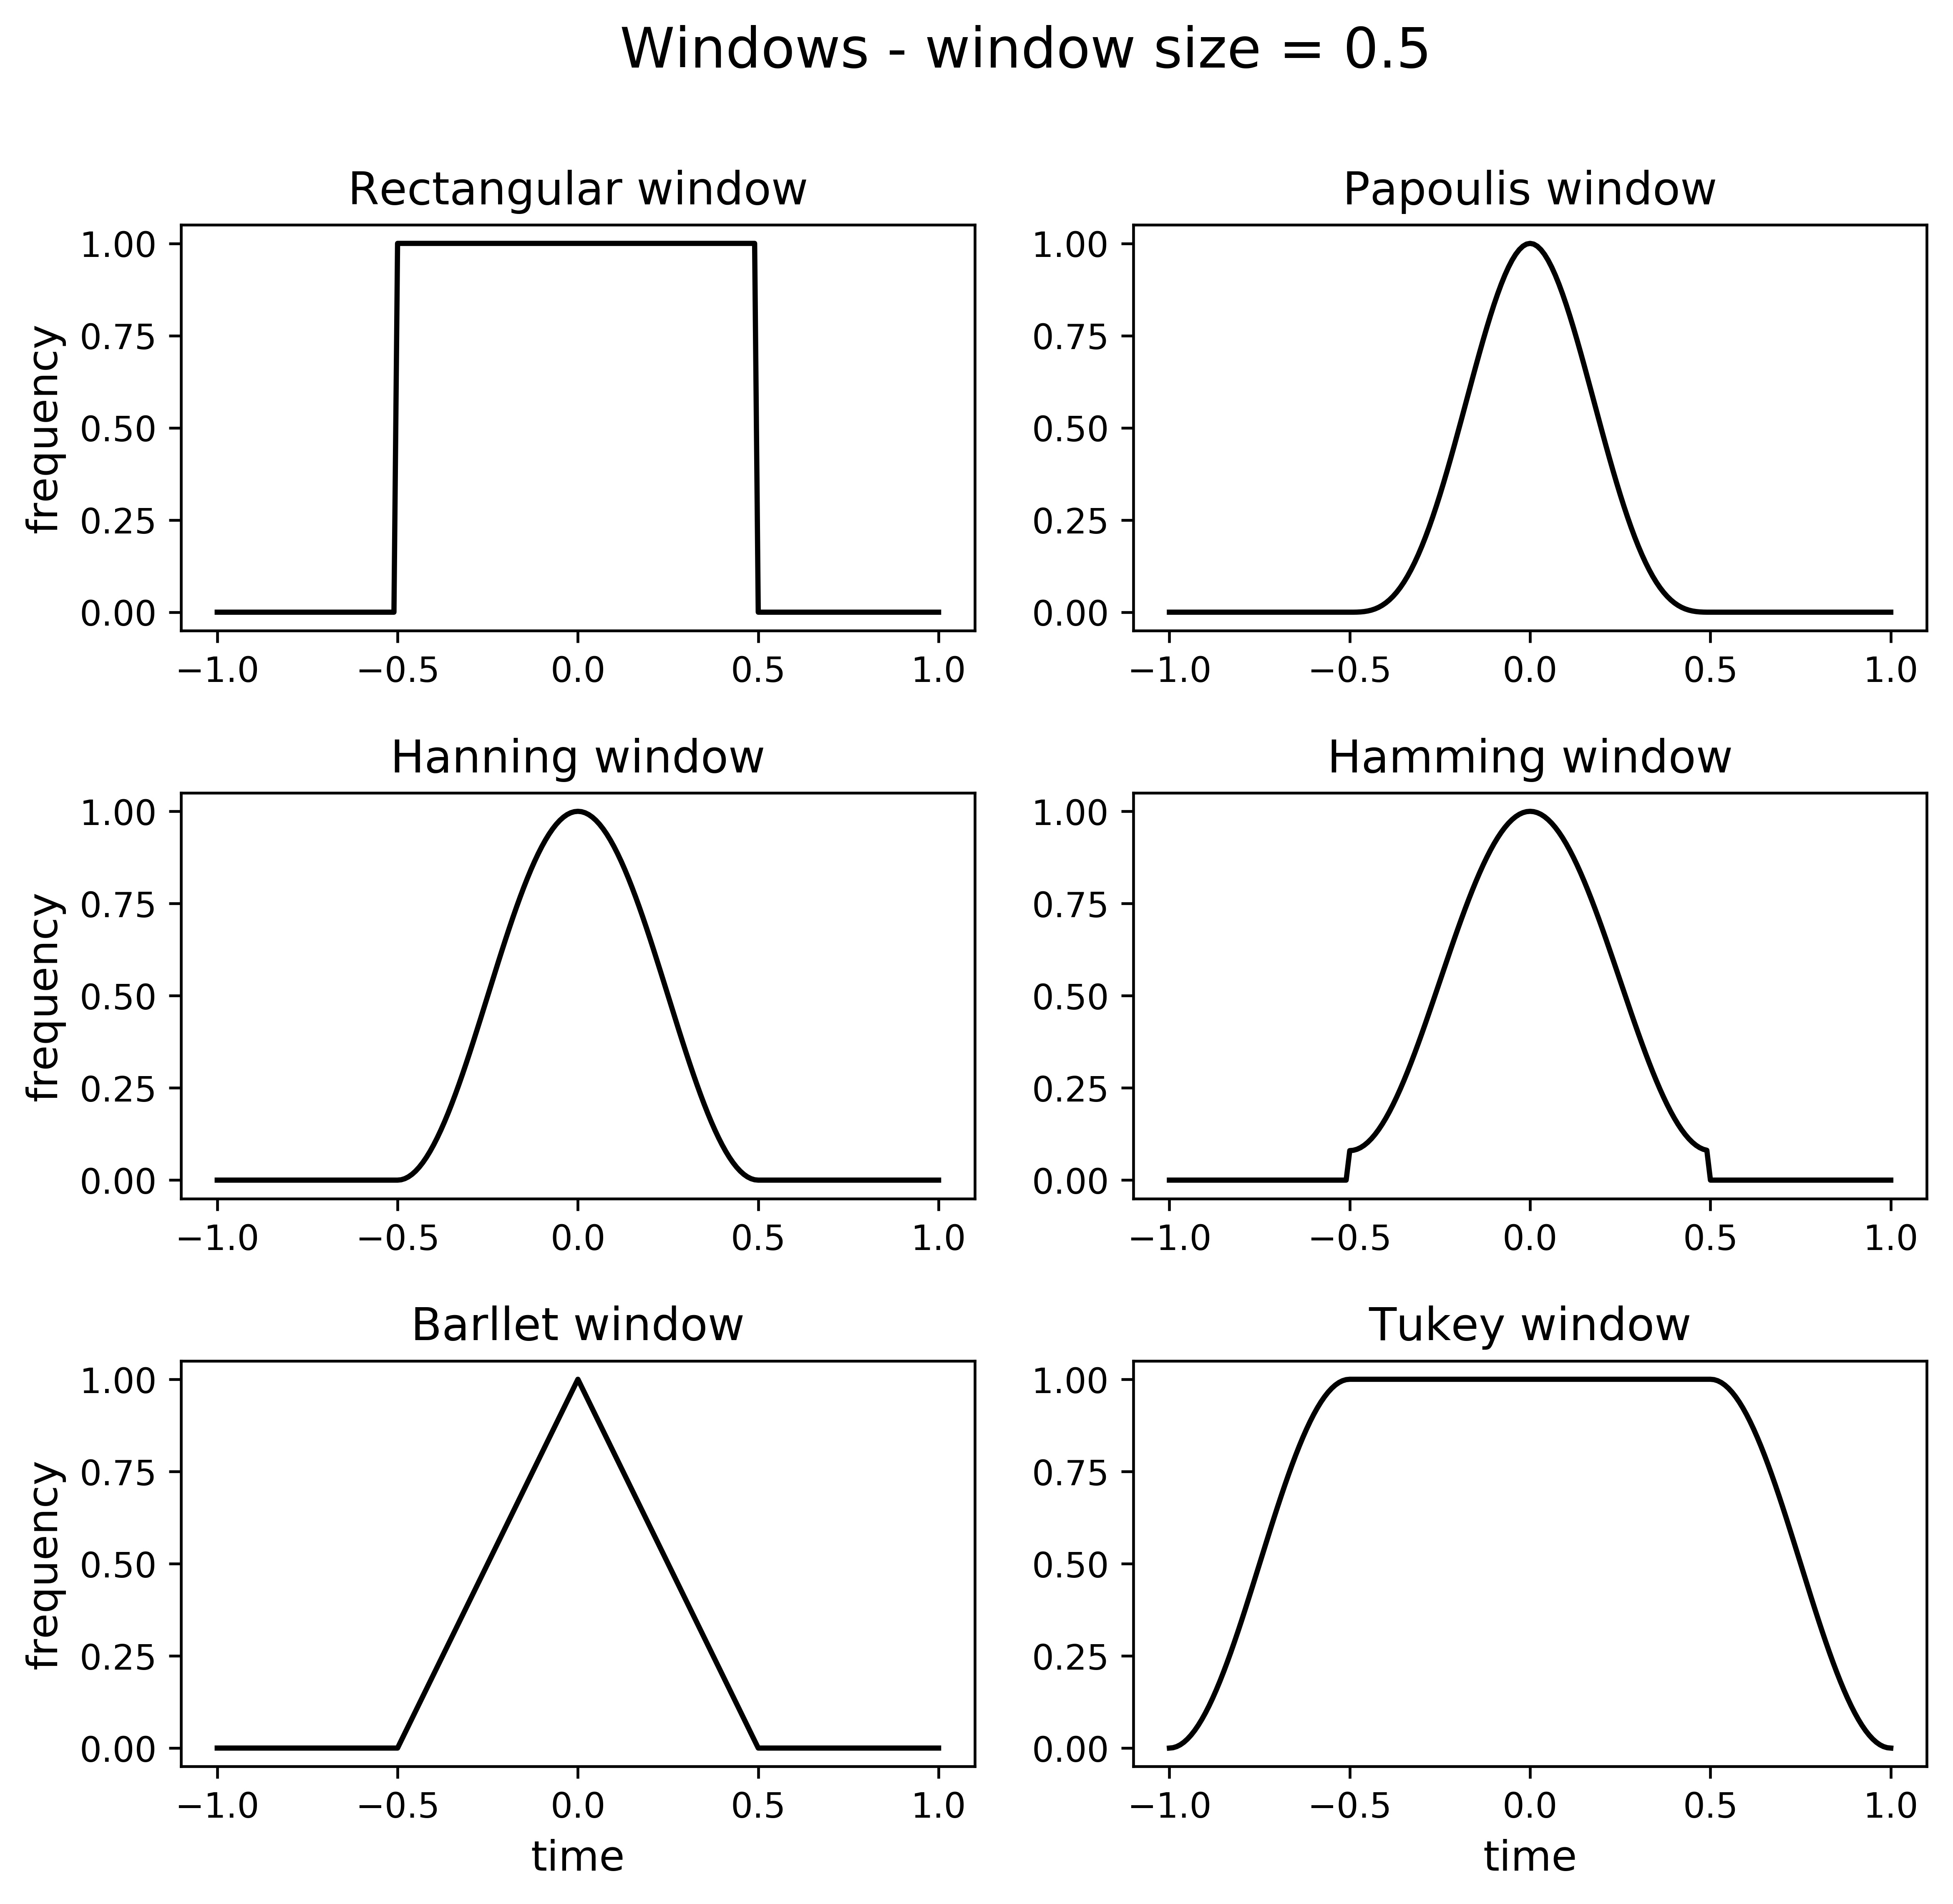
\includegraphics{../scripts/exercicio2/janelas/Windows_plots_ws0.5.jpg}}	
	\end{center}
	\vspace{1mm}	% acrescentar o espaçamento vertical apropriado entre a borda inferior da figura e a legenda ou a fonte quando não há legenda (o valor pode ser negativo para subir)
	%\legenda{Figura 1.1: Dez sinais e seus respectivos histogramas para  asérie com $N$ = 64 do grupo noise.}	% legenda - para deixar sem legenda usar comando \legenda{} (nunca deve-se comentar o comando \legenda)
	\label{ex1_fig1}
	%\FONTE{}	% fonte consultada (elemento obrigatório, mesmo que seja produção do próprio autor)
\end{figure}

% FIGURA
\begin{figure}[ht!]
	\legenda{Figura 2.2: Transformadas de Fourier das funções janela utilizadas neste exercício com largura igual a 0.5.}
	\vspace{2mm}	% acrescentar o espaçamento vertical apropriado entre o título e a borda superior da figura
	\begin{center}
		\resizebox{\textwidth}{!}{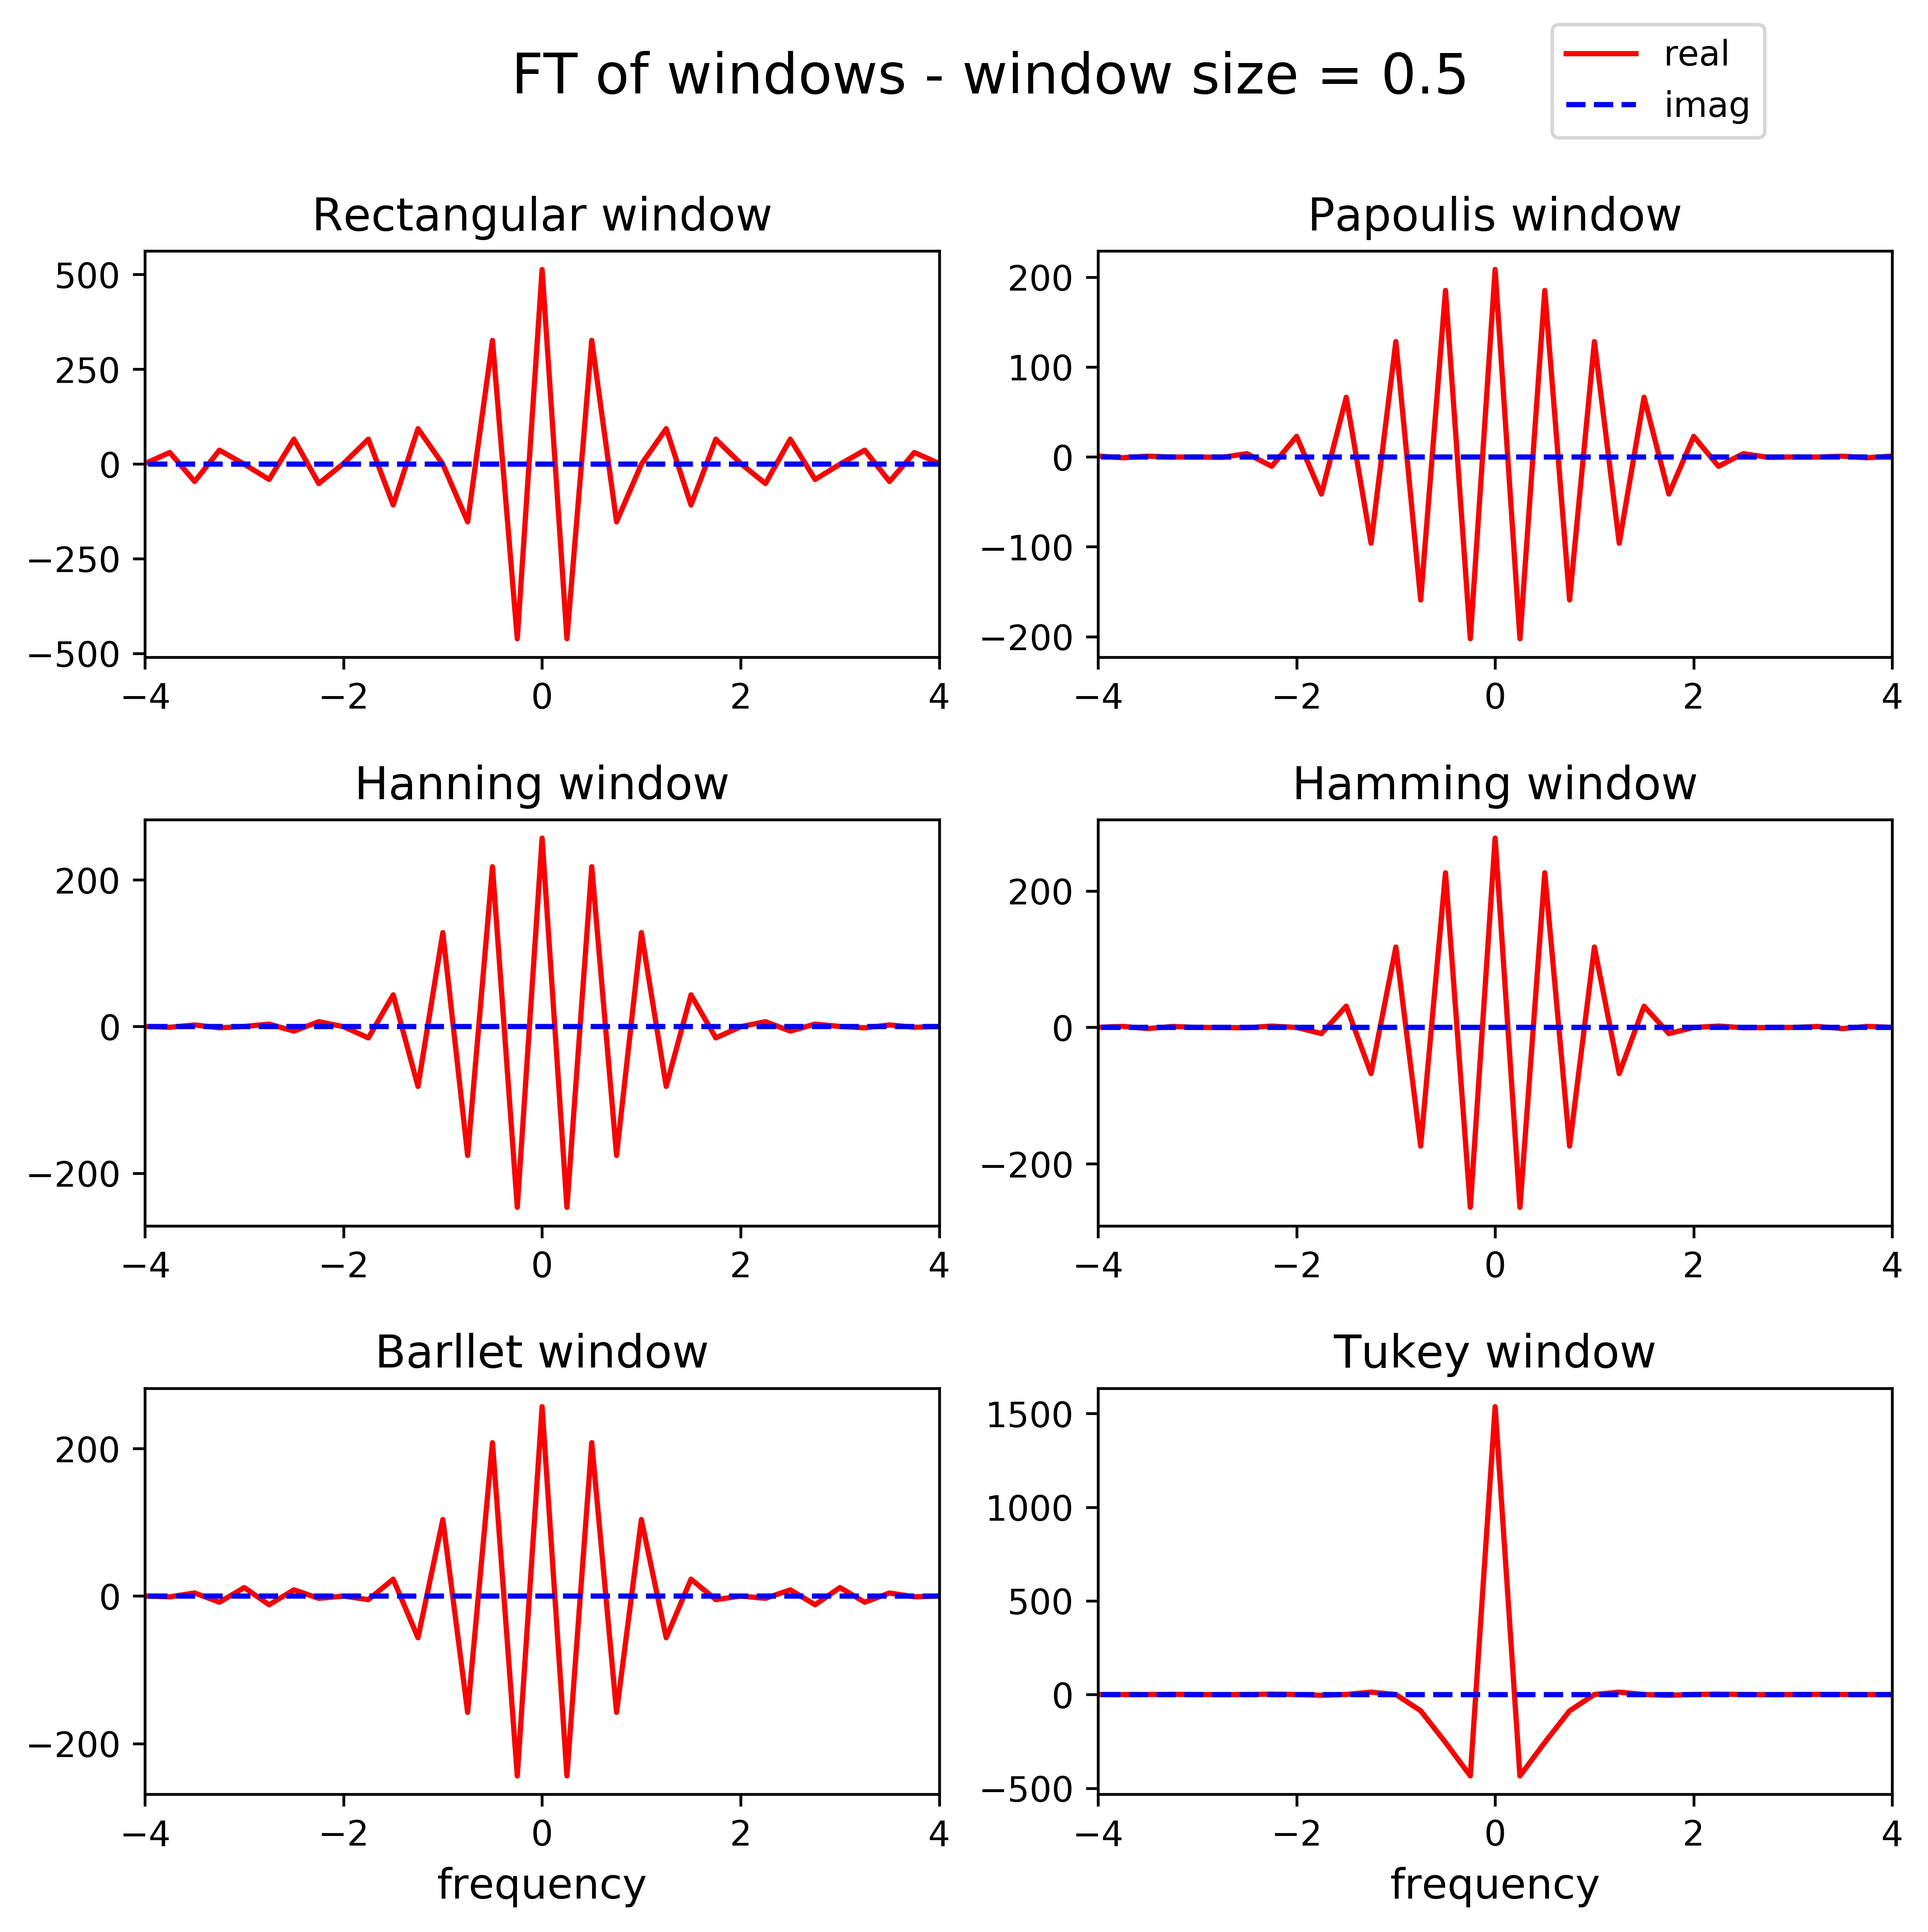
\includegraphics{../scripts/exercicio2/ffts/Windows_FFTs_ws0.5.jpg}}	
	\end{center}
	\vspace{1mm}	% acrescentar o espaçamento vertical apropriado entre a borda inferior da figura e a legenda ou a fonte quando não há legenda (o valor pode ser negativo para subir)
	%\legenda{Figura 1.1: Dez sinais e seus respectivos histogramas para  asérie com $N$ = 64 do grupo noise.}	% legenda - para deixar sem legenda usar comando \legenda{} (nunca deve-se comentar o comando \legenda)
	\label{ex1_fig1}
	%\FONTE{}	% fonte consultada (elemento obrigatório, mesmo que seja produção do próprio autor)
\end{figure}


As mesmas janelas, porém com tamanho igual a 0.1, produzem os resultados das Figuras 2.3 e 2.4. 


% FIGURA
\begin{figure}[ht!]
	\legenda{Figura 2.3: Gráfico das seis janelas utilizadas neste exercício com largura (abaixo denominado \texttt{window size}) igual a 0.1.}
	\vspace{2mm}	% acrescentar o espaçamento vertical apropriado entre o título e a borda superior da figura
	\begin{center}
		\resizebox{\textwidth}{!}{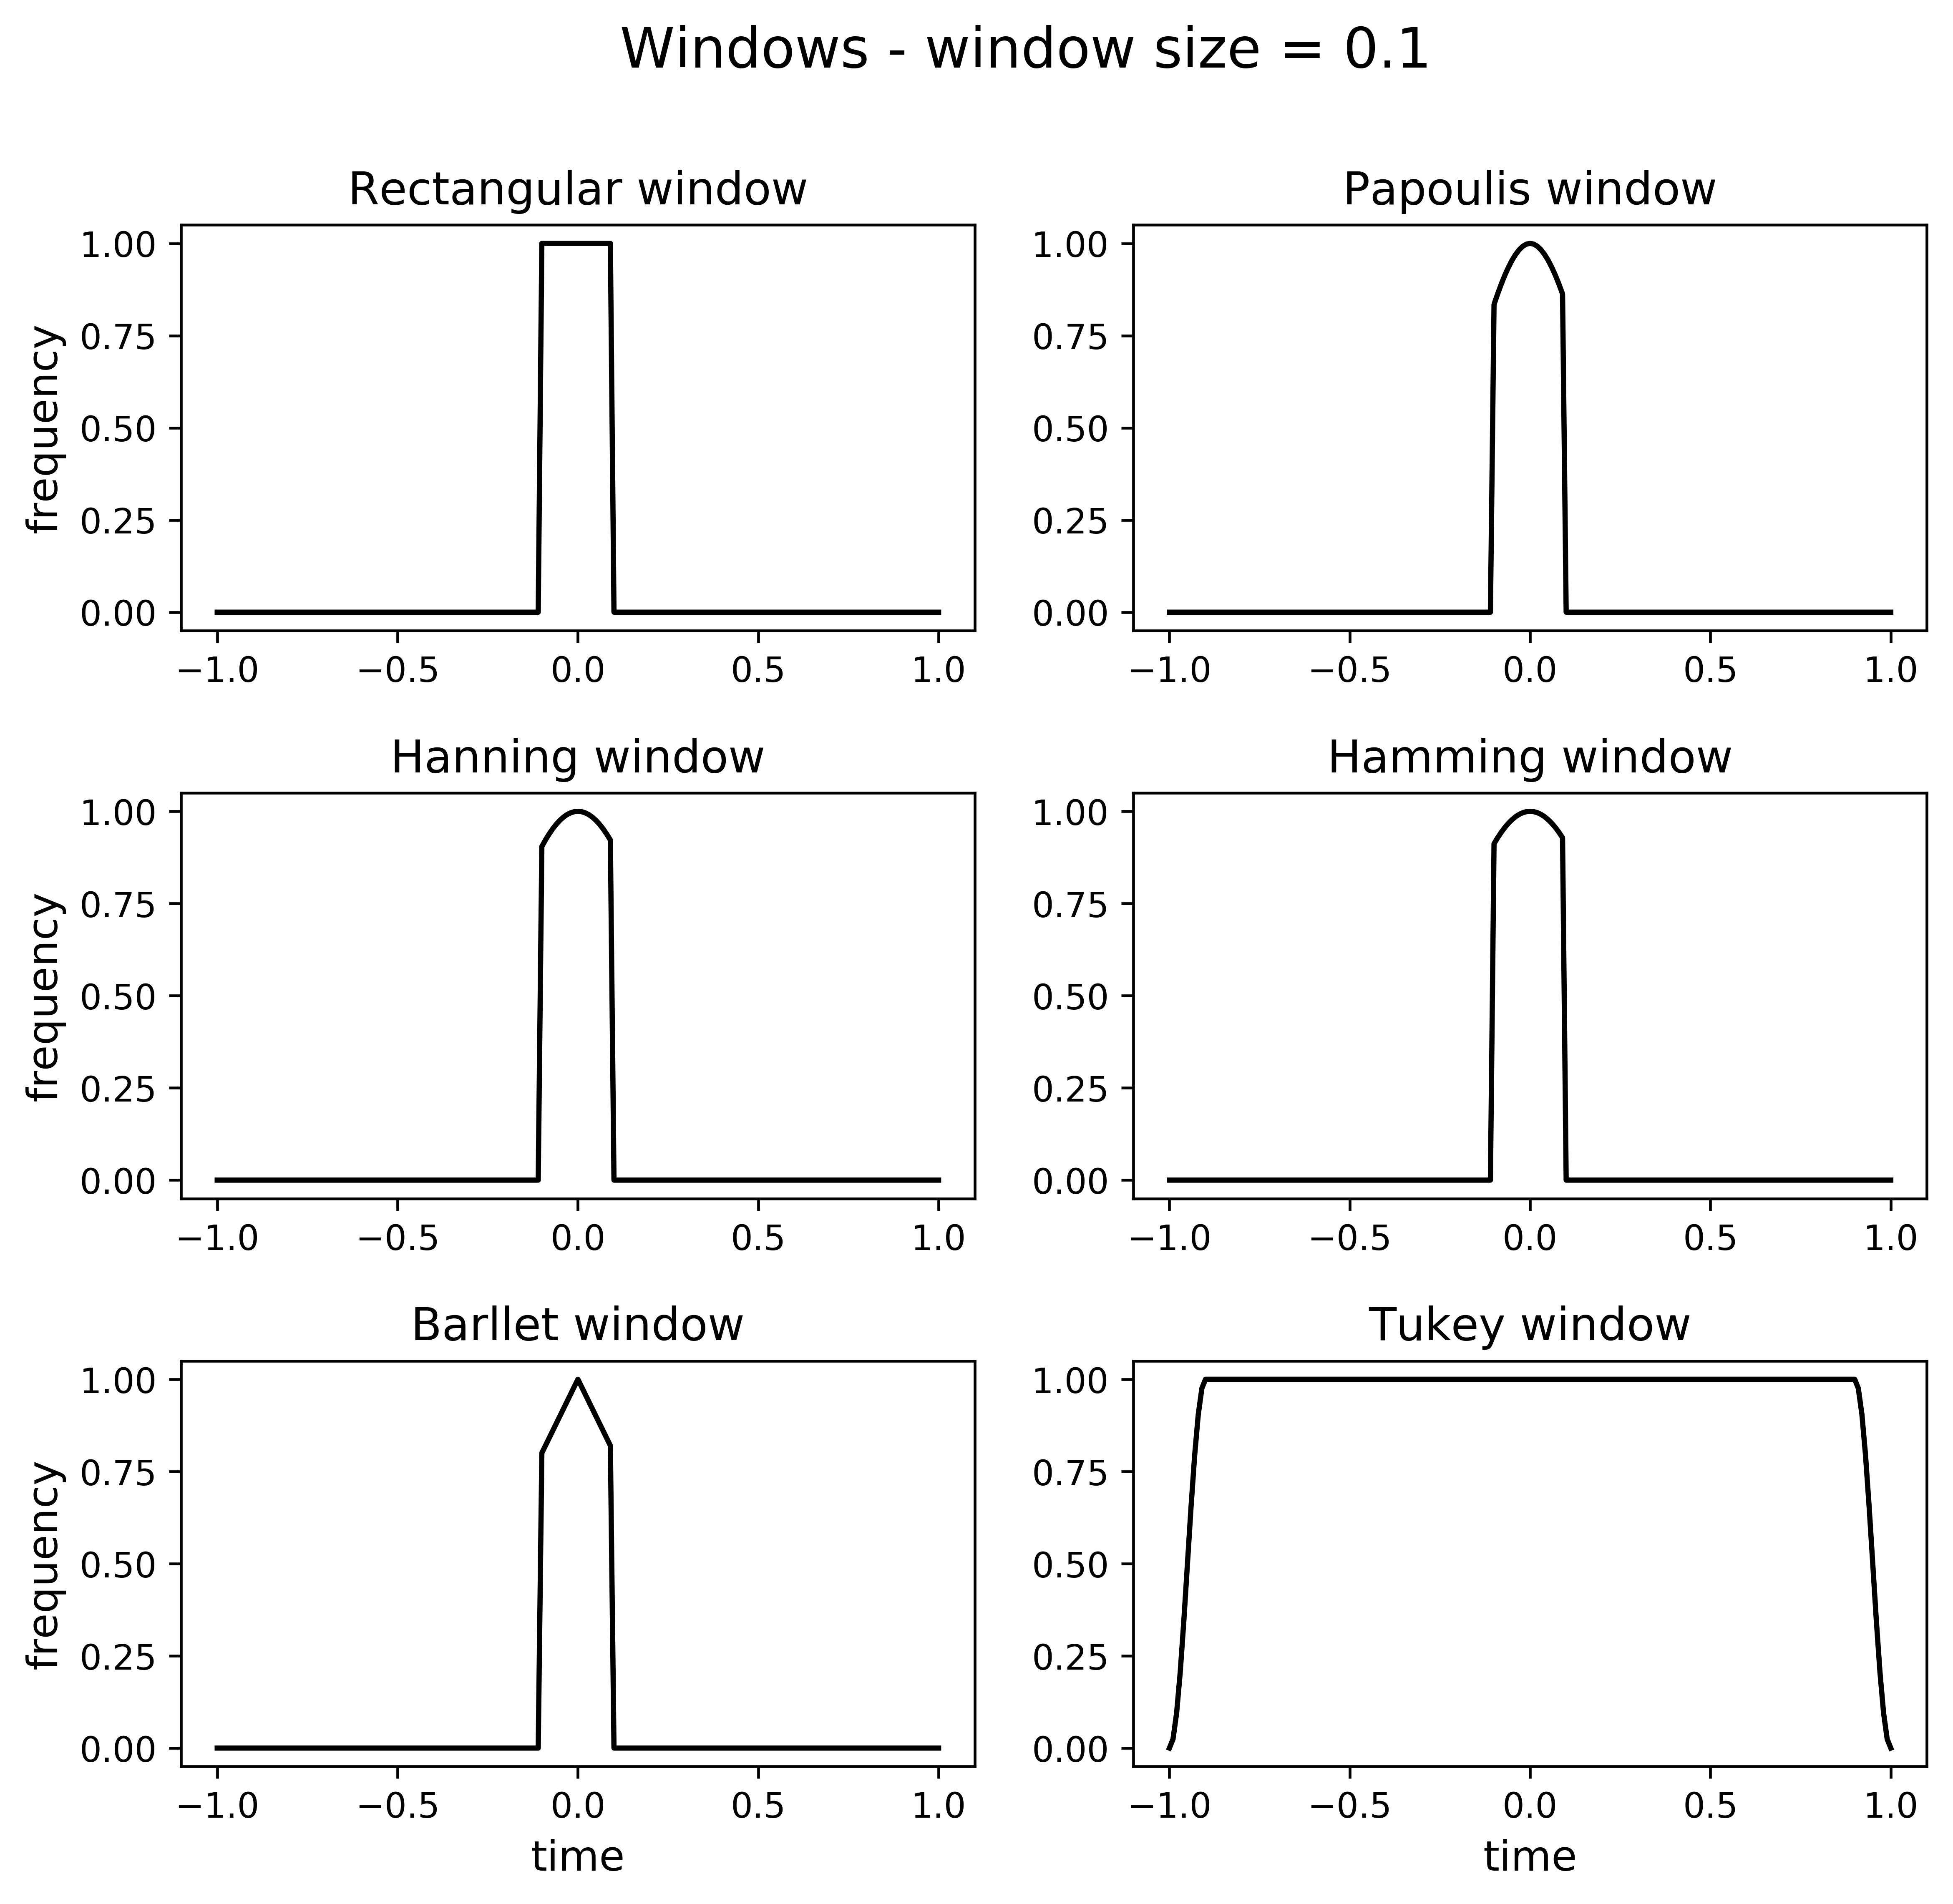
\includegraphics{../scripts/exercicio2/janelas/Windows_plots_ws0.1.jpg}}	
	\end{center}
	\vspace{1mm}	% acrescentar o espaçamento vertical apropriado entre a borda inferior da figura e a legenda ou a fonte quando não há legenda (o valor pode ser negativo para subir)
	%\legenda{Figura 1.1: Dez sinais e seus respectivos histogramas para  asérie com $N$ = 64 do grupo noise.}	% legenda - para deixar sem legenda usar comando \legenda{} (nunca deve-se comentar o comando \legenda)
	\label{ex1_fig1}
	%\FONTE{}	% fonte consultada (elemento obrigatório, mesmo que seja produção do próprio autor)
\end{figure}

% FIGURA
\begin{figure}[ht!]
	\legenda{Figura 2.4: Transformadas de Fourier das funções janela utilizadas neste exercício com largura igual a 0.1.}
	\vspace{2mm}	% acrescentar o espaçamento vertical apropriado entre o título e a borda superior da figura
	\begin{center}
		\resizebox{\textwidth}{!}{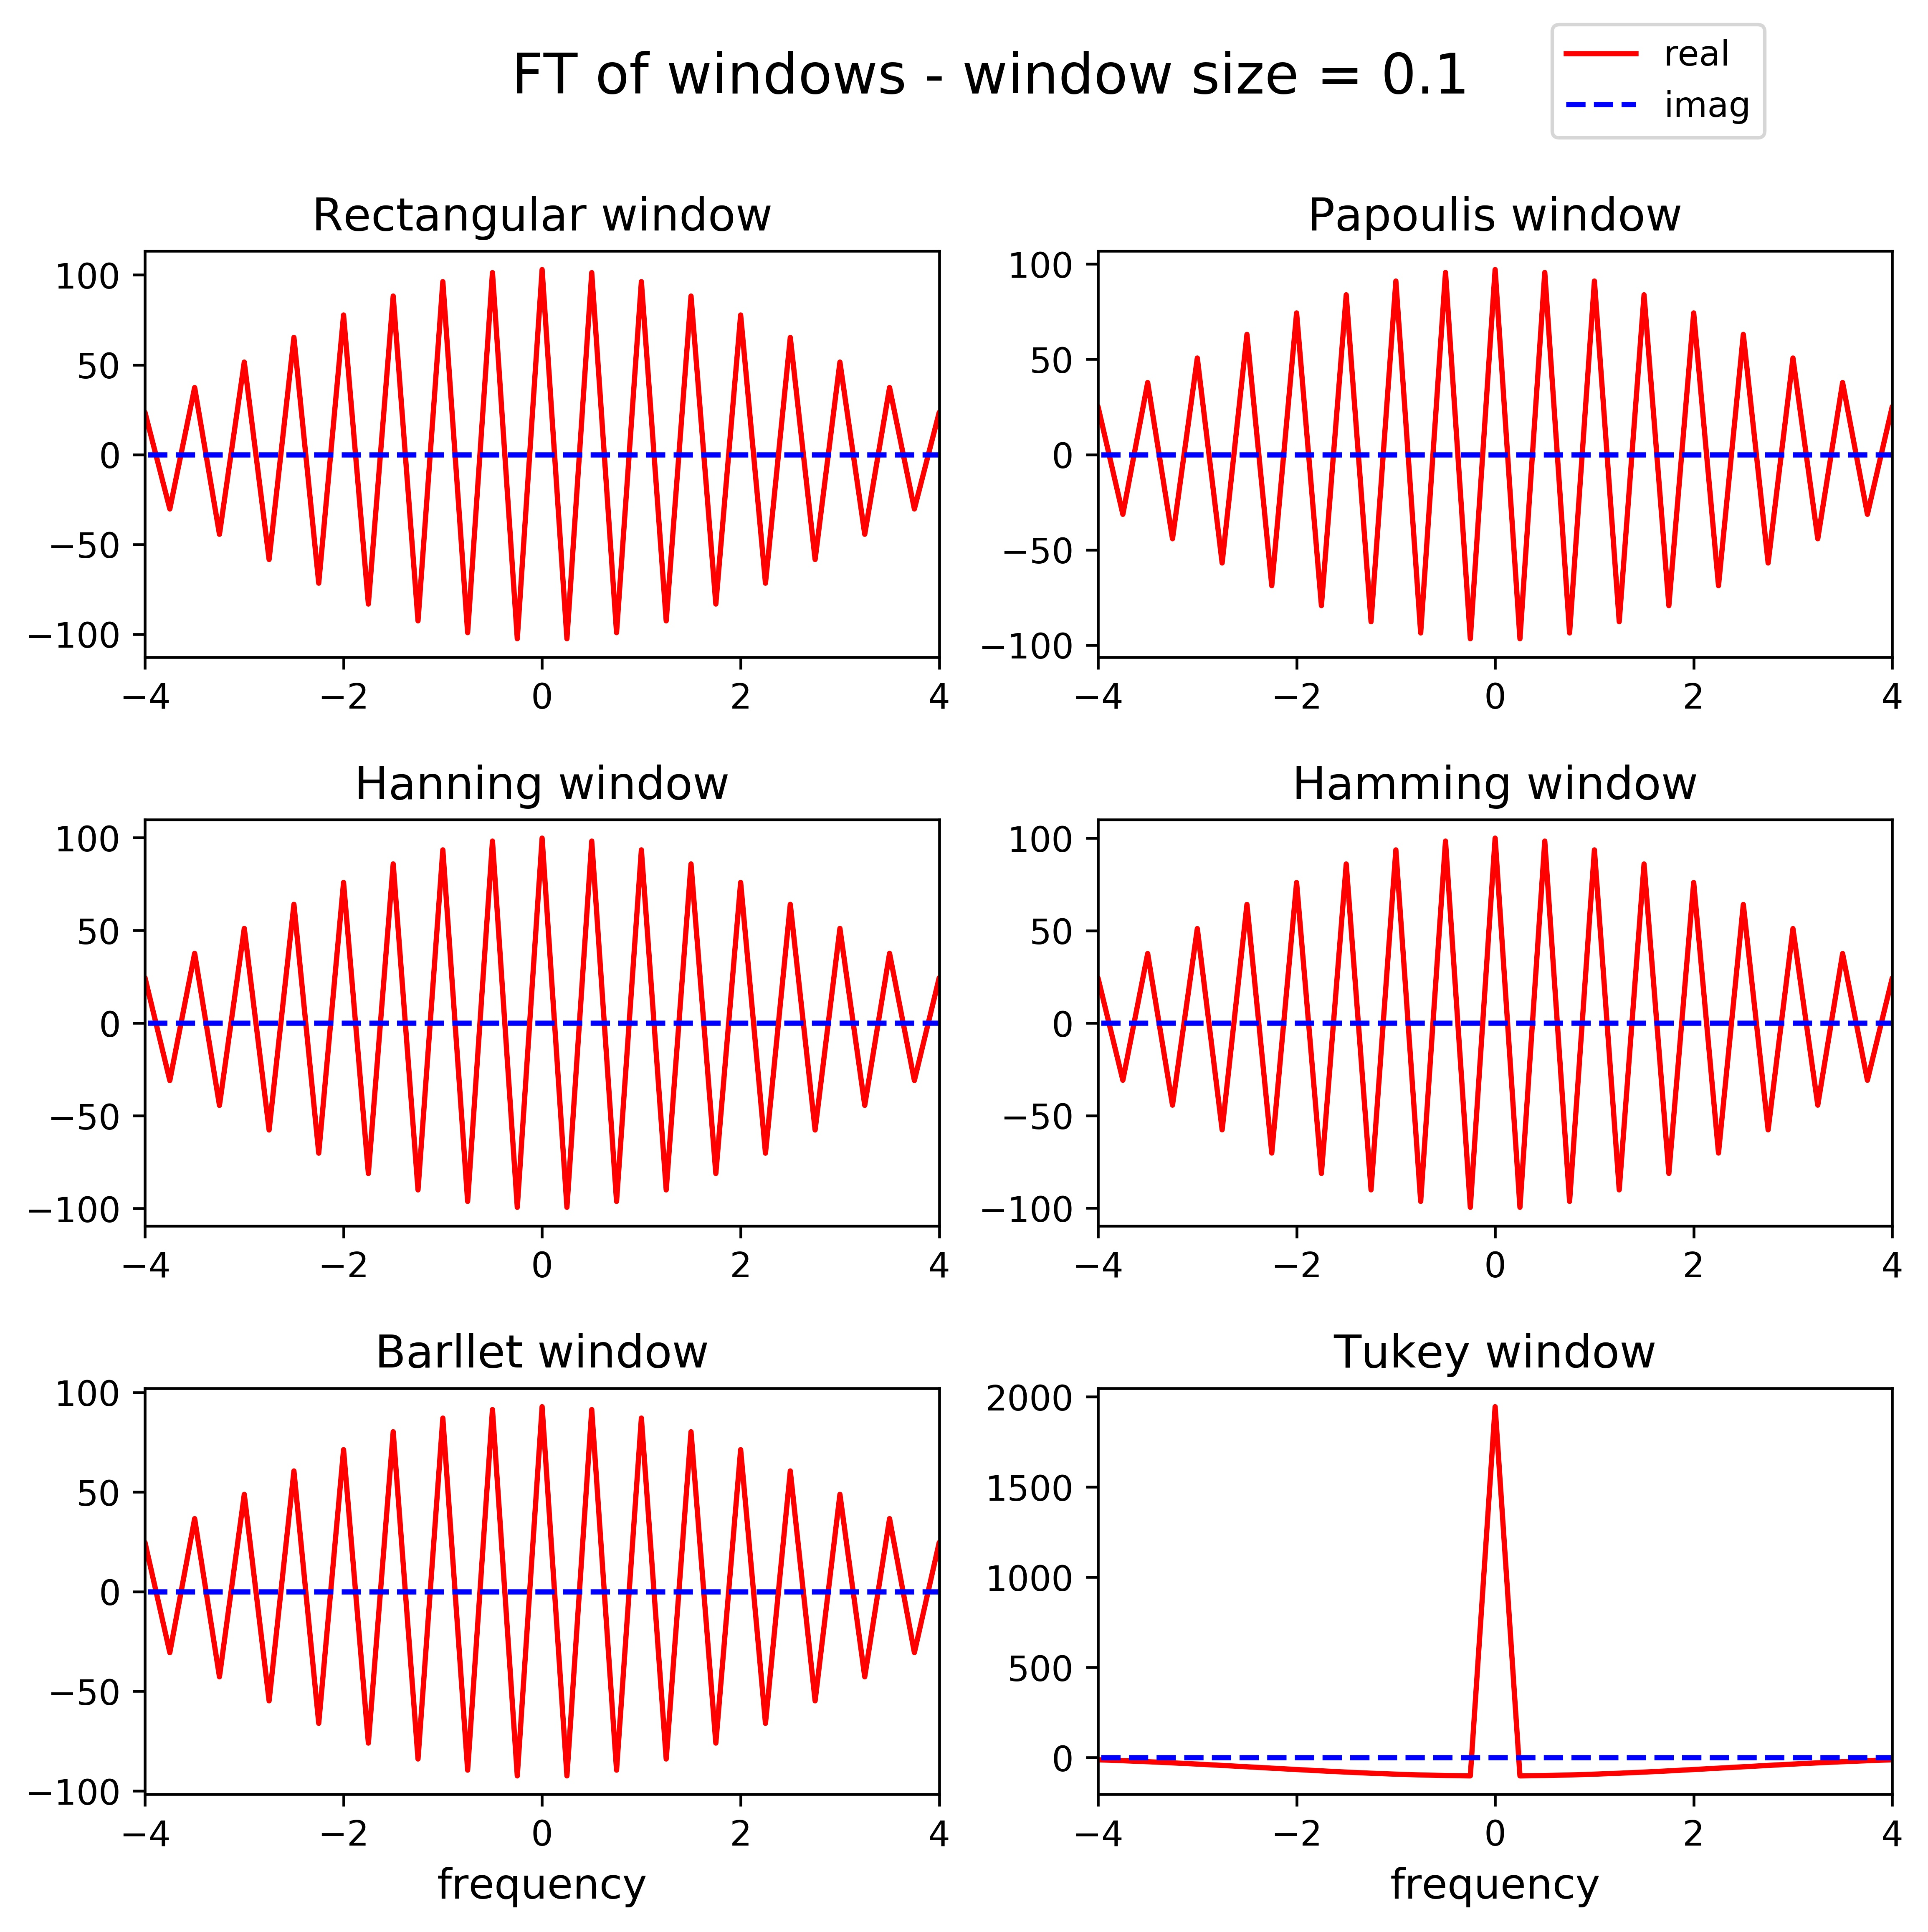
\includegraphics{../scripts/exercicio2/ffts/Windows_FFTs_ws0.1.jpg}}	
	\end{center}
	\vspace{1mm}	% acrescentar o espaçamento vertical apropriado entre a borda inferior da figura e a legenda ou a fonte quando não há legenda (o valor pode ser negativo para subir)
	%\legenda{Figura 1.1: Dez sinais e seus respectivos histogramas para  asérie com $N$ = 64 do grupo noise.}	% legenda - para deixar sem legenda usar comando \legenda{} (nunca deve-se comentar o comando \legenda)
	\label{ex1_fig1}
	%\FONTE{}	% fonte consultada (elemento obrigatório, mesmo que seja produção do próprio autor)
\end{figure}


%%%%%%%%%%%%%%%%%%%%%%%%%%%%%%%%%%%%%%%%%%%%%%%%%%%%%%%%%% 2.b

\clearpage
\subsection*{2.b} 
\addcontentsline{toc}{section}{\protect\numberline{} 2.b}%

Dada uma escolha do sinal (variável \texttt{chirp} abaixo, à qual é atribuída um dos chirps do Exercício 1), os espectrogramas foram calculados a partir do método \texttt{spec}, recebendo como input: o produto do chirp e da função janela \textit{shiftada}, a resolução \texttt{res} (para cálculo dos bins de frequência), a frequência final de interesse \texttt{f\_final}, e o número de bins \texttt{N} com o qual a FFT será implementada.

\lstinputlisting[language=python, style=mystyle, firstline=298, lastline=348]{../scripts/exercicio2/espectros/window_spectra.py}

A seguir são apresentados os resultados das WFT de cada chirp do Exercício 1. Dois valores foram usados para o tamanho das janelas implementadas e dois domínios diferentes para cada chirp (a saber, os domínios referentes às Figuras 1.1 e 1.2). O espectrograma de cada caso foi gerado.

As figuras dos espectrogramas foram criadas com o pacote \texttt{matplotlib}, em particular com a função \texttt{countourf}. Foi utilizando o mapa de cor \texttt{jet} e 256 níveis de cor. Cada figura possui o mesmo intervalo de cor em sua representação (mesmos \texttt{vmin} e \texttt{vmax}). O trecho do código que gera a visualização das Figuras 2.4 a 2.16 é exibido abaixo:
\lstinputlisting[language=python, style=mystyle, firstline=352, lastline=411]{../scripts/exercicio2/espectros/window_spectra.py}

%%%%%%%%%%%%%%%% Gaussiano


Espectrogramas do \textbf{chirp gaussiano}, $-2 \leq t \leq 2$ e tamanho das janelas = 0.1: Figura 2.4.

% FIGURA
\begin{figure}[ht!]
	\legenda{Figura 2.4: Espectrogramas do chirp gaussiano com as seis funções janela usadas neste exercício de tamanho (largura) igual a 0.1. Comparar com o topo da Figura 1.1.}
	\vspace{3mm}	
	\begin{center}
		\resizebox{\textwidth}{!}{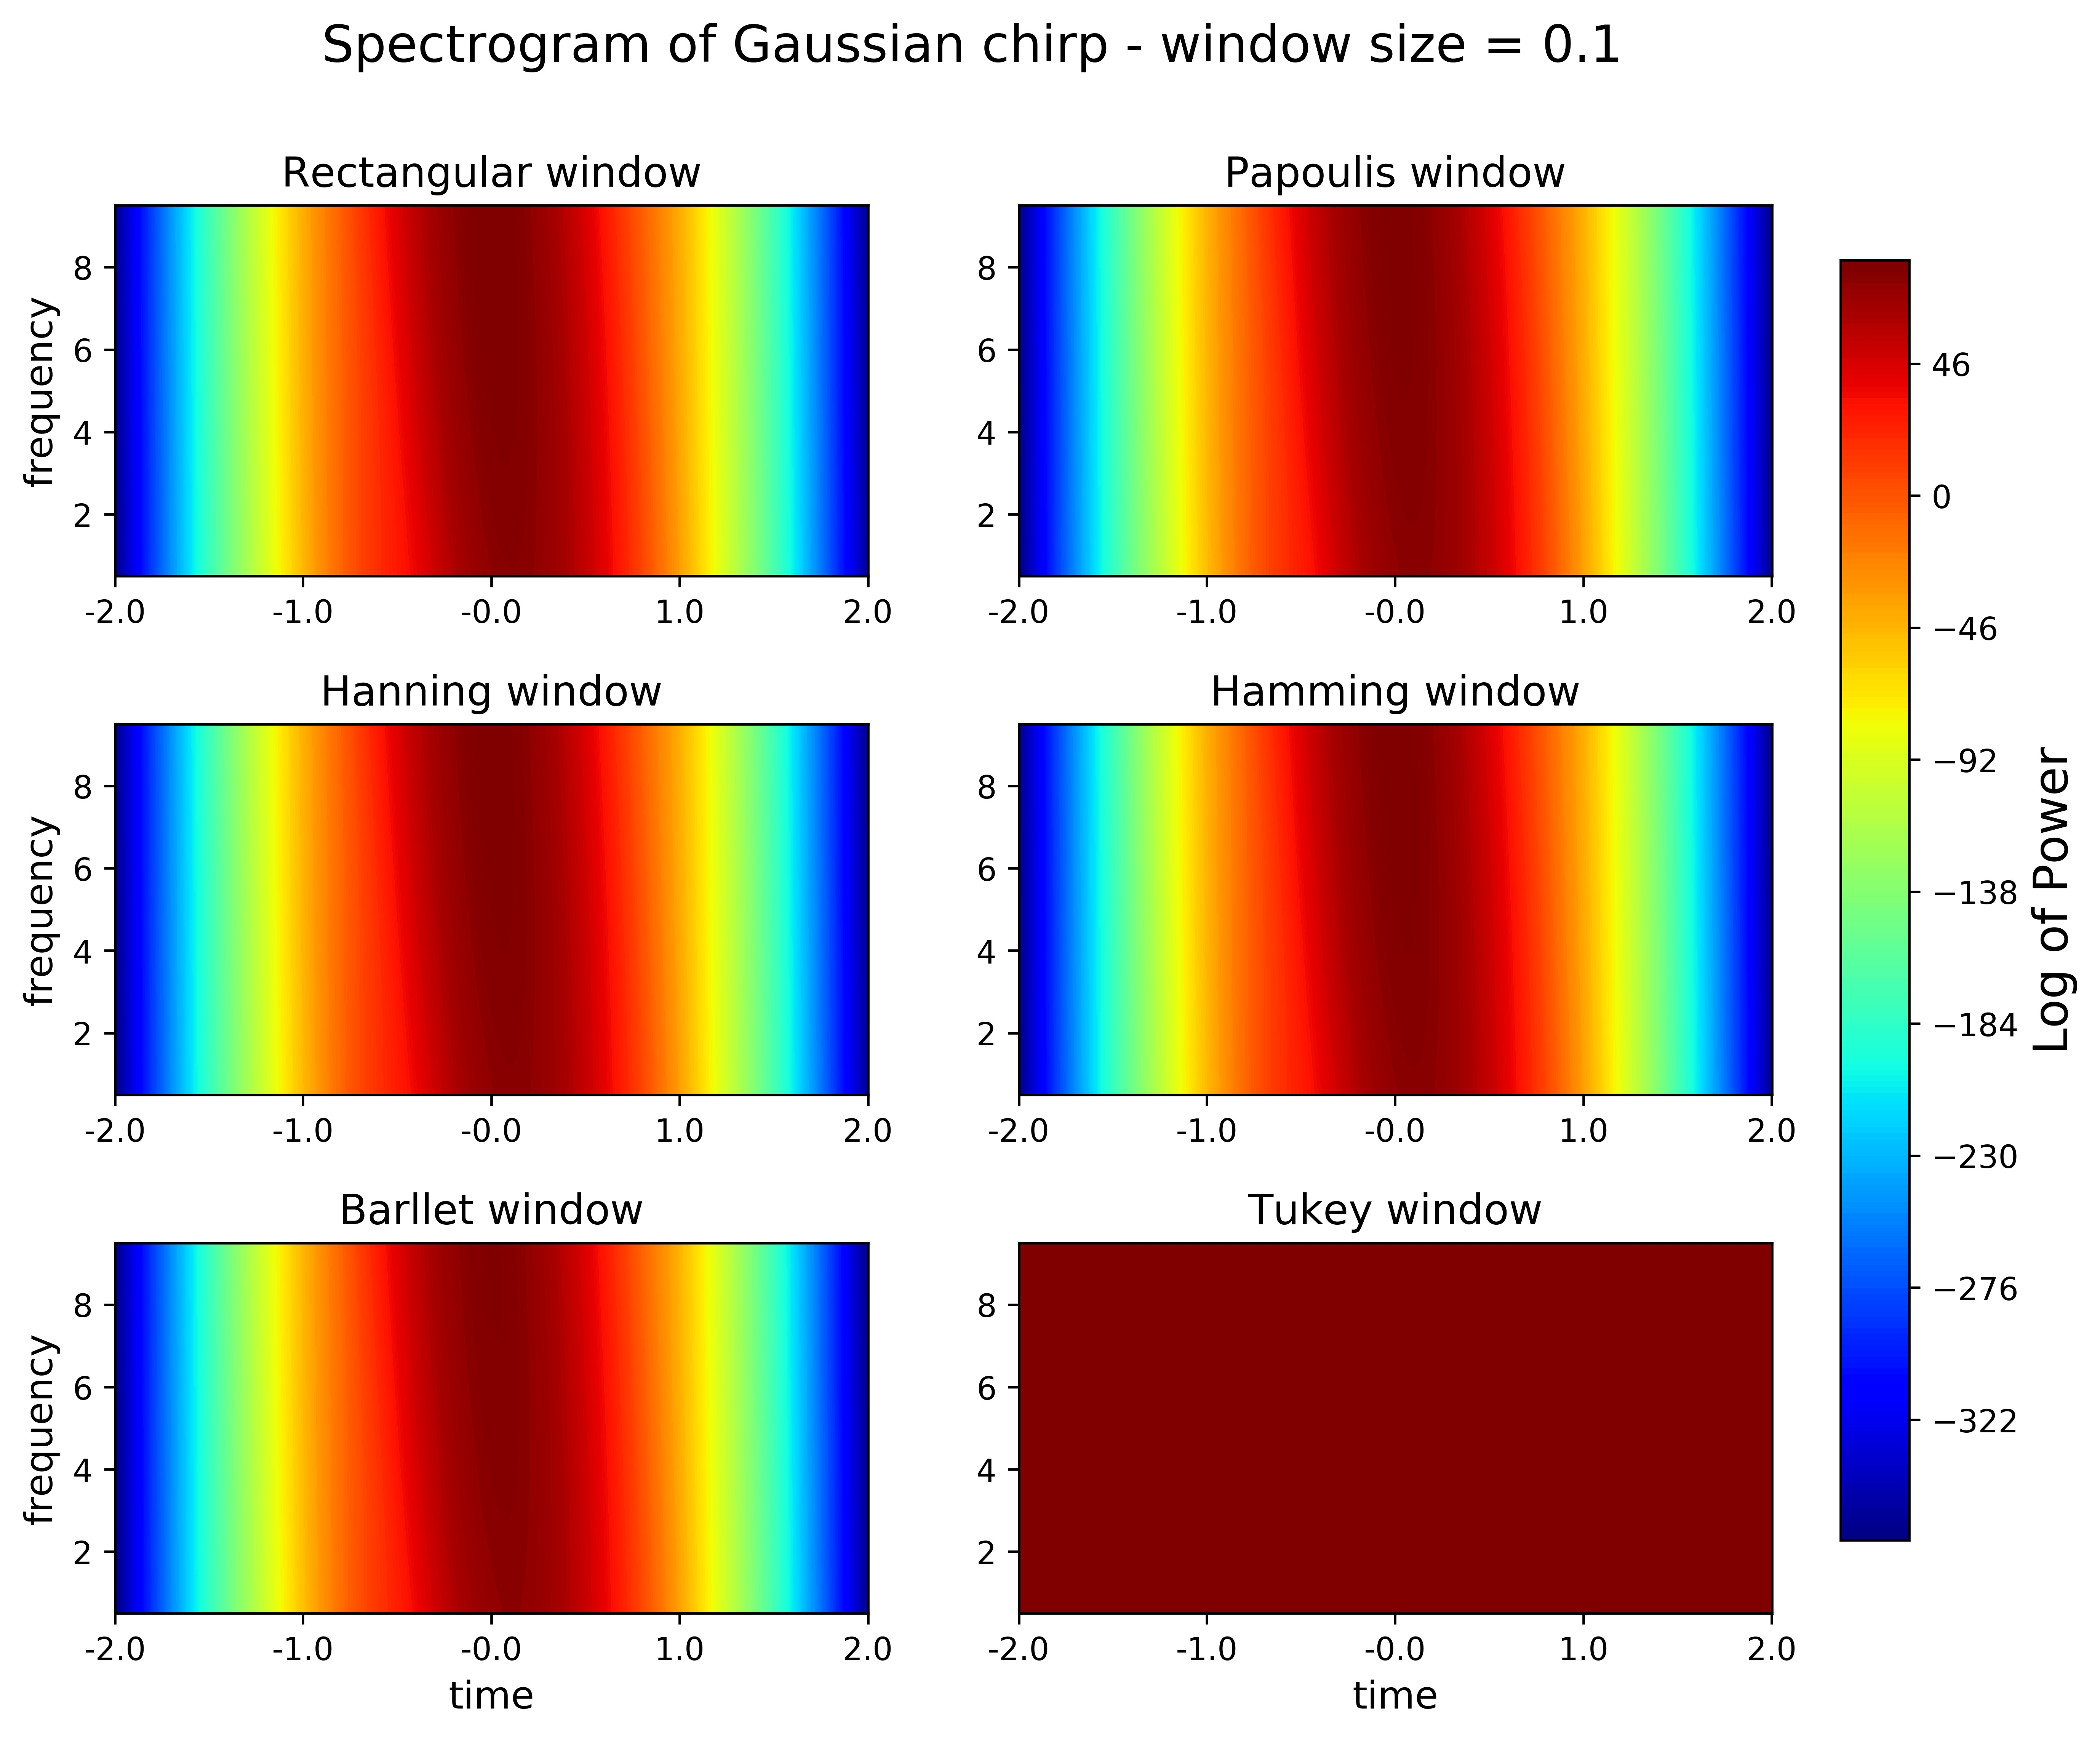
\includegraphics{../scripts/exercicio2/espectros/Gaussian_ws0.1.jpg}}	
	\end{center}
	\vspace{1mm}	
	\label{ex1_fig1}
\end{figure}

Espectrogramas do \textbf{chirp gaussiano}, $-2 \leq t \leq 2$ e tamanho das janelas = 0.5: Figura 2.5.

% FIGURA
\begin{figure}[ht!]
	\legenda{Figura 2.5: Espectrogramas do chirp gaussiano com as seis funções janela usadas neste exercício de tamanho (largura) igual a 0.5. Comparar com o topo da Figura 1.1.}
	\vspace{3mm}	
	\begin{center}
		\resizebox{\textwidth}{!}{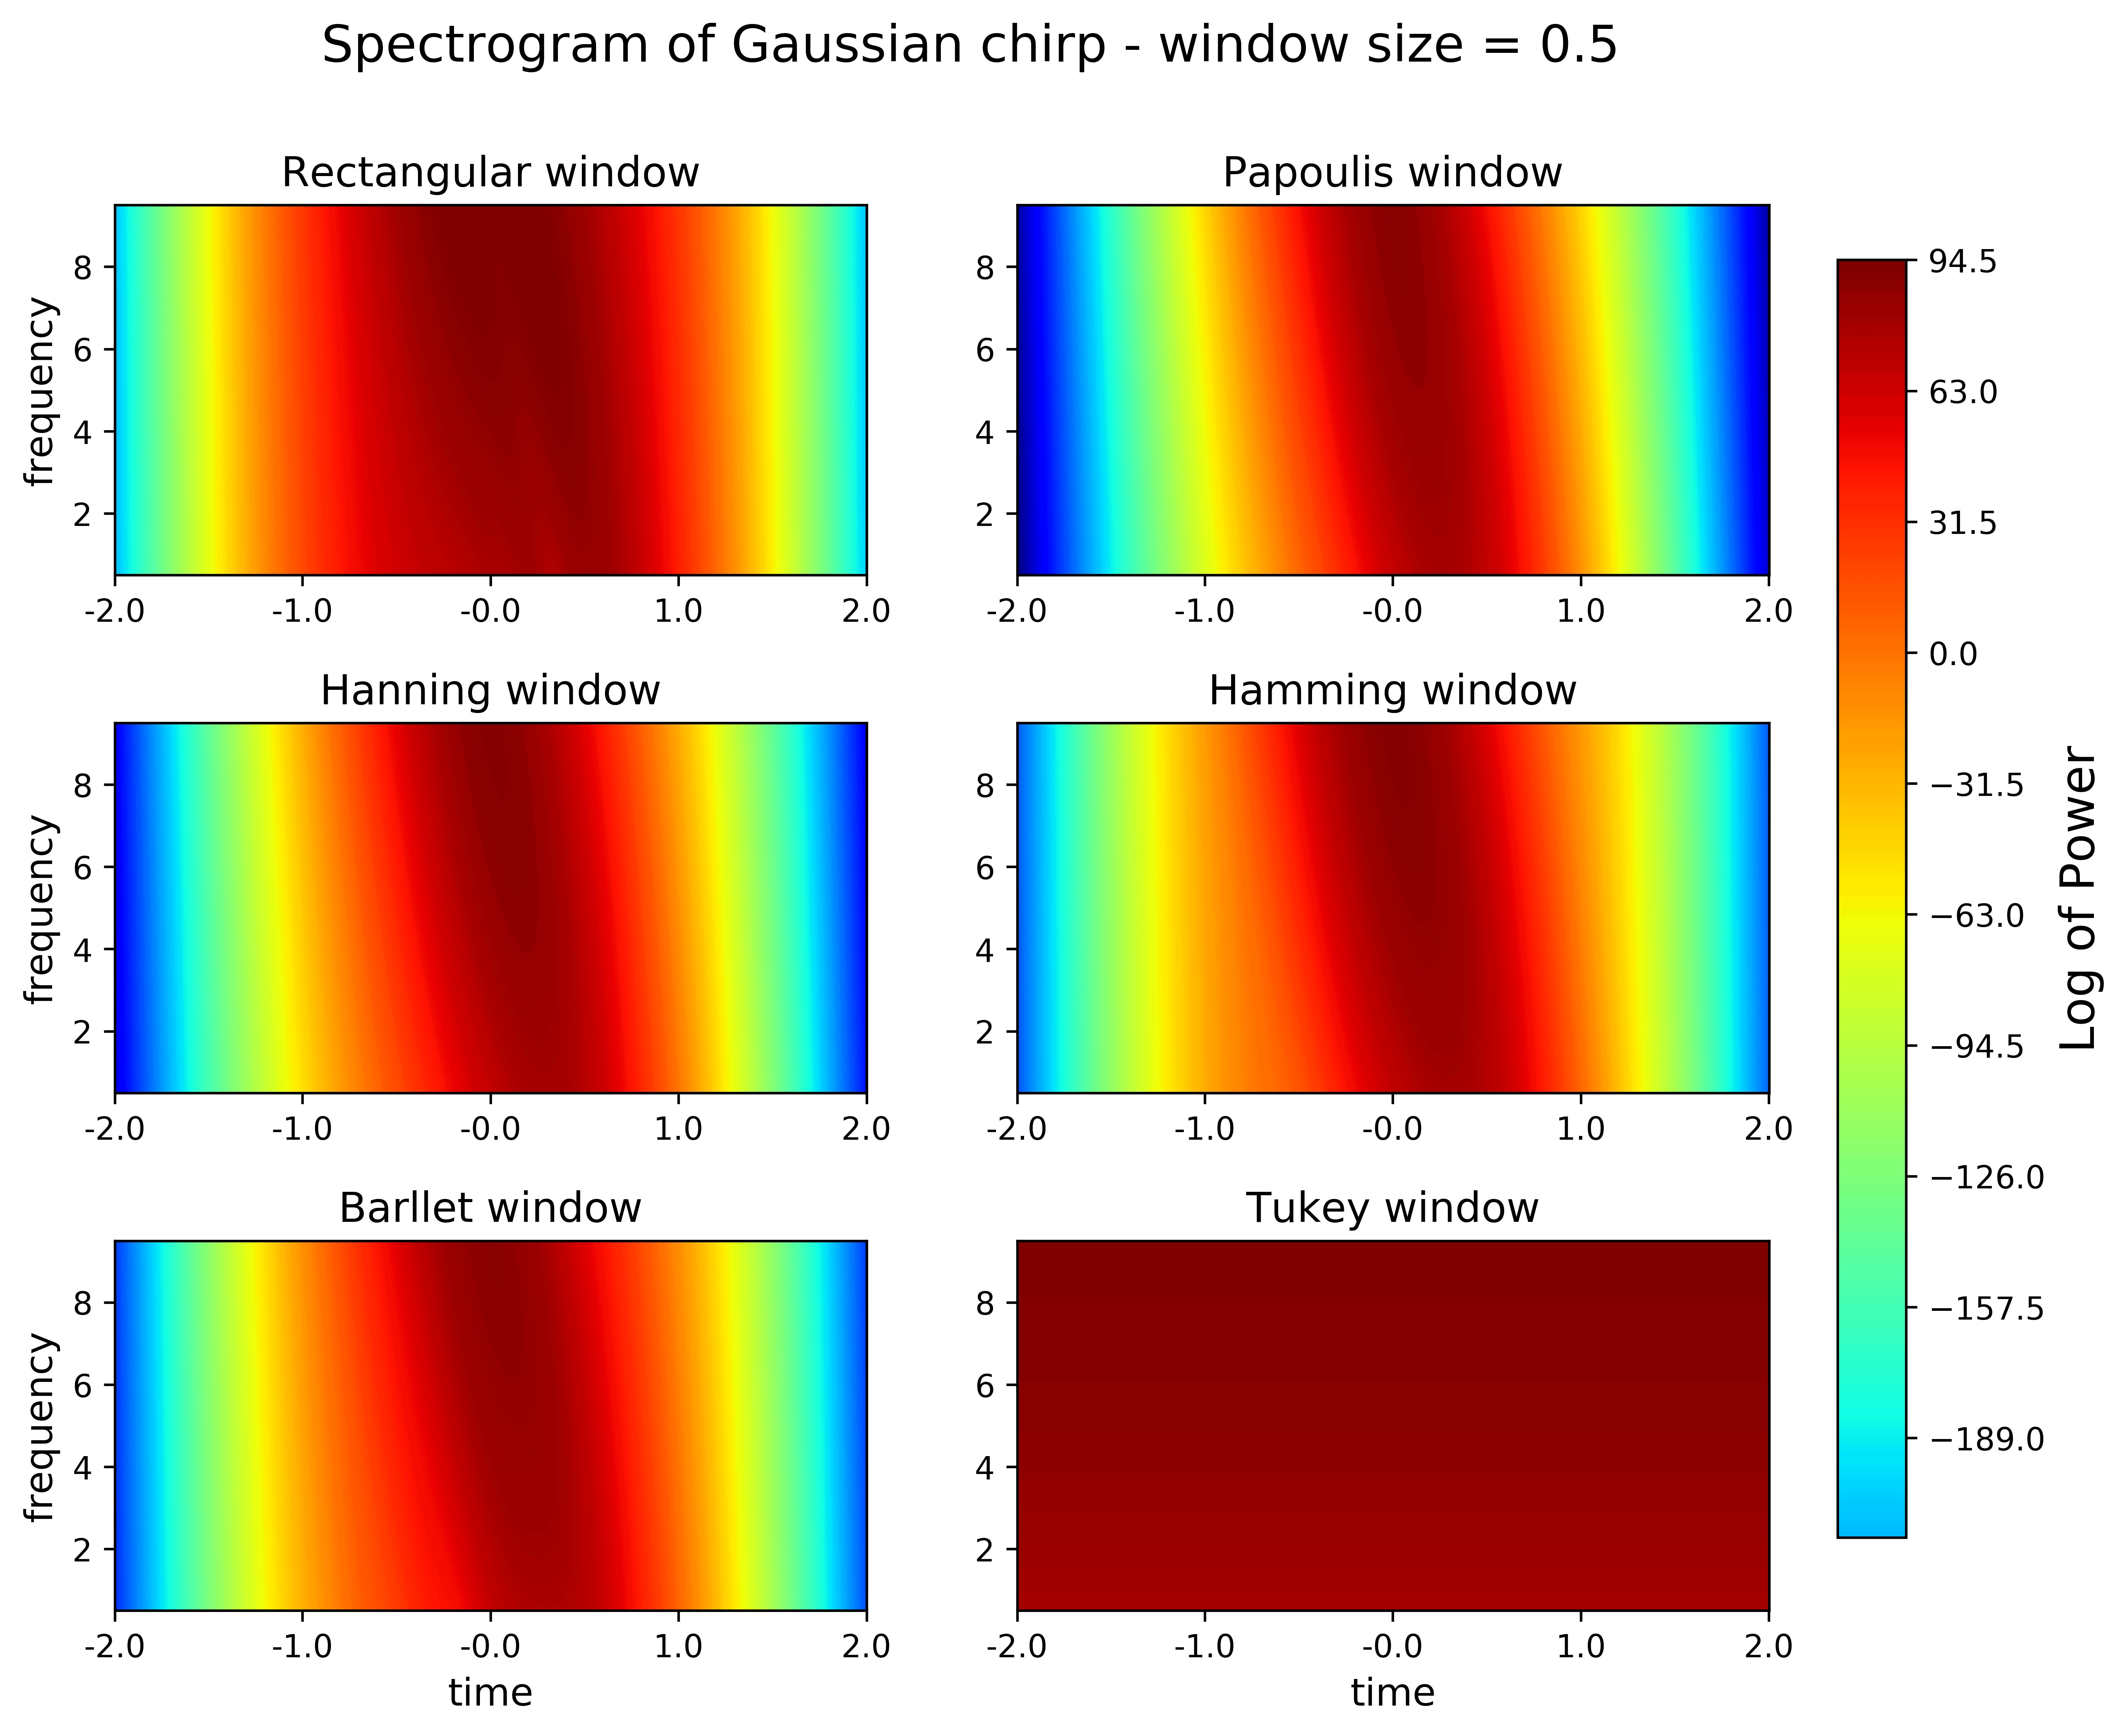
\includegraphics{../scripts/exercicio2/espectros/Gaussian_ws0.5.jpg}}	
	\end{center}
	\vspace{1mm}
	\label{ex1_fig1}
\end{figure}


Espectrogramas do \textbf{chirp gaussiano}, $0 \leq t \leq 6$ e tamanho das janelas = 0.5: Figura 2.6.

% FIGURA
\begin{figure}[ht!]
	\legenda{Figura 2.6: Espectrogramas do chirp gaussiano com as seis funções janela usadas neste exercício de tamanho (largura) igual a 0.5. Comparar com o topo da Figura 1.3.}
	\vspace{3mm}	
	\begin{center}
		\resizebox{\textwidth}{!}{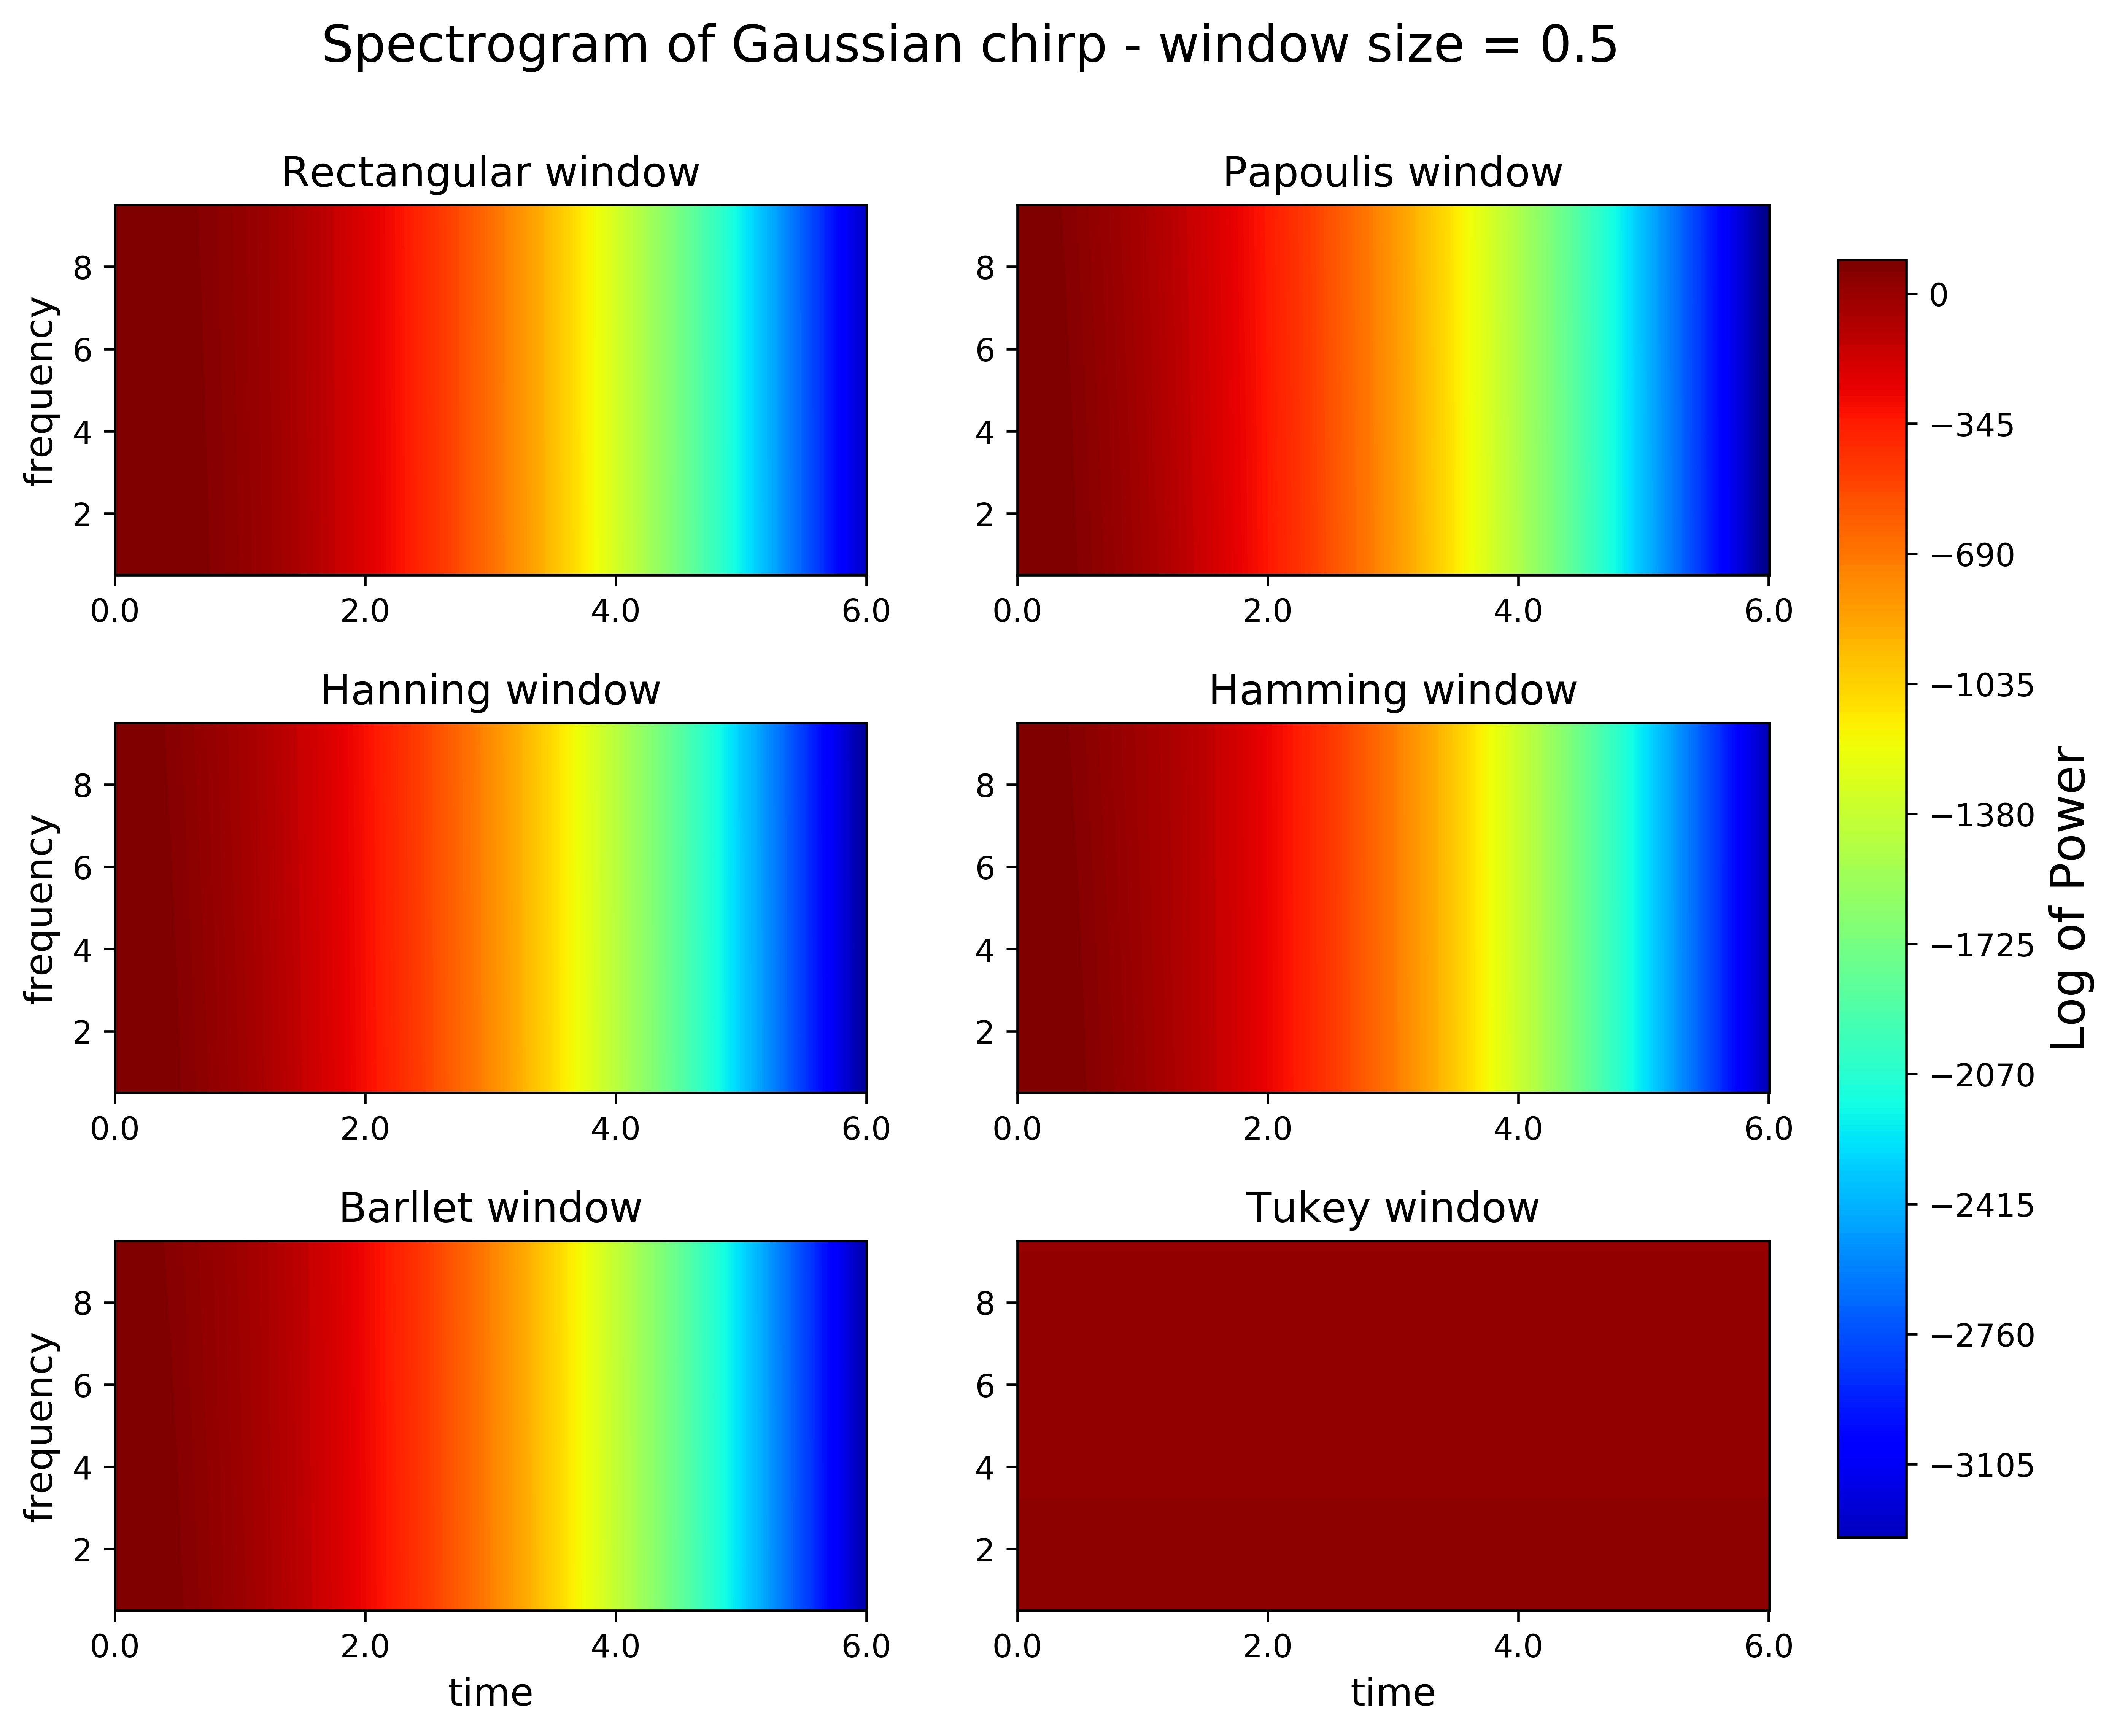
\includegraphics{../scripts/exercicio2/espectros/TEST_Gaussian_ws0.5.jpg}}	
	\end{center}
	\vspace{1mm}
	\label{ex1_fig1}
\end{figure}


%%%%%%%%%%%%%%%% Linear


Espectrogramas do \textbf{chirp linear}, $-6 \leq t \leq 6$ e tamanho das janelas = 0.1: Figura 2.7.

% FIGURA
\begin{figure}[ht!]
	\legenda{Figura 2.7: Espectrogramas do chirp linear com janelas de tamanho igual a 0.1. Comparar com segunda linha (de cima para baixo) da Figura 1.1.}
	\vspace{3mm}	
	\begin{center}
		\resizebox{\textwidth}{!}{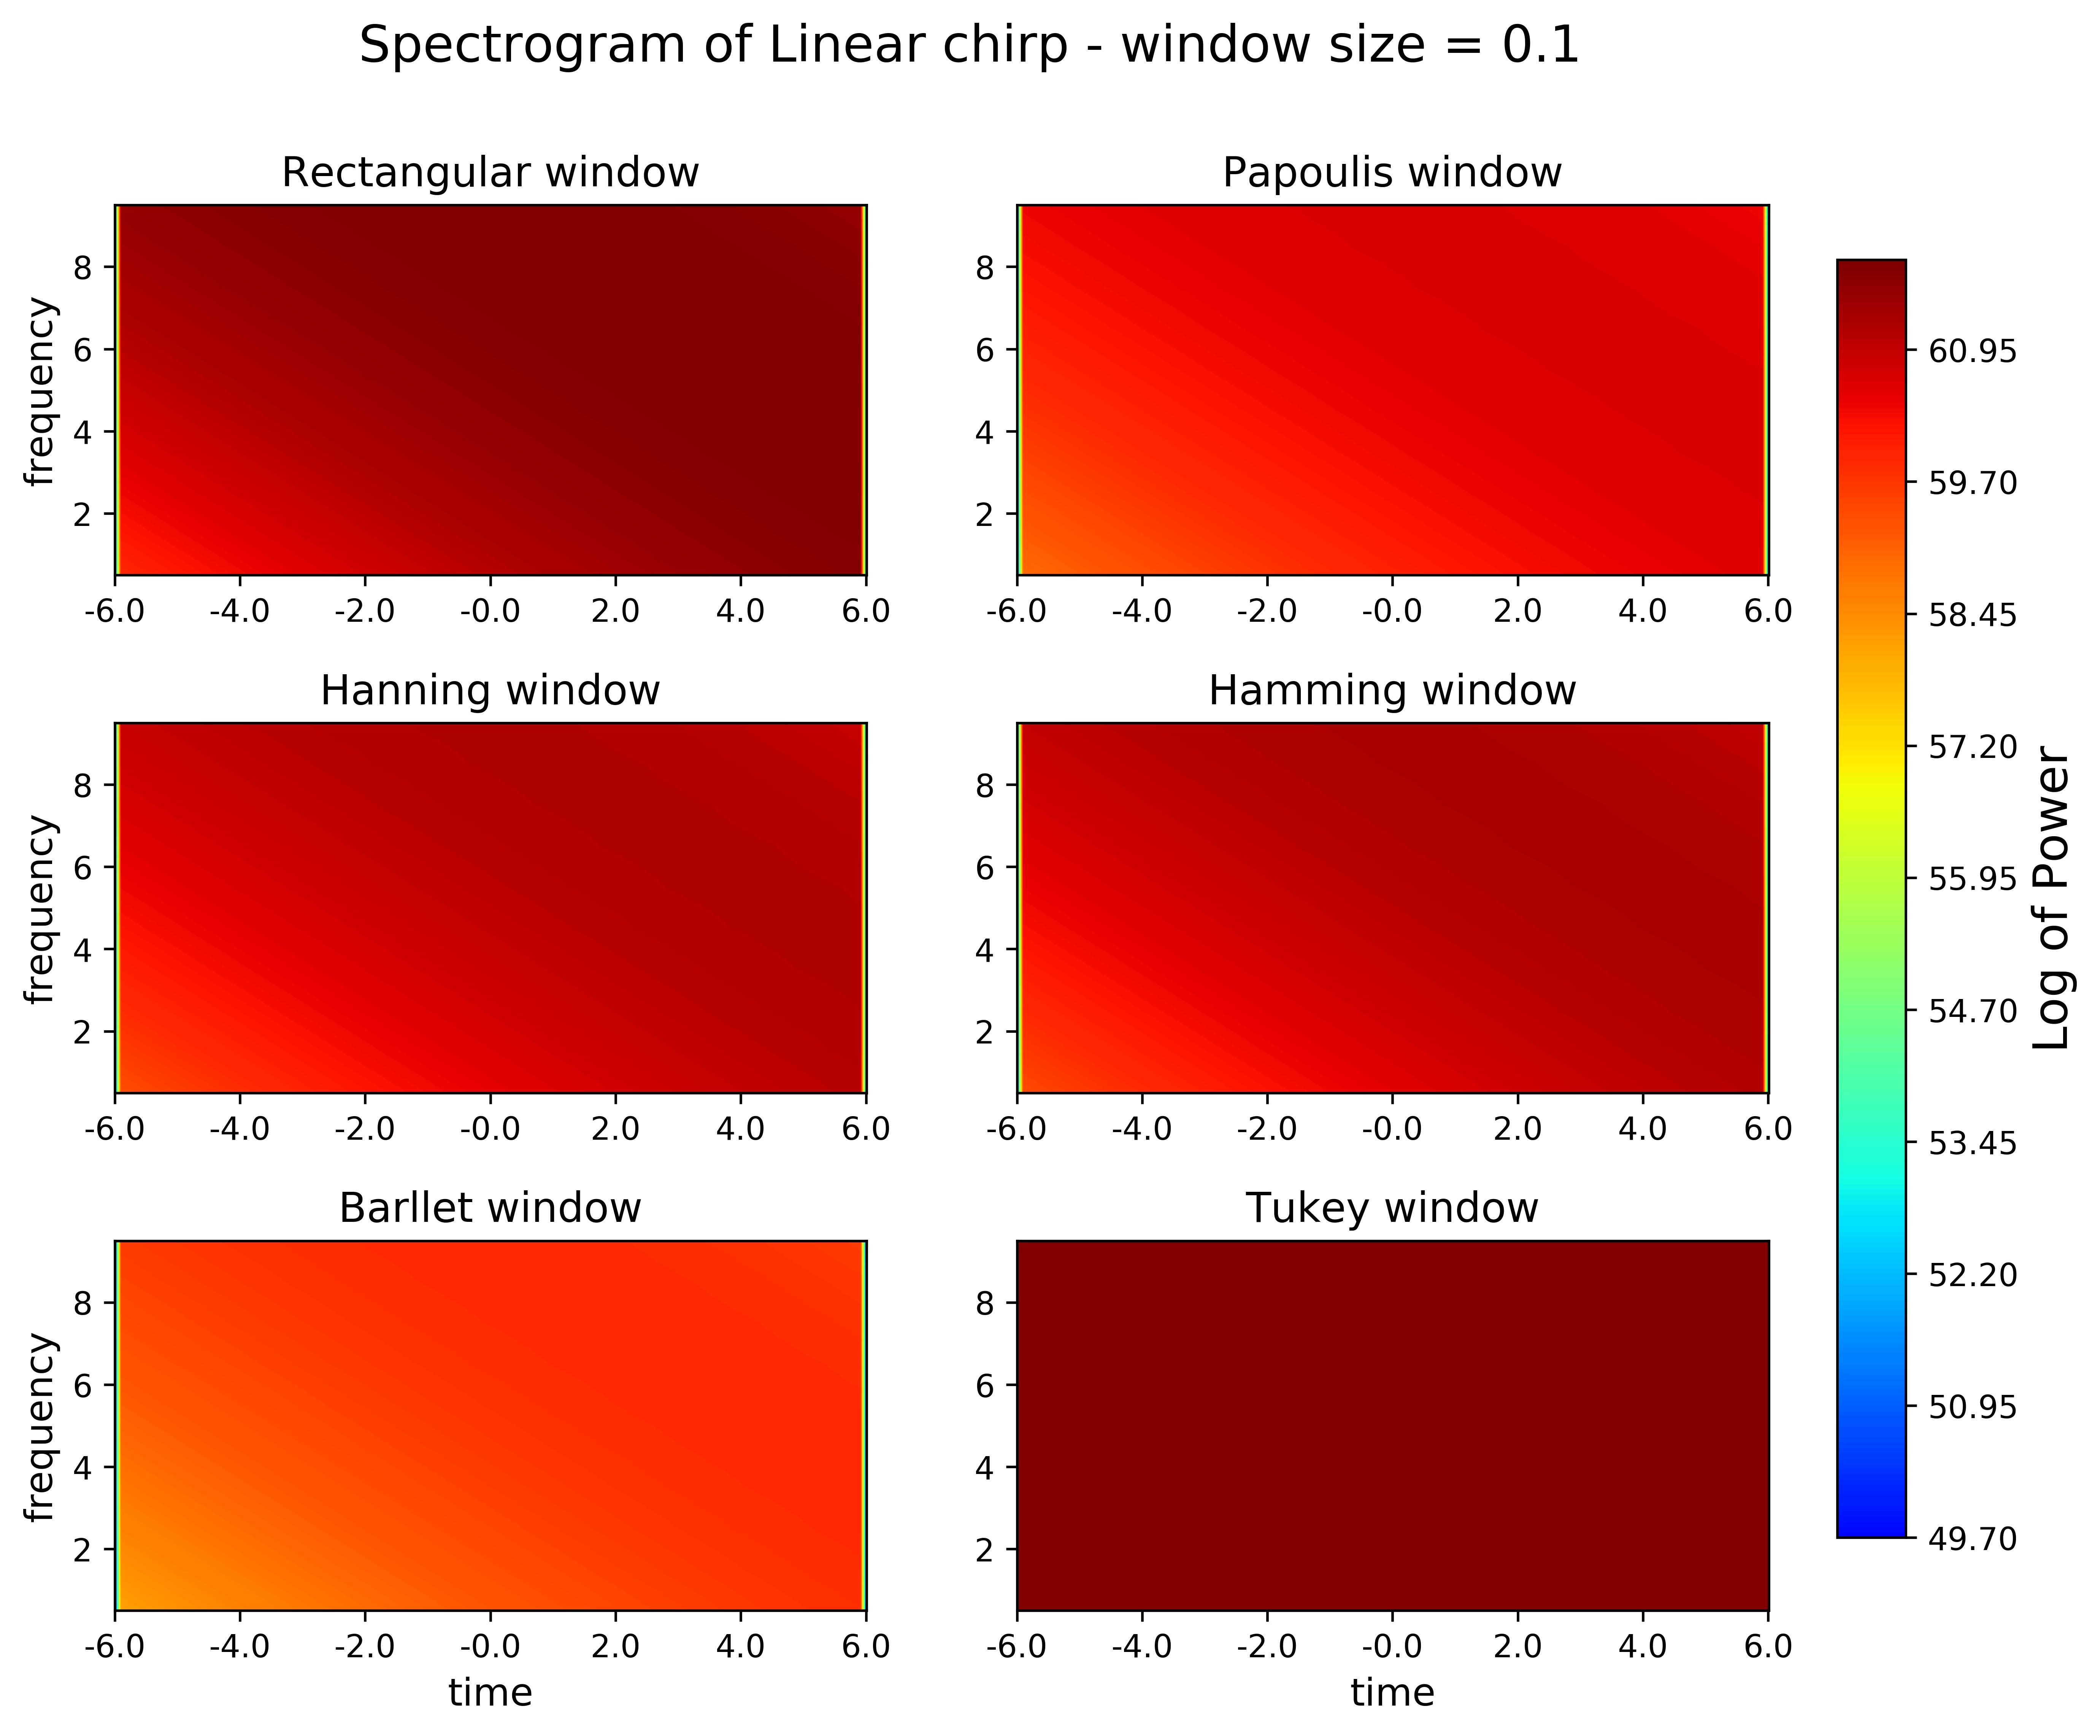
\includegraphics{../scripts/exercicio2/espectros/Linear_ws0.1.jpg}}	
	\end{center}
	\vspace{1mm}
	\label{ex1_fig1}
\end{figure}

Espectrogramas do \textbf{chirp linear}, $-6 \leq t \leq 6$ e tamanho das janelas = 0.5: Figura 2.8.

% FIGURA
\begin{figure}[ht!]
	\legenda{Figura 2.8: Espectrogramas do chirp linear com janelas de tamanho igual a 0.5. Comparar com segunda linha (de cima para baixo) da Figura 1.1.}
	\vspace{3mm}	
	\begin{center}
		\resizebox{\textwidth}{!}{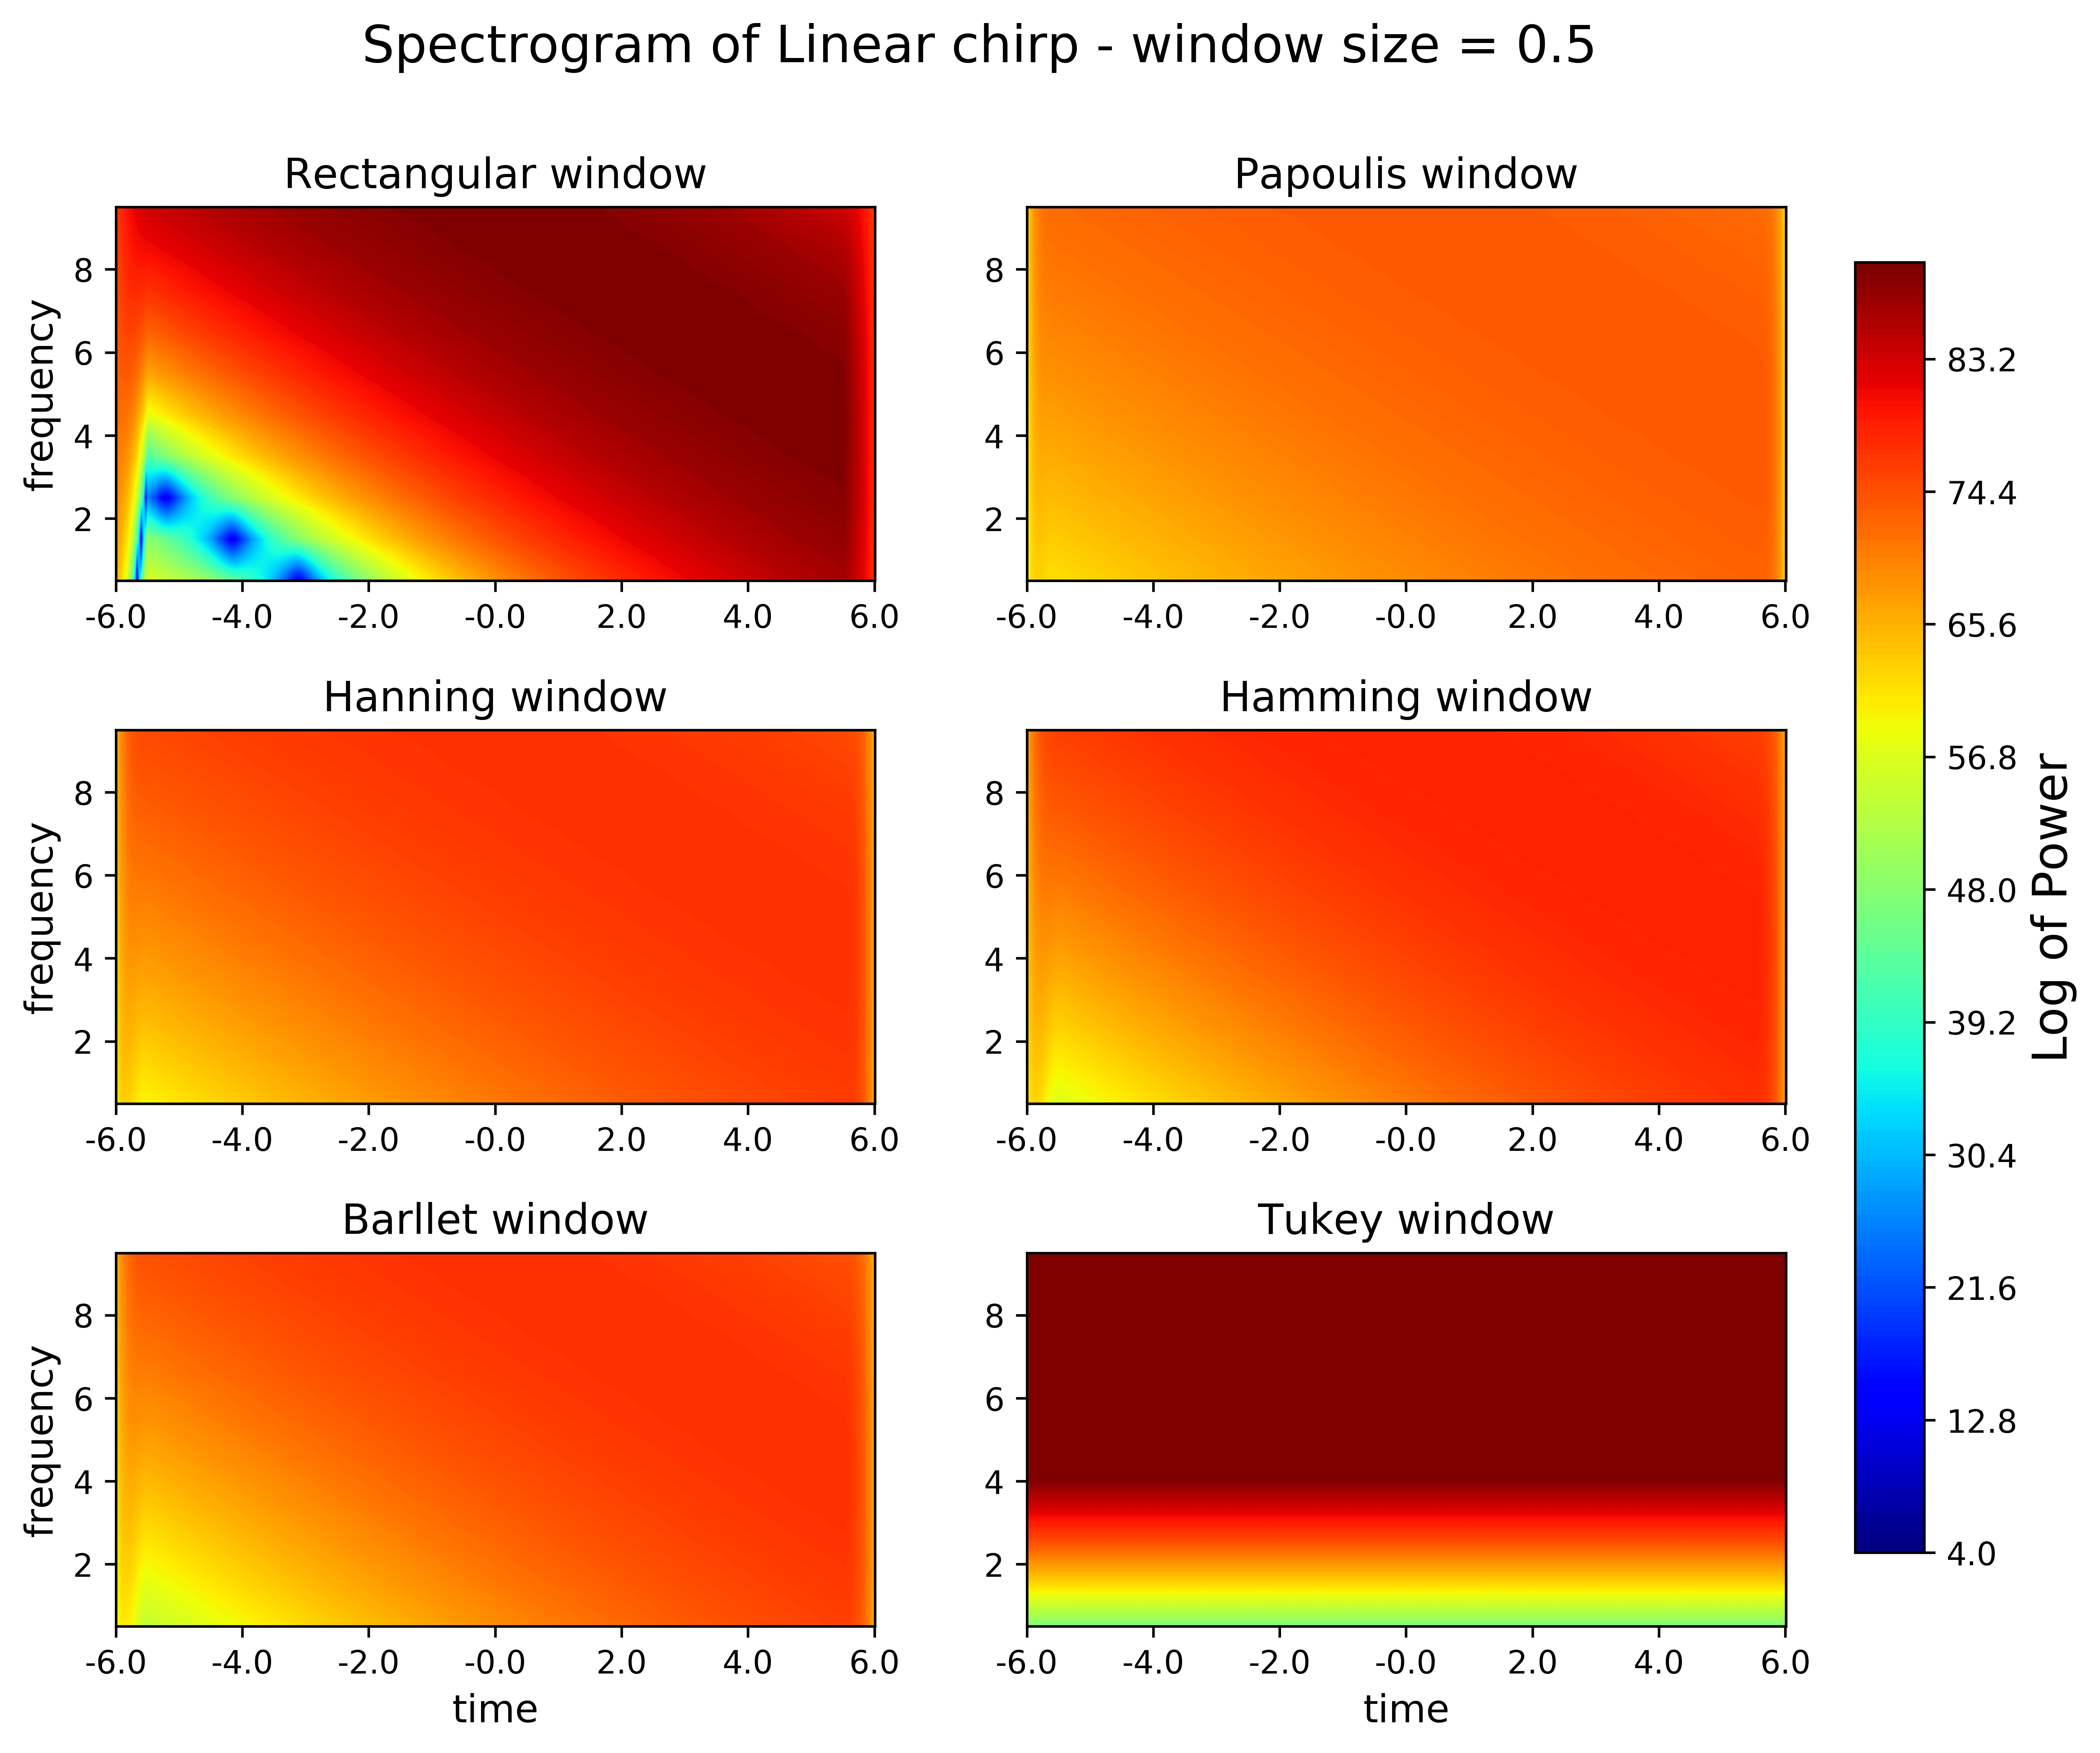
\includegraphics{../scripts/exercicio2/espectros/Linear_ws0.5.jpg}}	
	\end{center}
	\vspace{1mm}
	\label{ex1_fig1}
\end{figure}


Espectrogramas do \textbf{chirp linear}, $0 \leq t \leq 6$ e tamanho das janelas = 0.5: Figura 2.9.

% FIGURA
\begin{figure}[ht!]
	\legenda{Figura 2.9: Espectrogramas do chirp linear com janelas de tamanho igual a 0.5. Comparar com segunda linha (de cima para baixo) da Figura 1.3.}
	\vspace{3mm}	
	\begin{center}
		\resizebox{\textwidth}{!}{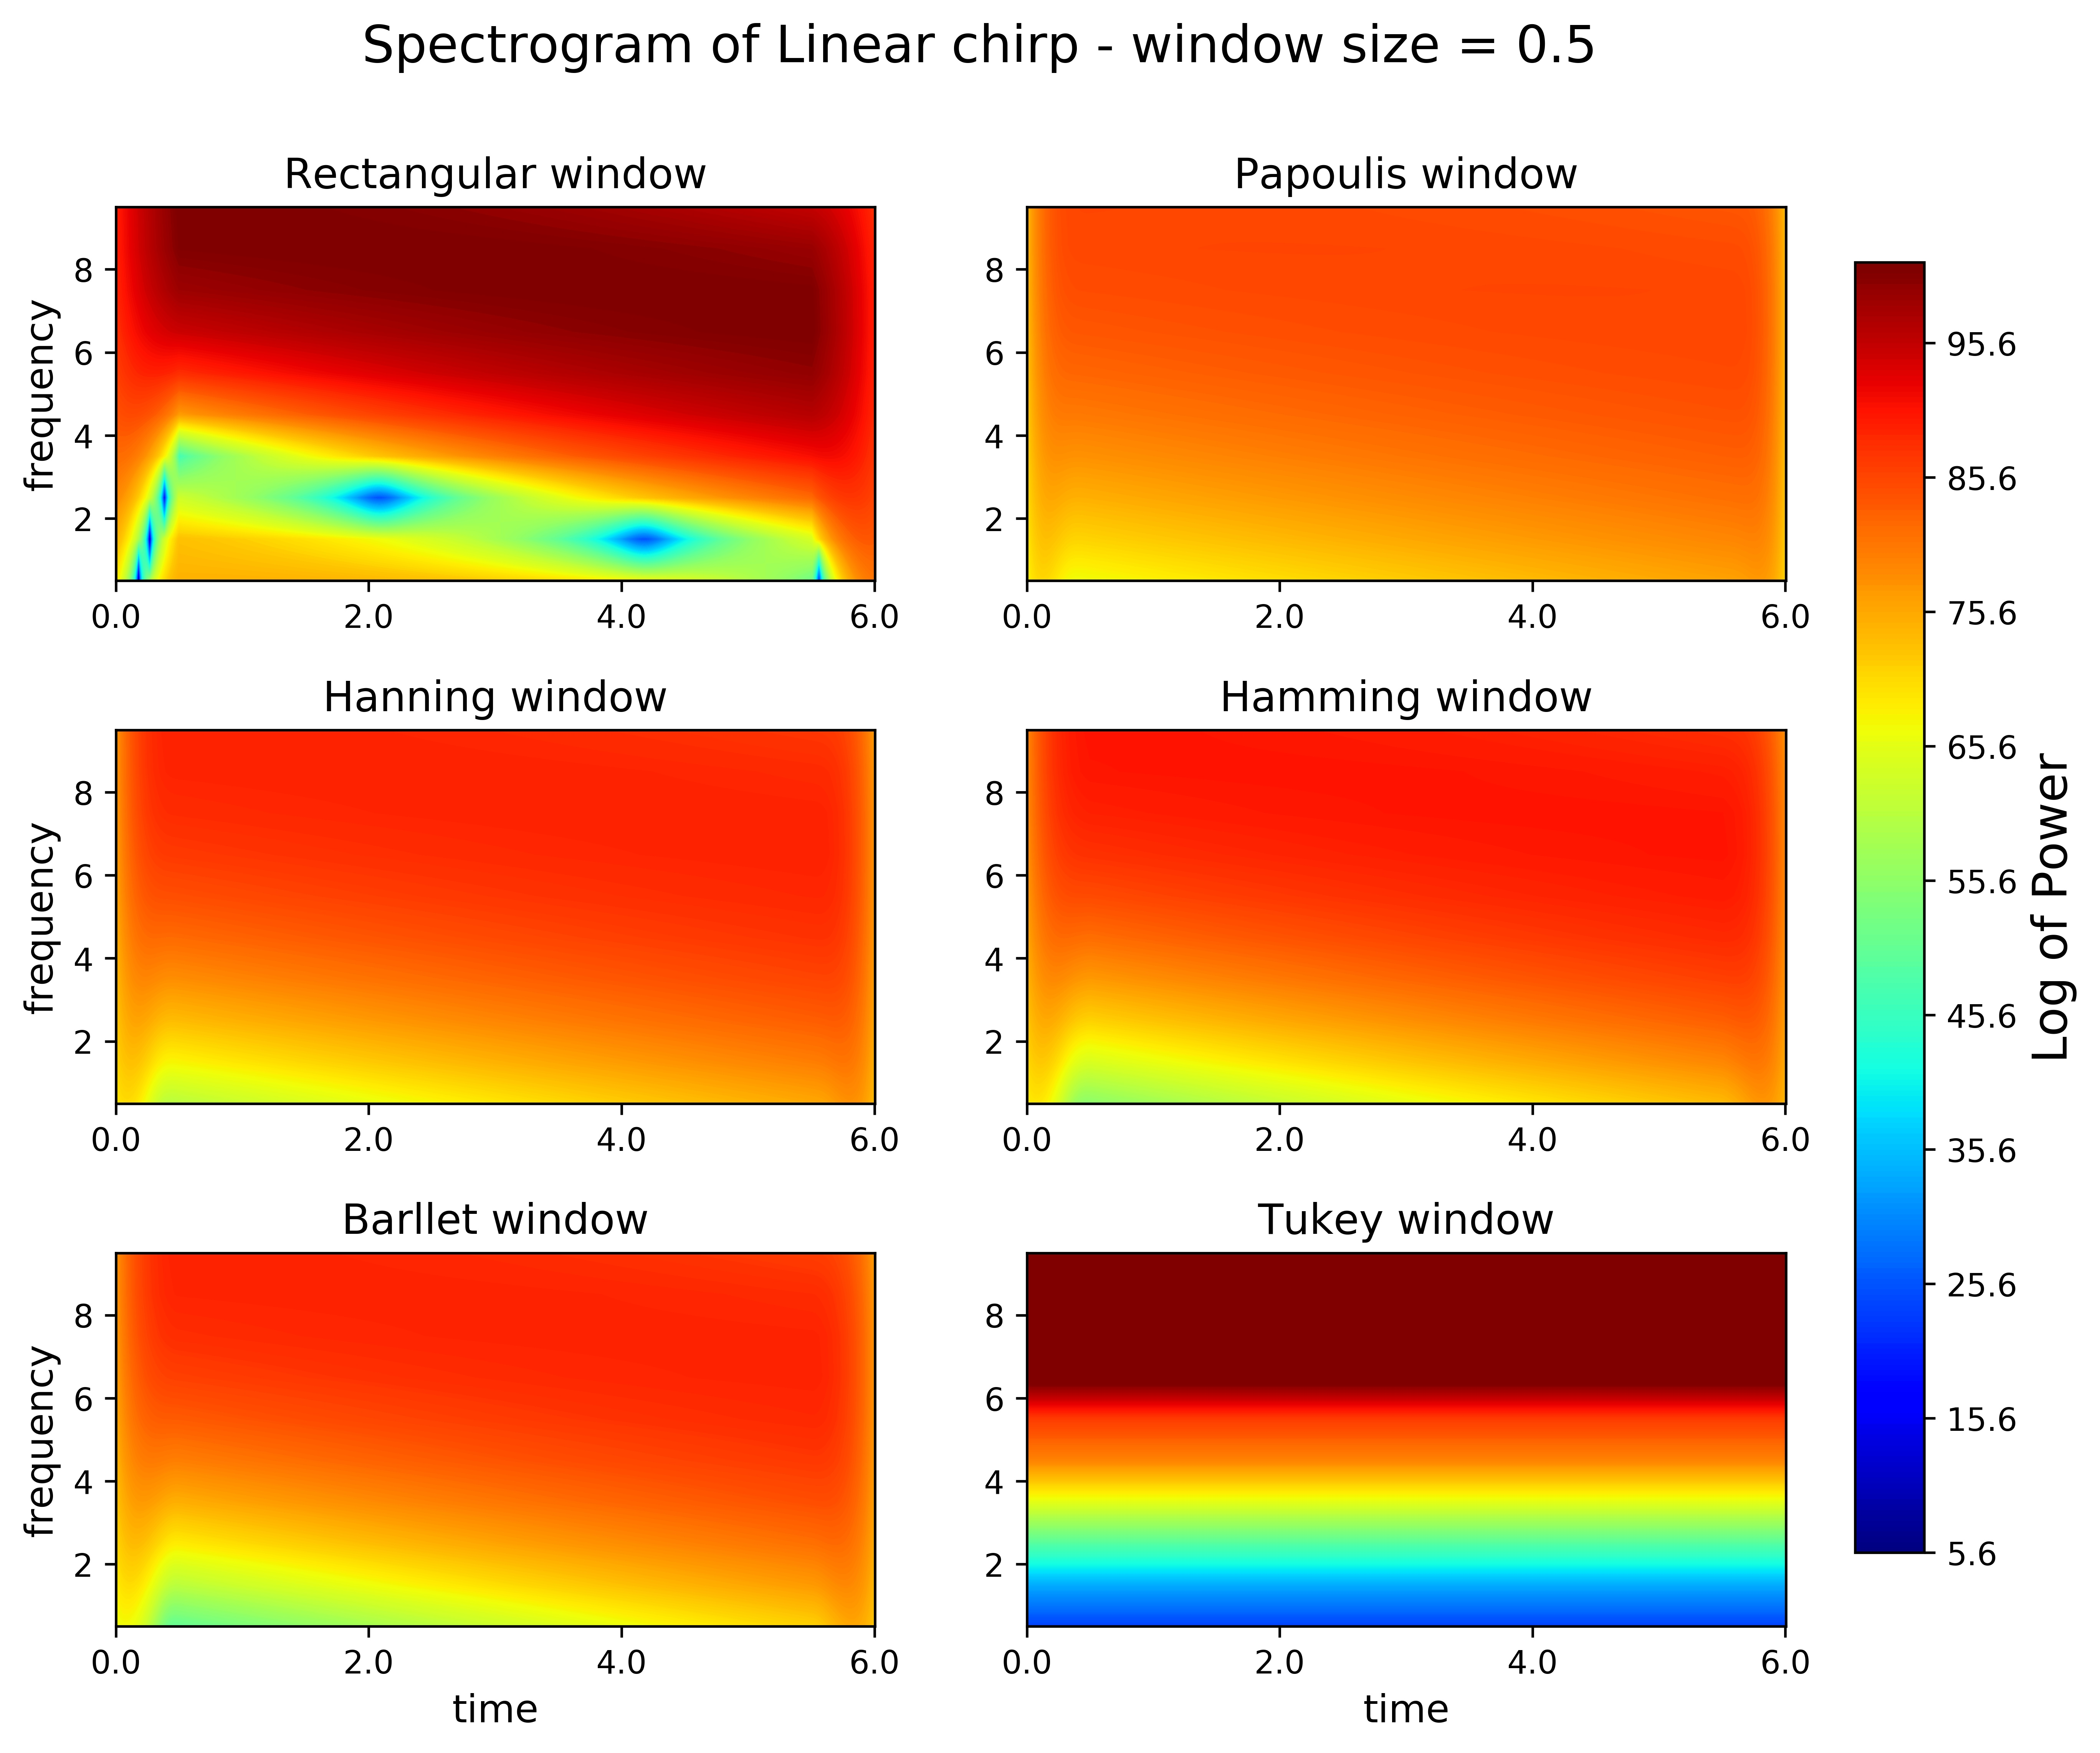
\includegraphics{../scripts/exercicio2/espectros/TEST_Linear_ws0.5.jpg}}	
	\end{center}
	\vspace{1mm}
	\label{ex1_fig1}
\end{figure}

%%%%%%%%%%%%%%%% Quadratic


Espectrogramas do \textbf{chirp quadrático}, $-4 \leq t \leq 4$ e tamanho das janelas = 0.1: Figura 2.10.

% FIGURA
\begin{figure}[ht!]
	\legenda{Figura 2.10: Espectrogramas do chirp quadrático com janelas de tamanho igual a 0.1. Comparar com terceira linha (de cima para baixo) da Figura 1.1.}
	\vspace{3mm}	
	\begin{center}
		\resizebox{\textwidth}{!}{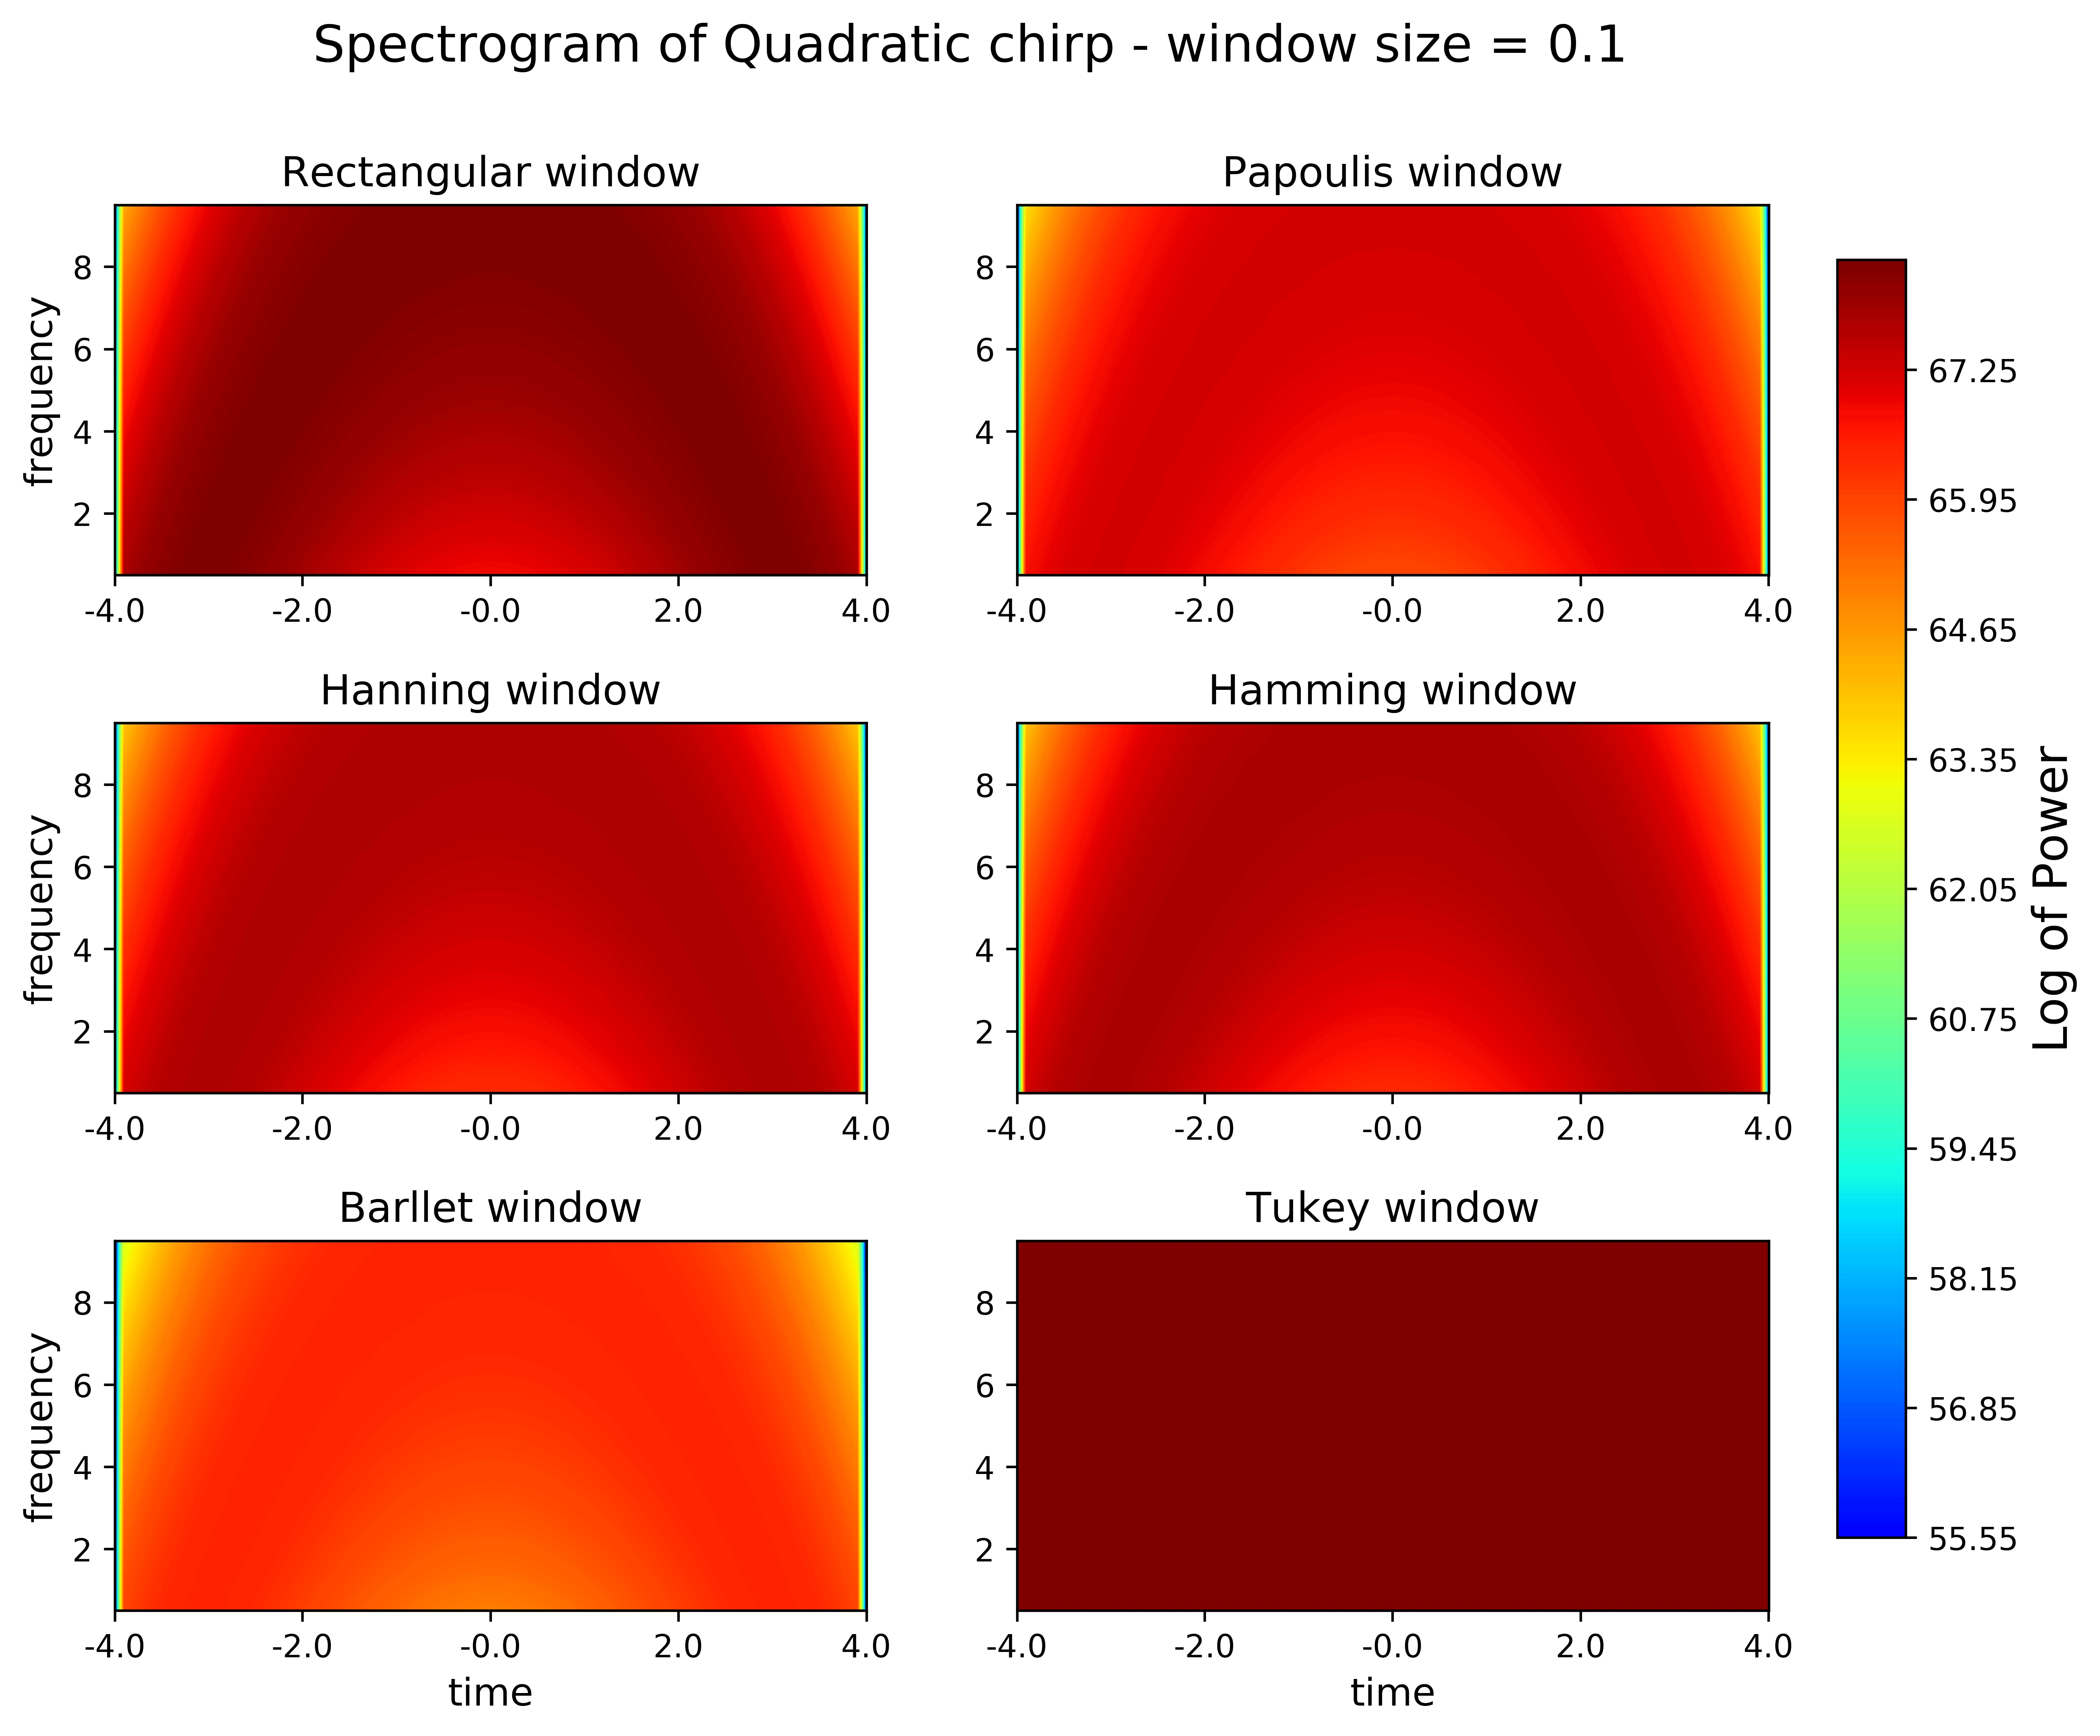
\includegraphics{../scripts/exercicio2/espectros/Quadratic_ws0.1.jpg}}	
	\end{center}
	\vspace{1mm}
	\label{ex1_fig1}
\end{figure}

Espectrogramas do \textbf{chirp quadrático}, $-4 \leq t \leq 4$ e tamanho das janelas = 0.5: Figura 2.11.

% FIGURA
\begin{figure}[ht!]
	\legenda{Figura 2.11: Espectrogramas do chirp quadrático com janelas de tamanho igual a 0.5. Comparar com terceira linha (de cima para baixo) da Figura 1.1.}
	\vspace{3mm}	
	\begin{center}
		\resizebox{\textwidth}{!}{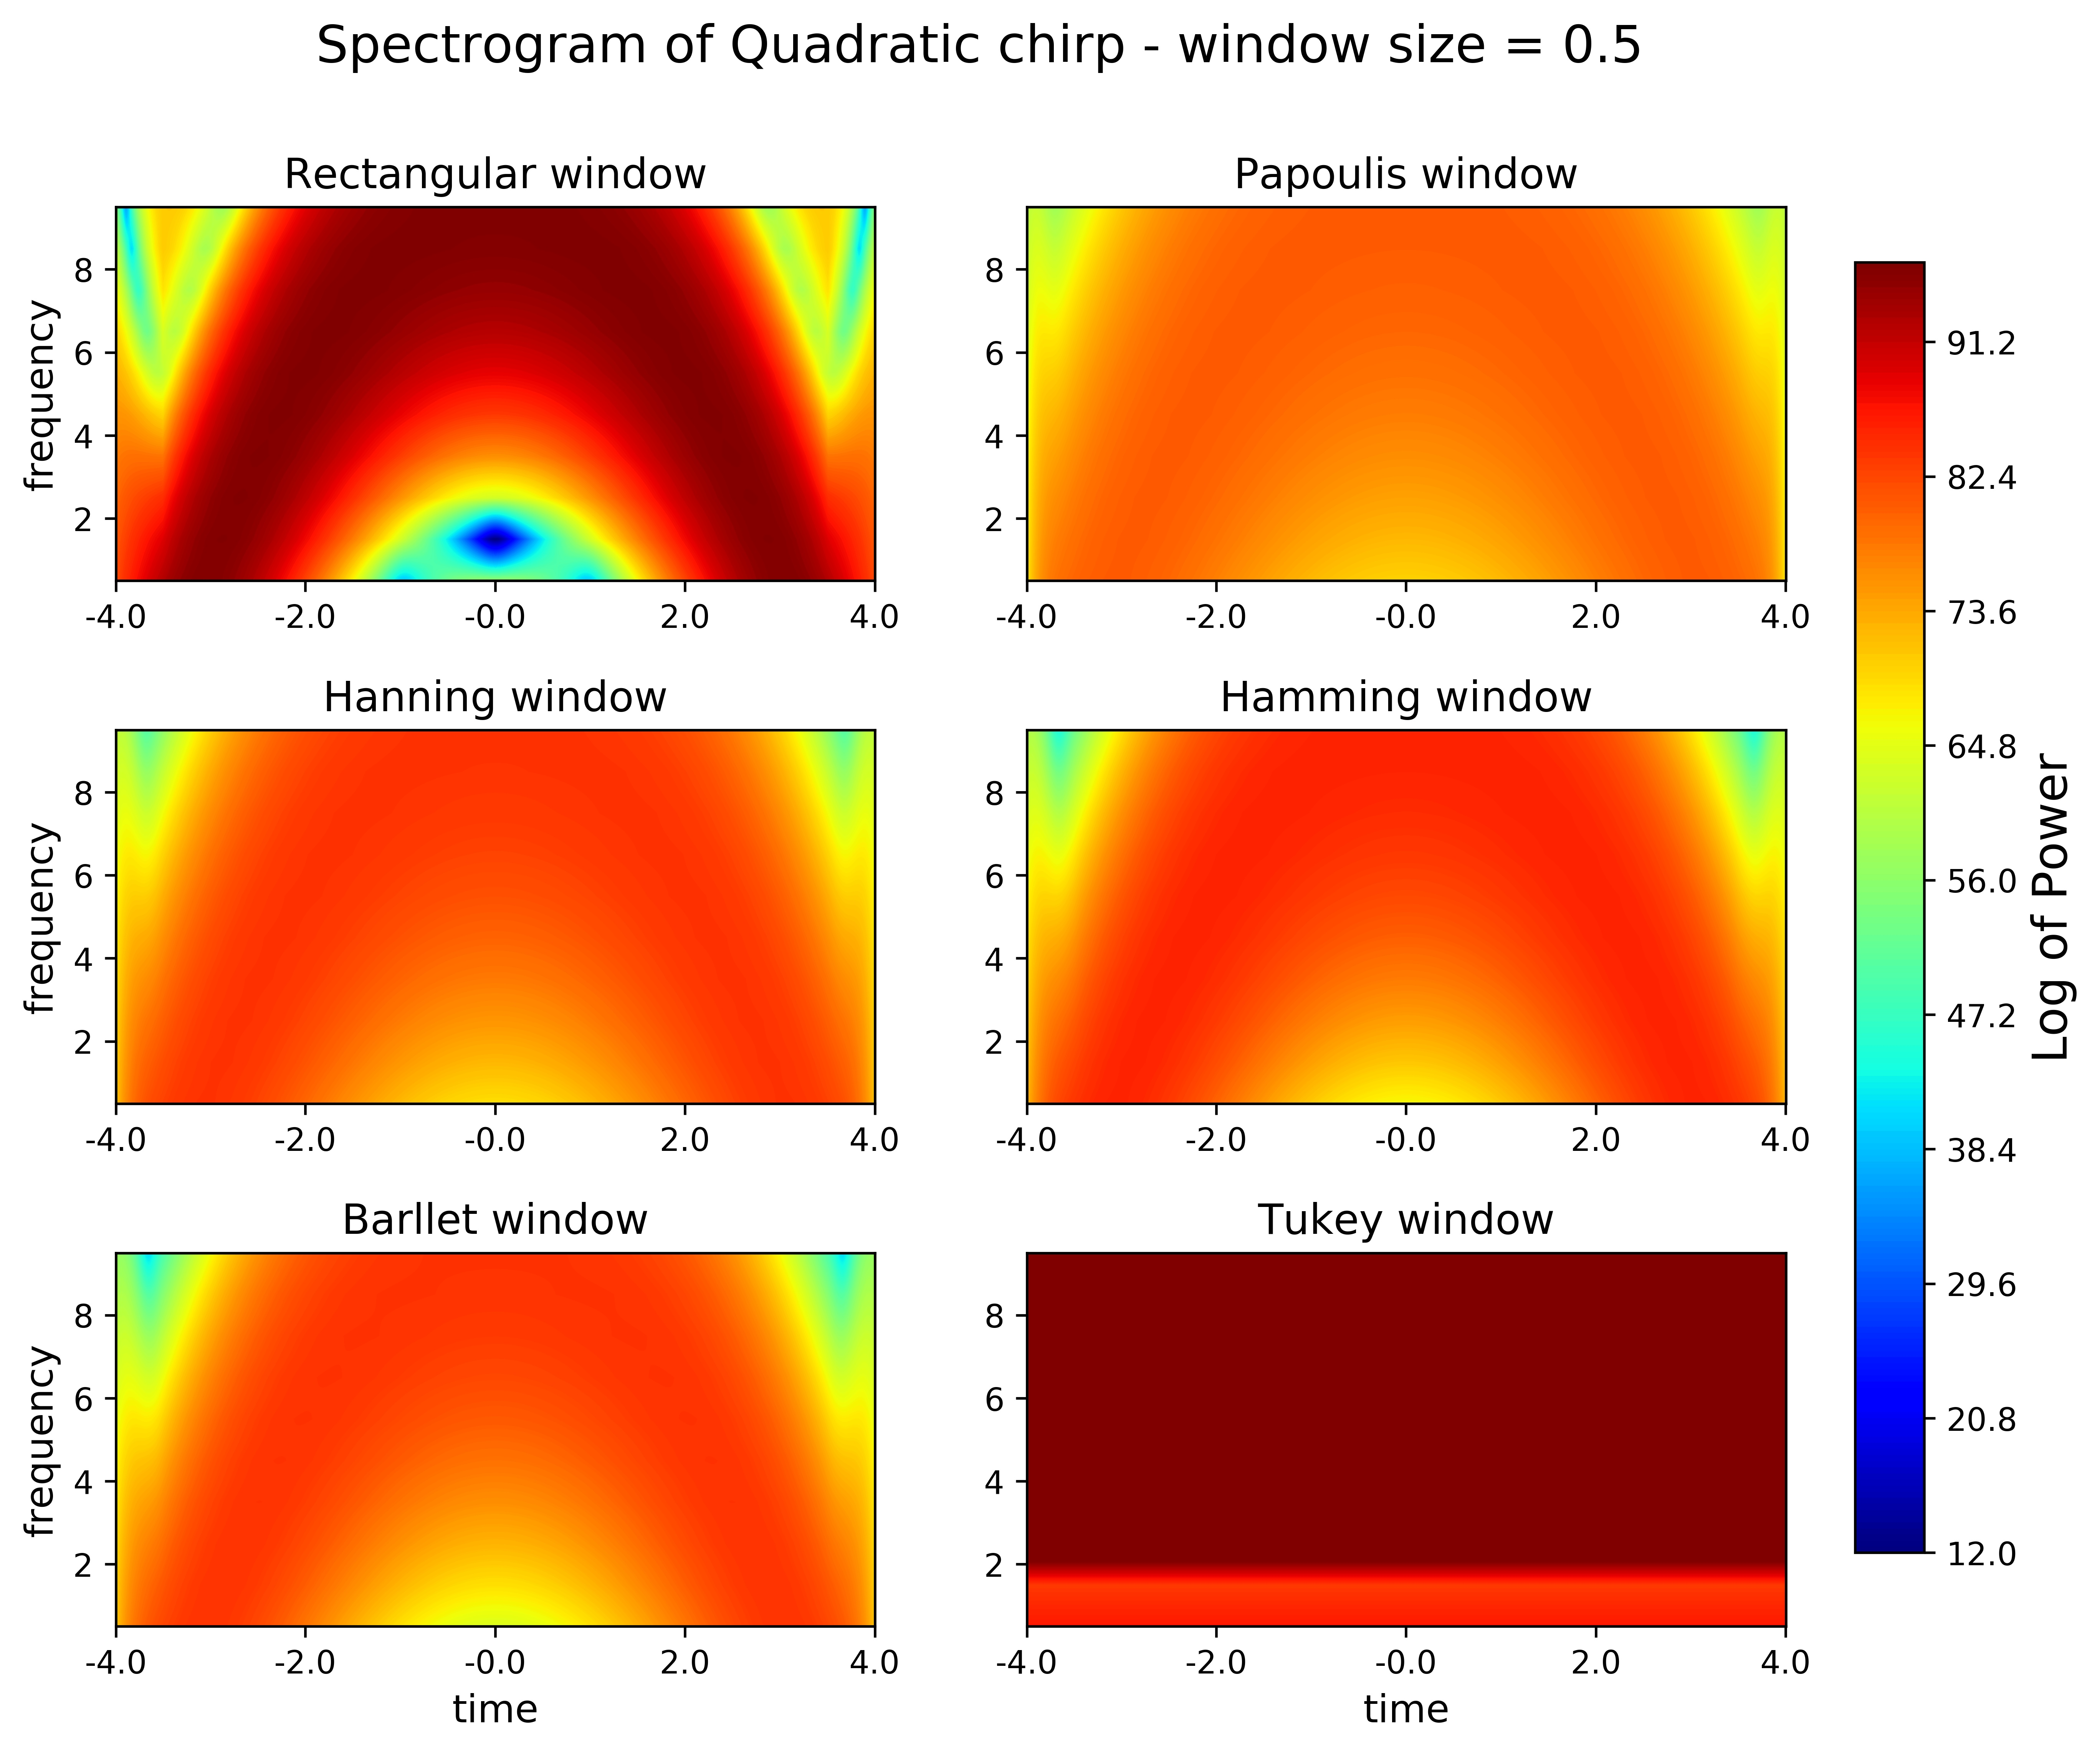
\includegraphics{../scripts/exercicio2/espectros/Quadratic_ws0.5.jpg}}	
	\end{center}
	\vspace{1mm}
	\label{ex1_fig1}
\end{figure}


Espectrogramas do \textbf{chirp quadrático}, $0 \leq t \leq 6$ e tamanho das janelas = 0.5: Figura 2.12.

% FIGURA
\begin{figure}[ht!]
	\legenda{Figura 2.12: Espectrogramas do chirp quadrático com janelas de tamanho igual a 0.5. Comparar com terceira linha (de cima para baixo) da Figura 1.3.}
	\vspace{3mm}	
	\begin{center}
		\resizebox{\textwidth}{!}{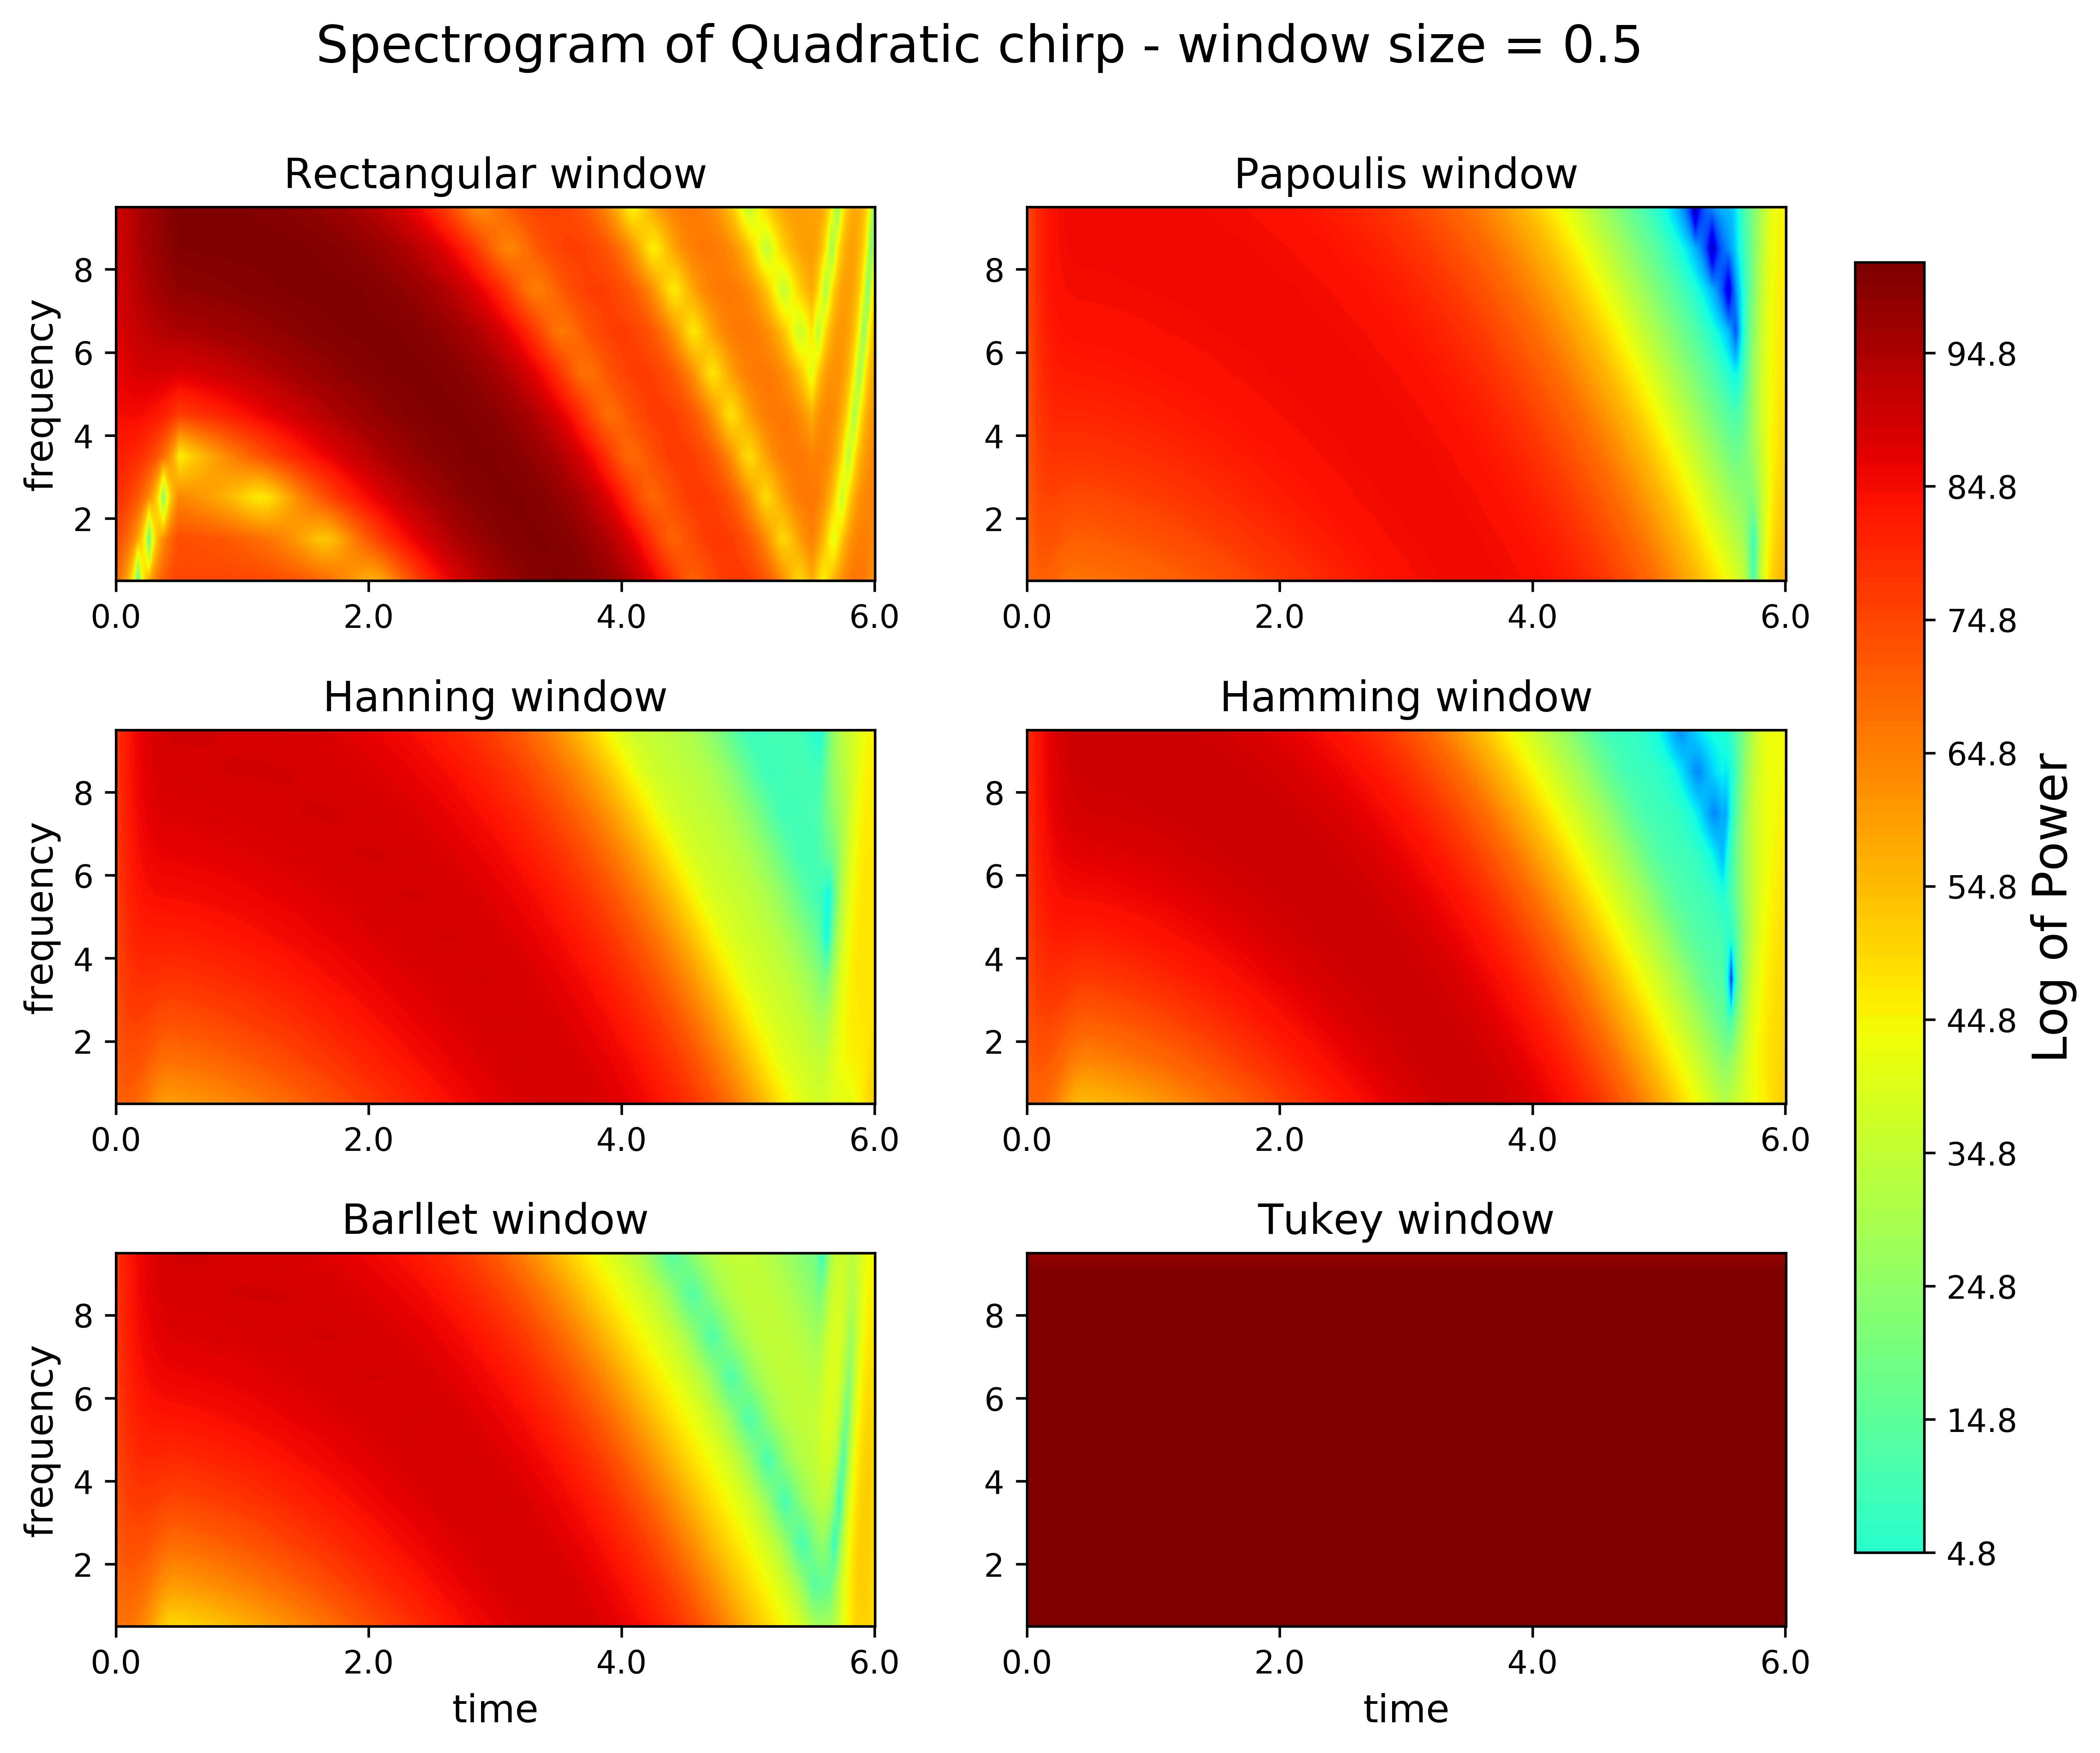
\includegraphics{../scripts/exercicio2/espectros/TEST_Quadratic_ws0.5.jpg}}	
	\end{center}
	\vspace{1mm}
	\label{ex1_fig1}
\end{figure}


%%%%%%%%%%%%%%%% Hyperbolic


Espectrogramas do \textbf{chirp hiperbólico}, $0 \leq t \leq 2$ e tamanho das janelas = 0.1: Figura 2.13.

% FIGURA
\begin{figure}[ht!]
	\legenda{Figura 2.13: Espectrogramas do chirp hiperbólico com janelas de tamanho igual a 0.1. Comparar com última linha da Figura 1.1.}
	\vspace{3mm}	
	\begin{center}
		\resizebox{\textwidth}{!}{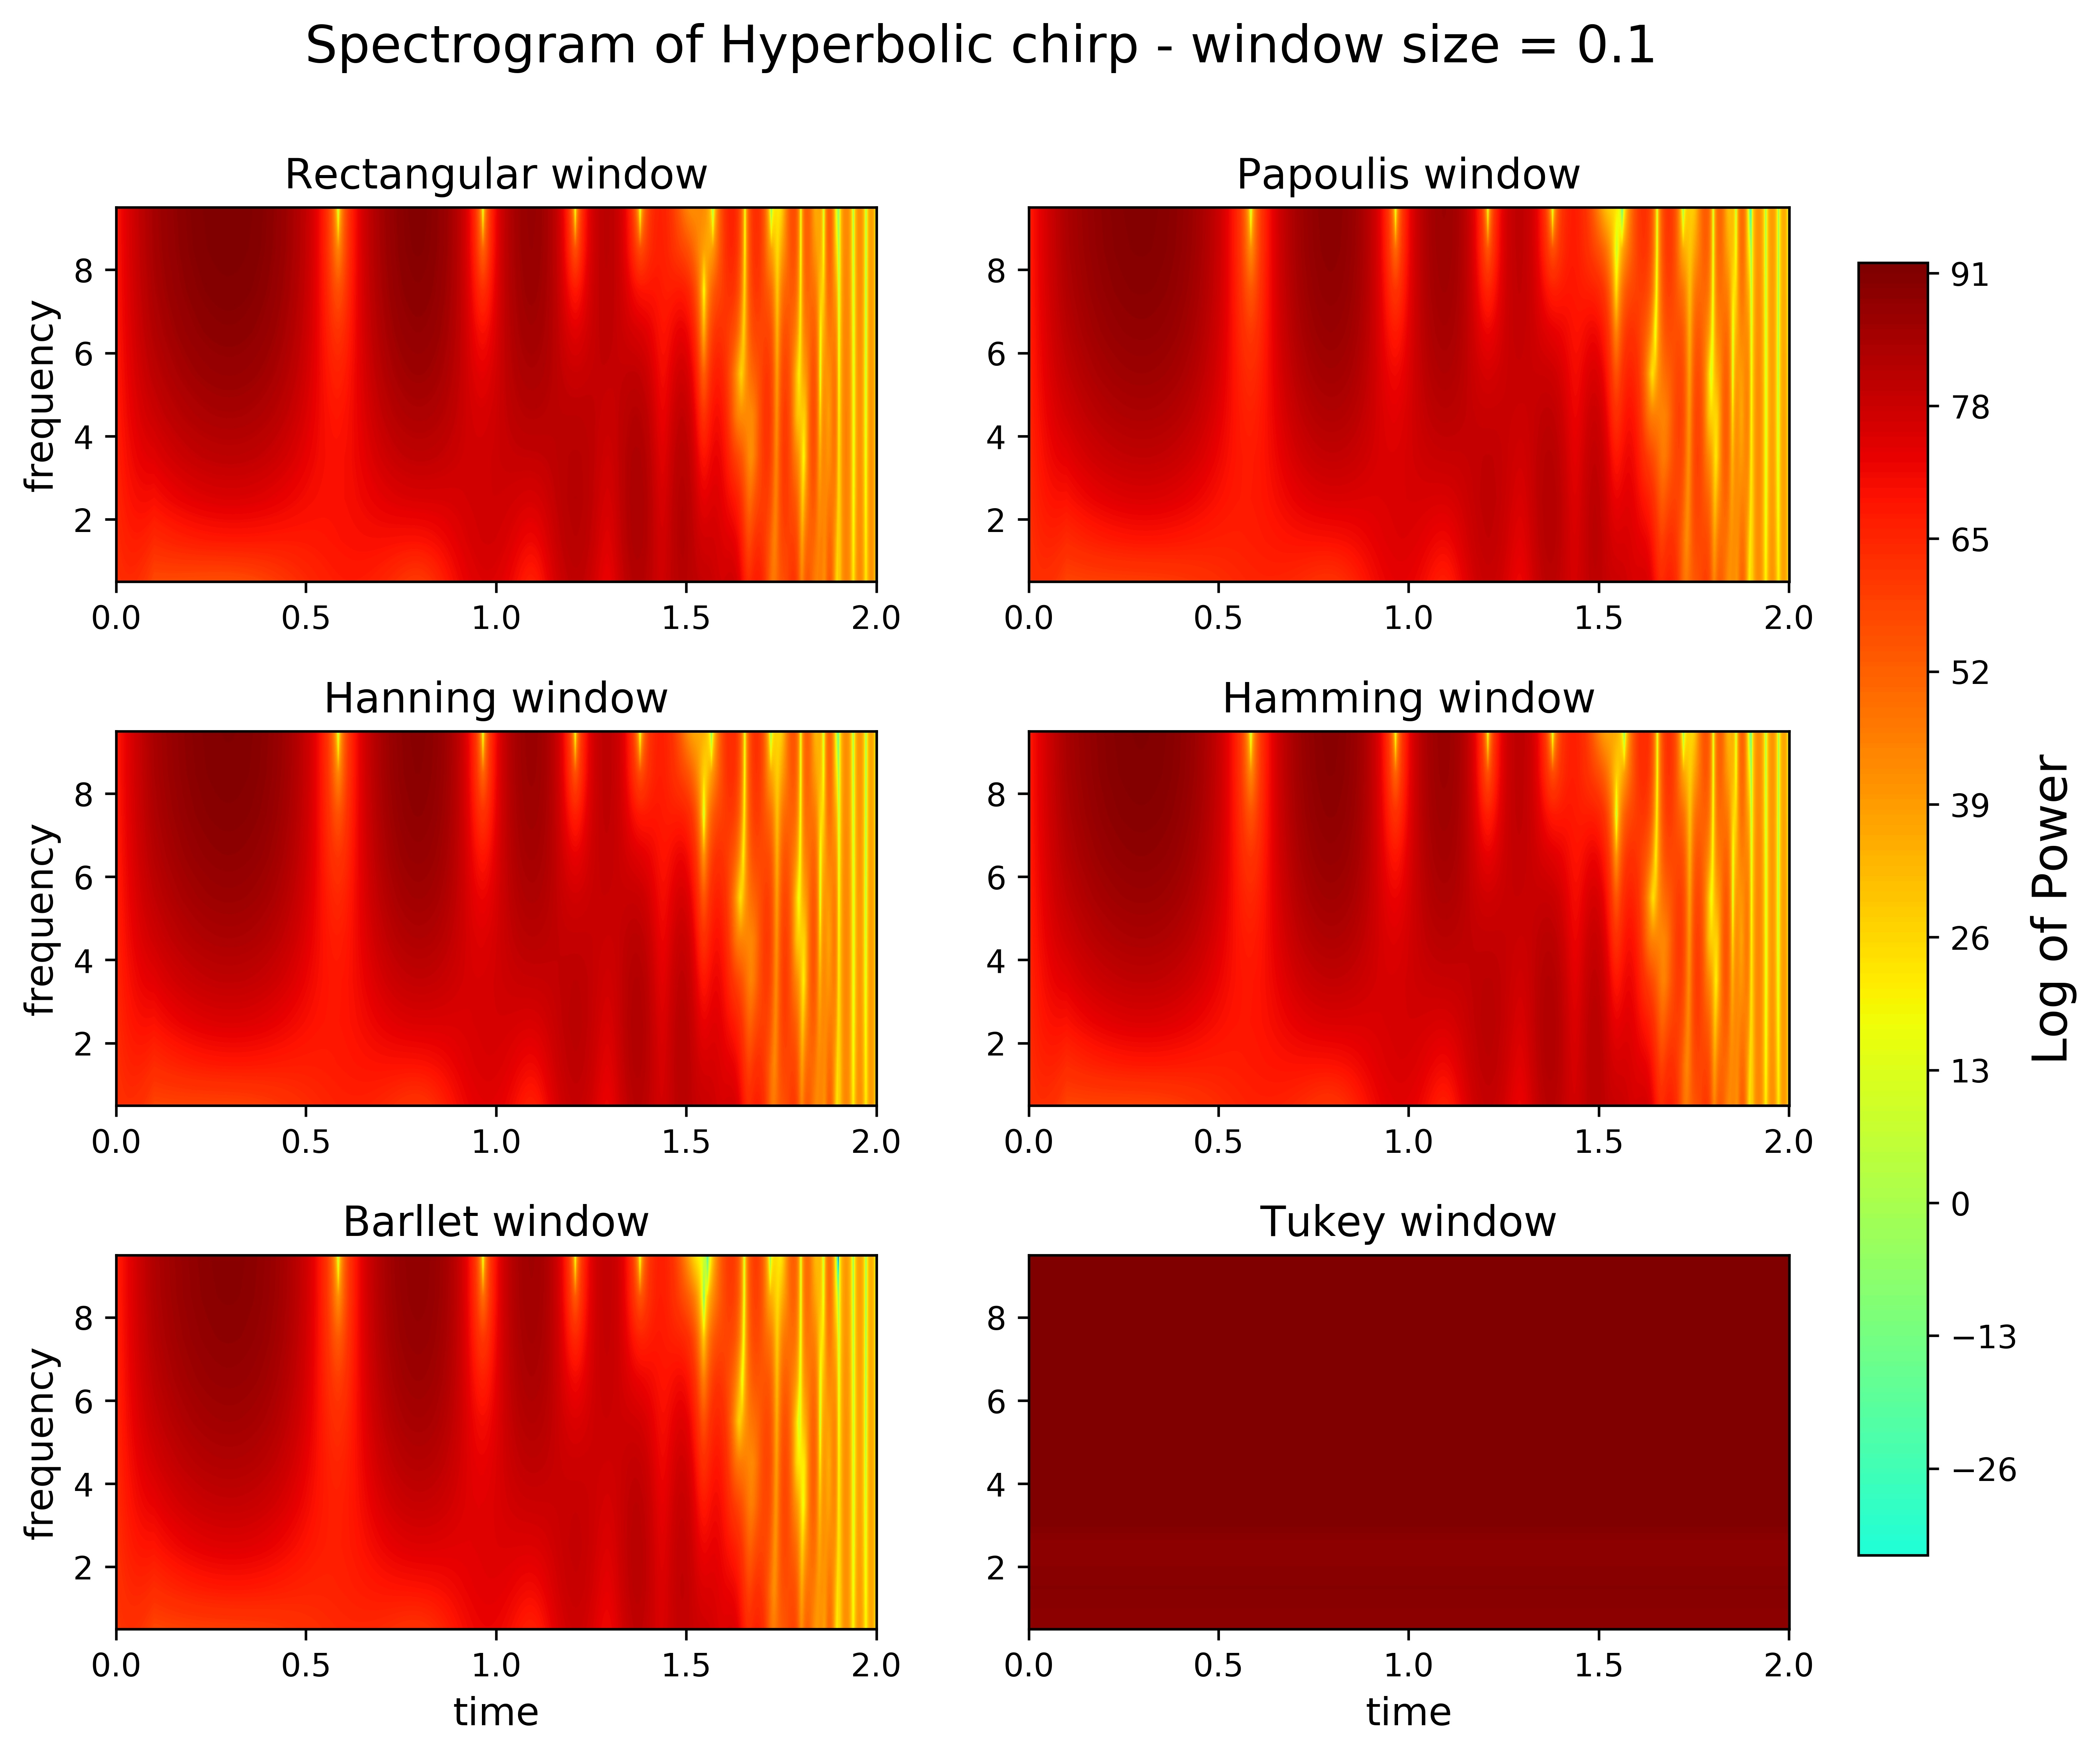
\includegraphics{../scripts/exercicio2/espectros/Hyperbolic_ws0.1.jpg}}	
	\end{center}
	\vspace{1mm}
	\label{ex1_fig1}
\end{figure}

Espectrogramas do \textbf{chirp hiperbólico}, $0 \leq t \leq 2$ e tamanho das janelas = 0.5: Figura 2.14.

% FIGURA
\begin{figure}[ht!]
	\legenda{Figura 2.14: Espectrogramas do chirp hiperbólico com janelas de tamanho igual a 0.5. Comparar com última linha da Figura 1.1.}
	\vspace{3mm}	
	\begin{center}
		\resizebox{\textwidth}{!}{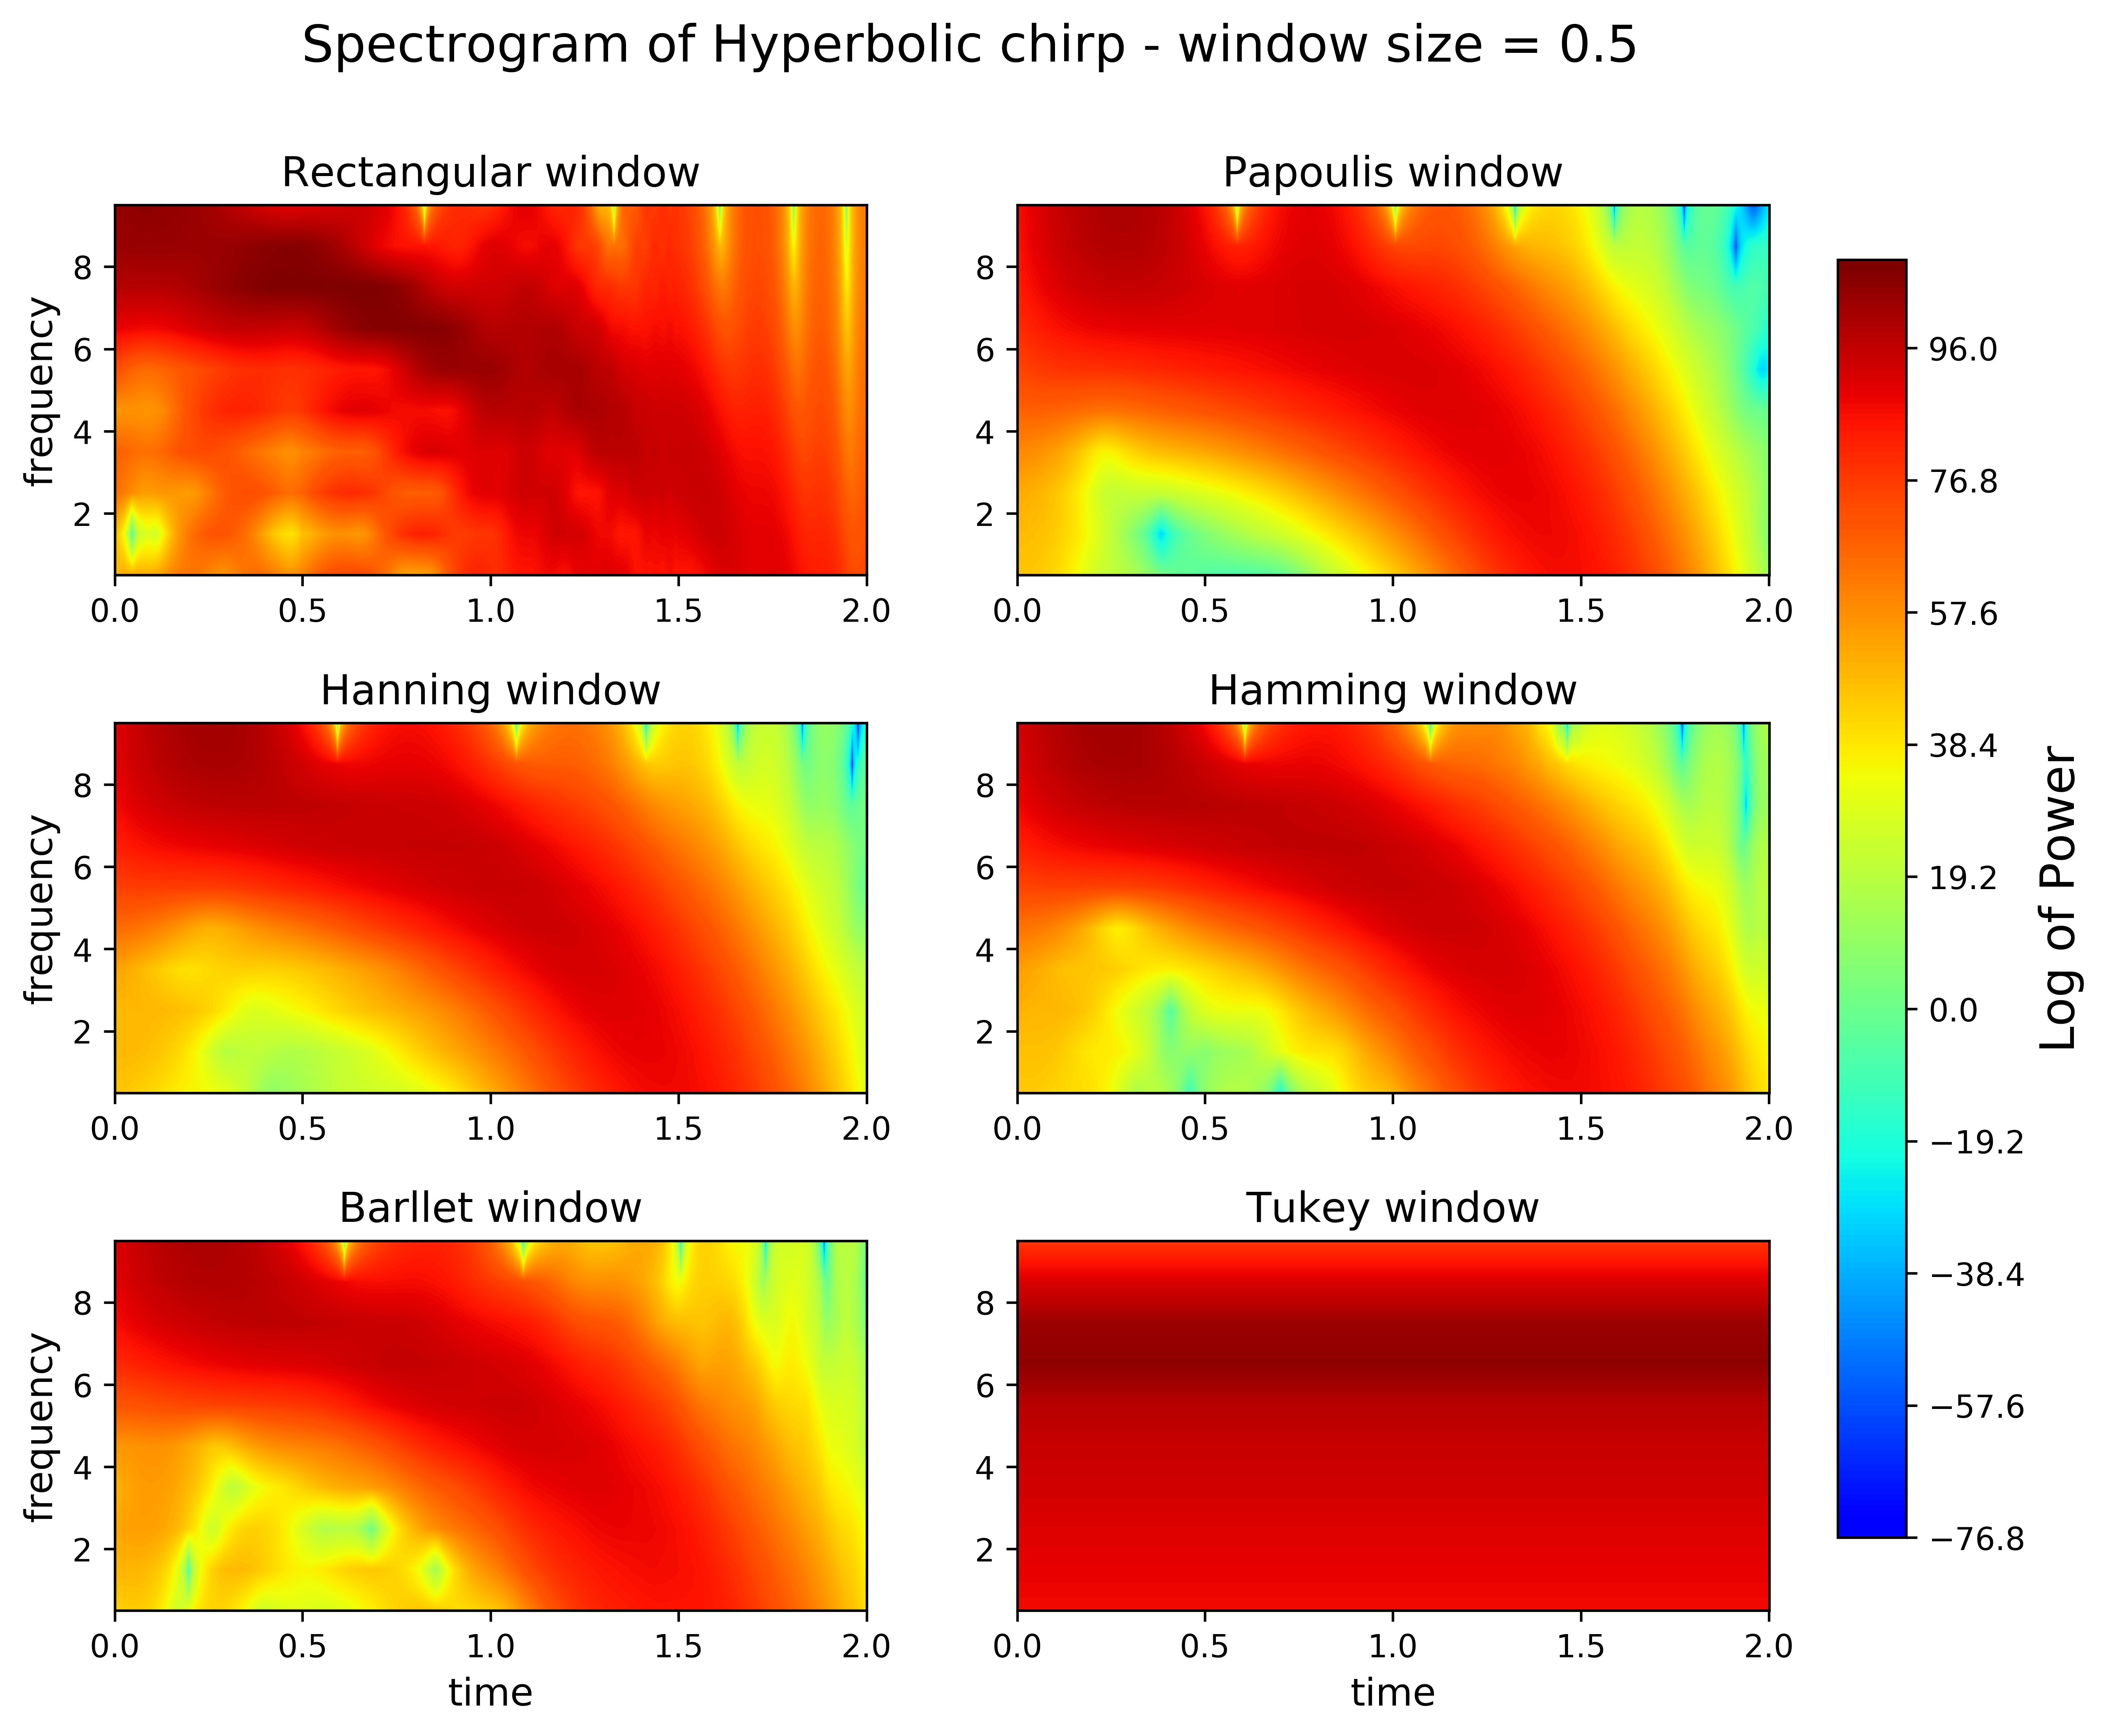
\includegraphics{../scripts/exercicio2/espectros/Hyperbolic_ws0.5.jpg}}	
	\end{center}
	\vspace{1mm}
	\label{ex1_fig1}
\end{figure}

Espectrogramas do \textbf{chirp hiperbólico}, $0 \leq t \leq 6$ e tamanho das janelas = 0.1: Figura 2.15.

% FIGURA
\begin{figure}[ht!]
	\legenda{Figura 2.15: Espectrogramas do chirp hiperbólico com janelas de tamanho igual a 0.1. Comparar com última linha da Figura 1.3.}
	\vspace{3mm}	
	\begin{center}
		\resizebox{\textwidth}{!}{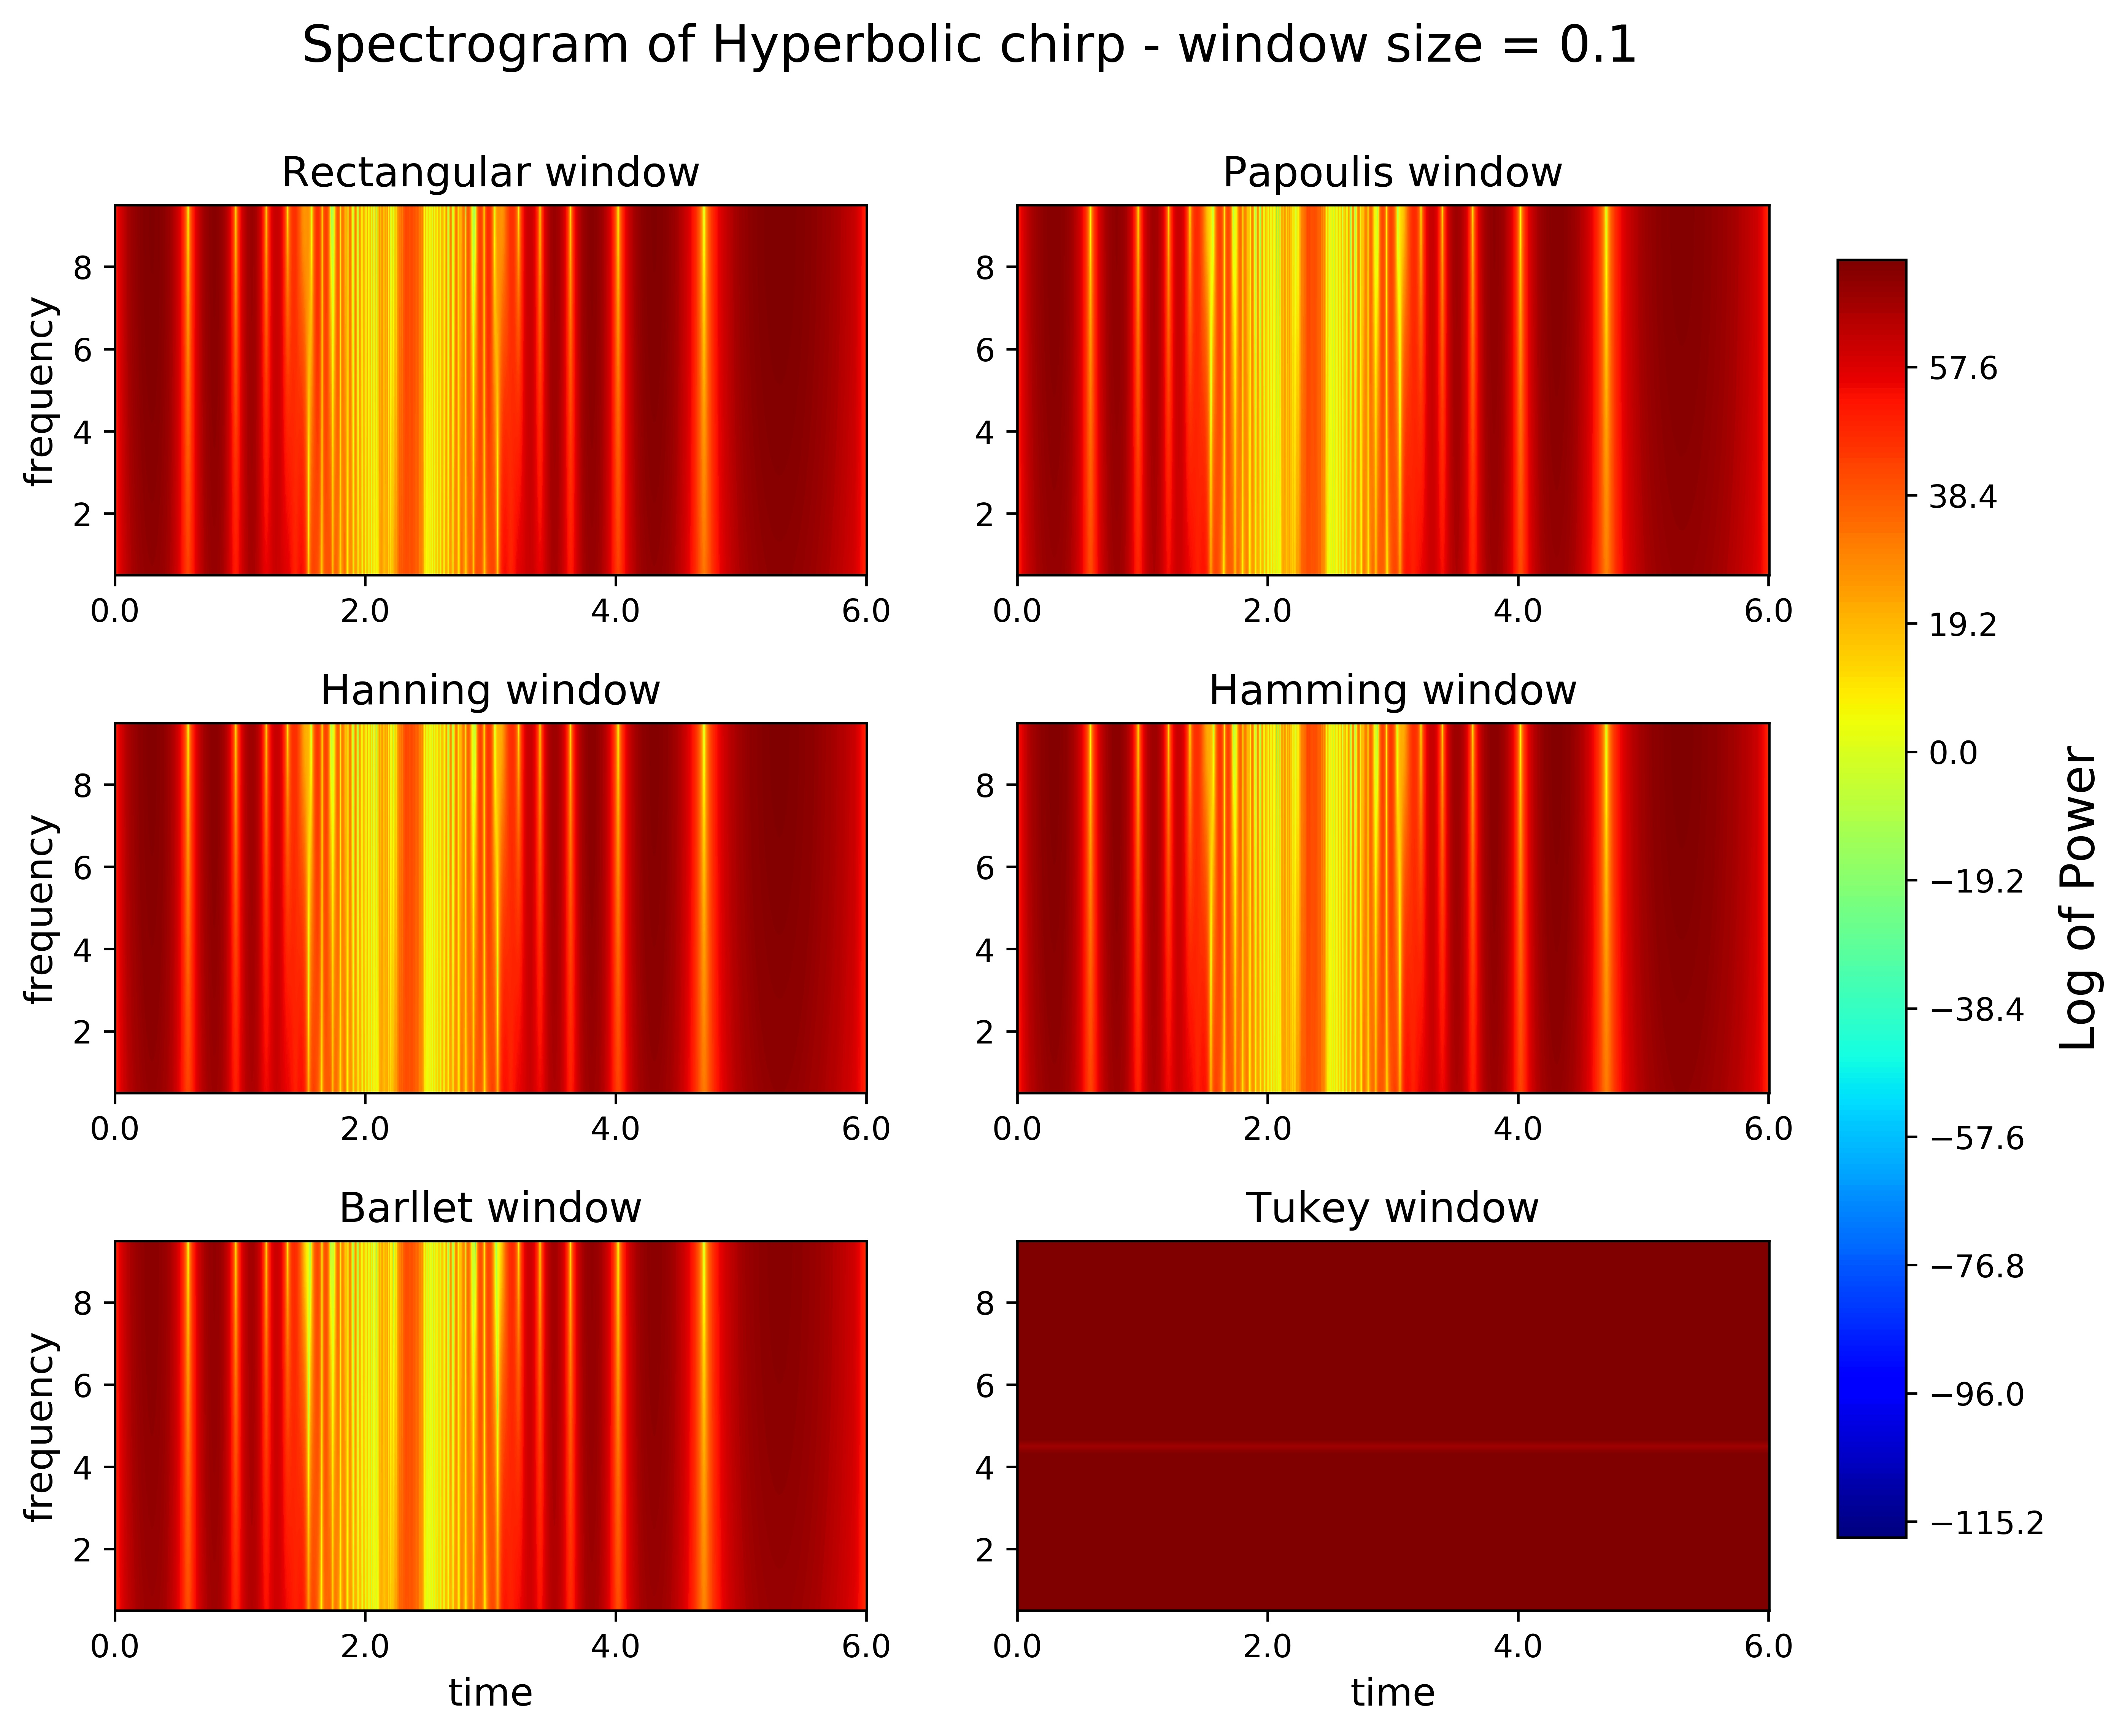
\includegraphics{../scripts/exercicio2/espectros/TEST_Hyperbolic_ws0.1.jpg}}	
	\end{center}
	\vspace{1mm}
	\label{ex1_fig1}
\end{figure}


Espectrogramas do \textbf{chirp hiperbólico}, $0 \leq t \leq 6$ e tamanho das janelas = 0.5: Figura 2.16.

% FIGURA
\begin{figure}[ht!]
	\legenda{Figura 2.16: Espectrogramas do chirp hiperbólico com janelas de tamanho igual a 0.5. Comparar com última linha da Figura 1.3.}
	\vspace{3mm}	
	\begin{center}
		\resizebox{\textwidth}{!}{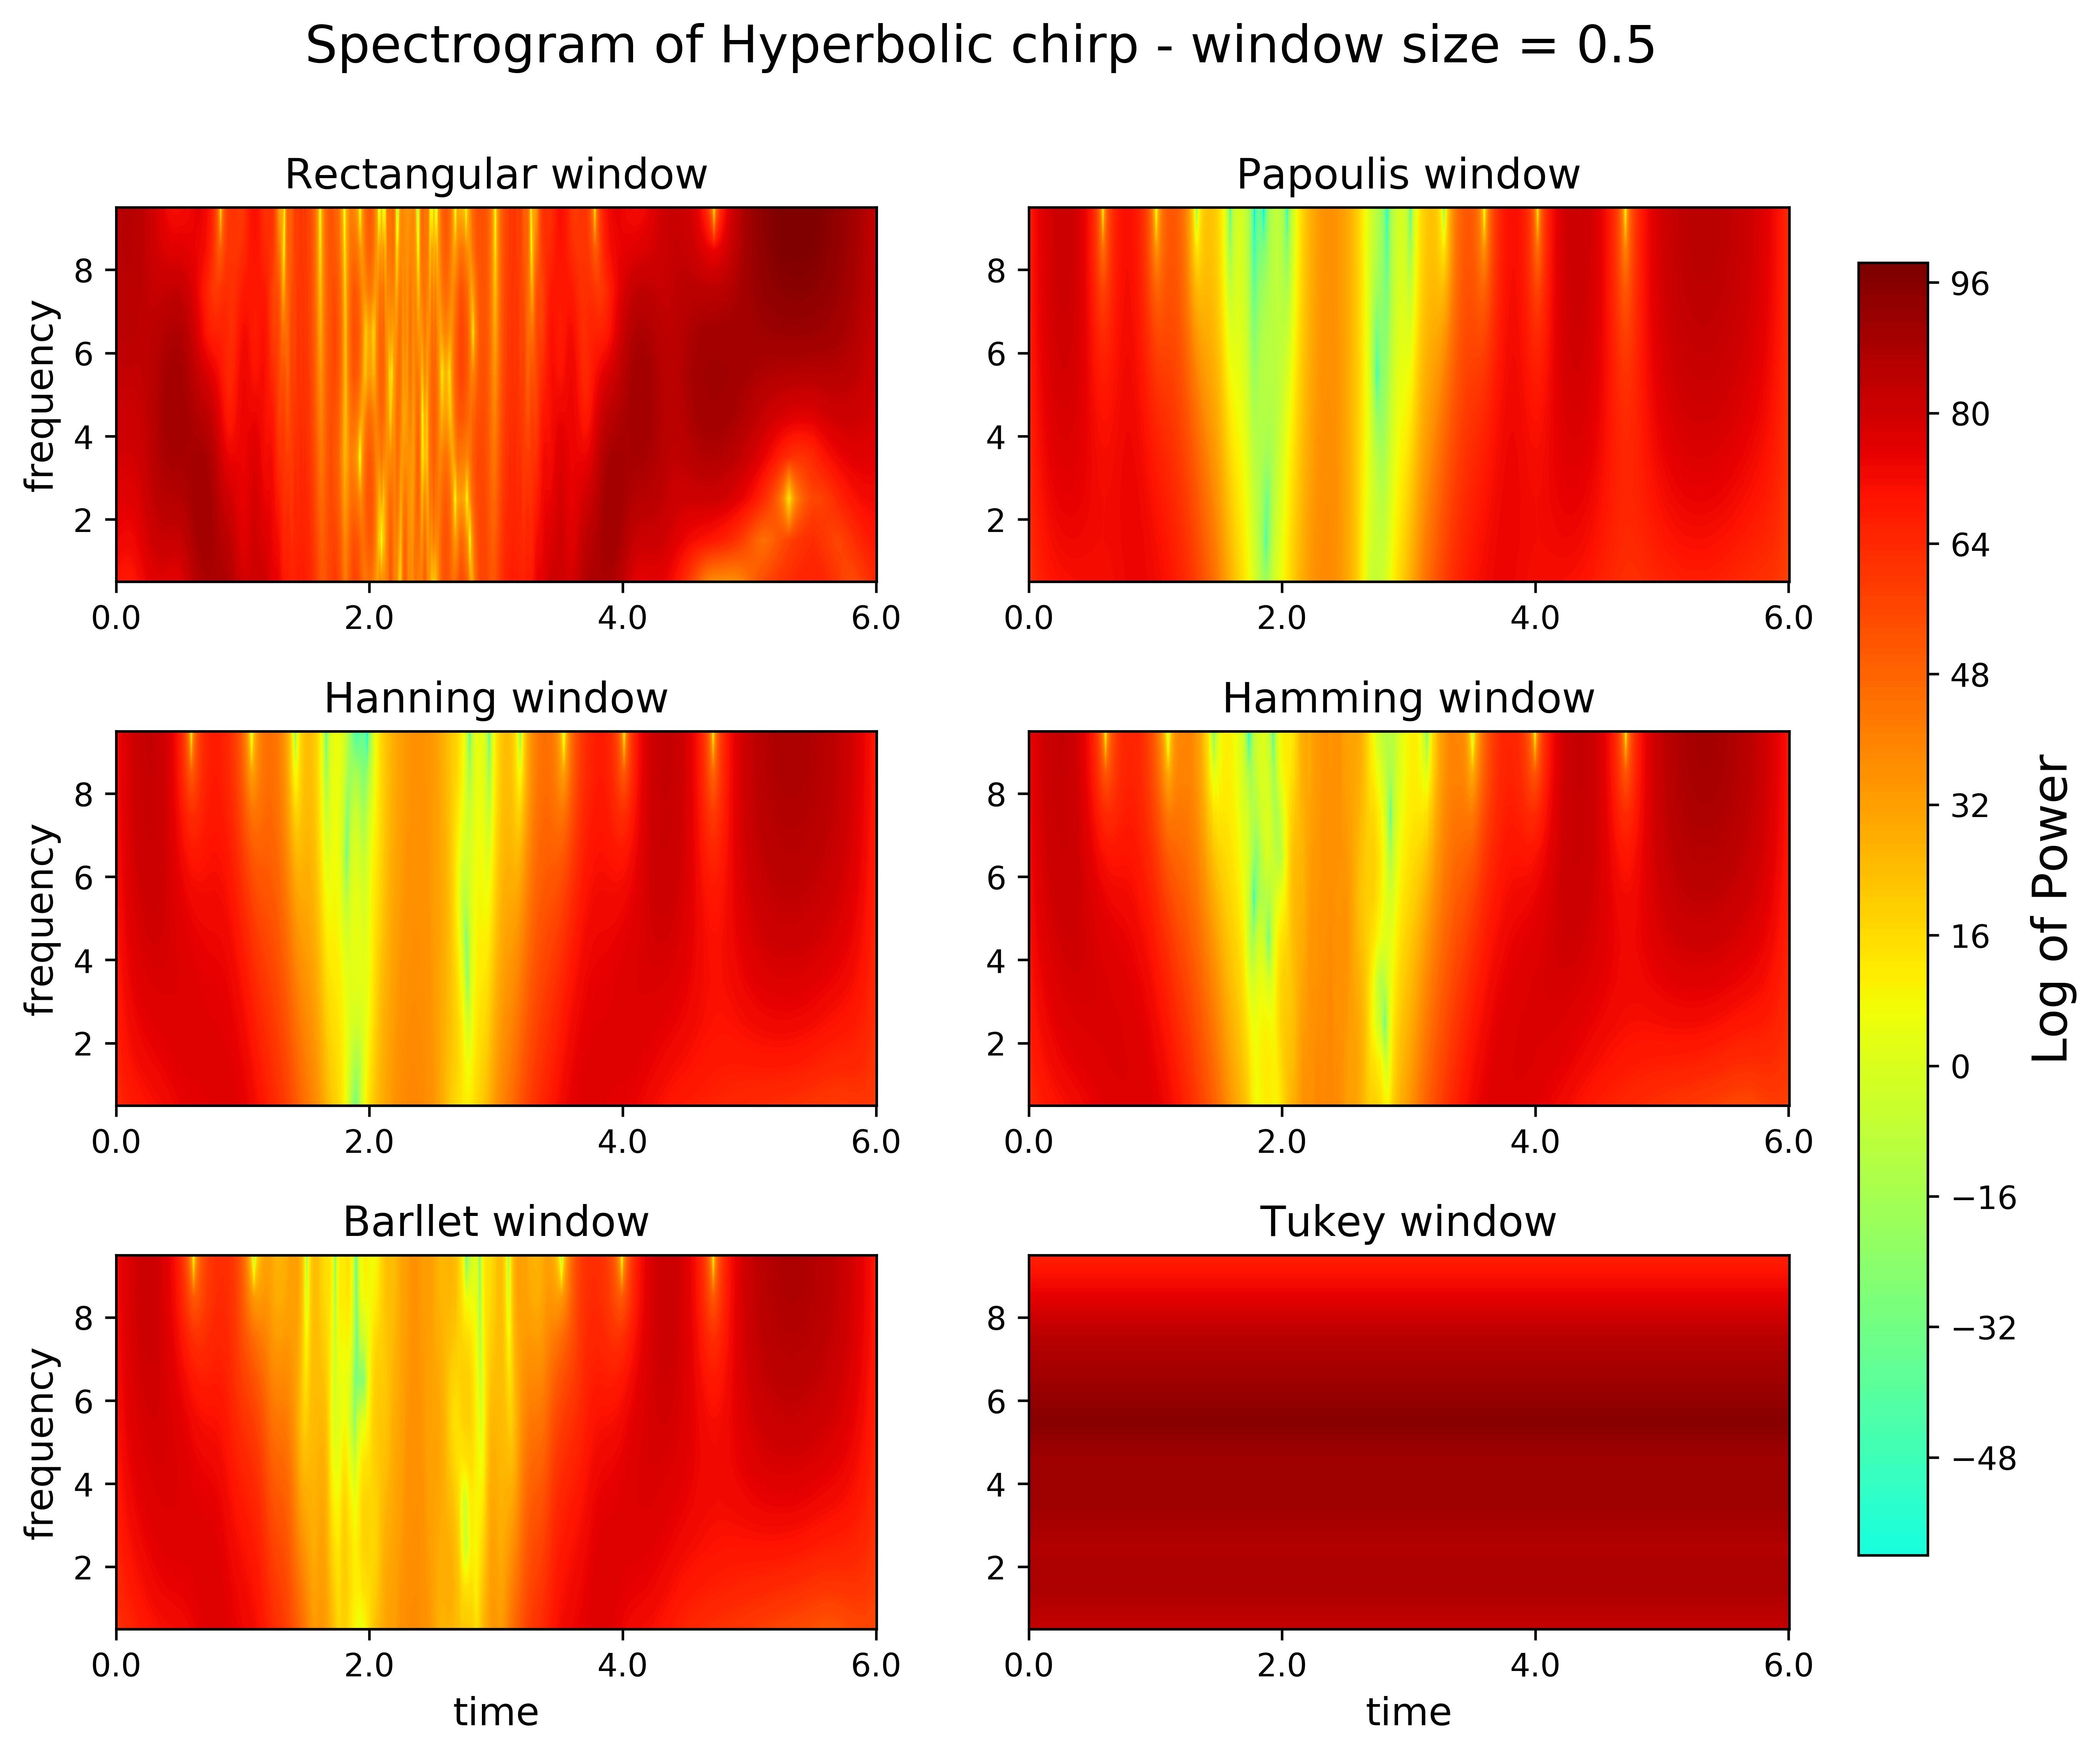
\includegraphics{../scripts/exercicio2/espectros/TEST_Hyperbolic_ws0.5.jpg}}	
	\end{center}
	\vspace{1mm}
	\label{ex1_fig1}
\end{figure}

%%%%%%%%%%%%%%%%%%%%%%%%%%%%%%%%%%%%%%%%%%%%%%%%%%%%%%%%%% 2.c

\subsection*{2.c} 
\addcontentsline{toc}{section}{\protect\numberline{} 2.c}%

Se o objetivo da análise é obter detalhes da variação das diferentes frequências do sinal ao longo do tempo, a implementação das WFT com janelas grandes é desejada, uma vez que isso oferecerá maior resolução frequencial no espectrograma. Para o chirp gaussiano, uma vez que a variação da frequência é suave e com poucos componentes, as janelas de tamanho 0.1 e 0.5 (Figuras 2.4, 2.5 e 2.6) foram equivalentes em resultado. 

Já para o chirp linear, a janela de tamanho igual a 0.1 não foi capaz de captar a variação linear (e suave) da frequência (Figura 2.7). As janelas de tamanho 0.5 conseguiram. %Em particular, na Figura 2.8 somente a janela retangular captou bem a variação da frequência. Isso pode ser explicado pela Figura 2.1, que ilustra a transformada da janela retangular como tendo a menor largura (em frequência) e, portanto, melhor resolução frequencial. %Em contrapartida, a Figura 2.4 ilustra que todas as transformadas possuem larga distribuição, ou seja, baixíssima resolução.

%Em particular, na Figura 2.8 somente a janela retangular captou bem a variação da frequência. Isso pode ser explicado pela Figura 2.1, que ilustra a transformada da janela retangular como tendo a menor largura (em frequência) e, portanto, melhor resolução frequencial. 
As Figuras 2.10 e 2.11 (chirp quadrático), quando contrastadas, também ilustram a incapacidade das janelas de tamanho igual a 0.1 de contribuir para a análise deste chirp. Na Figura 2.10, assim como na Figura 2.7, somente a janela retangular foi capaz de captar uma variação apreciável de frequência. Isso pode ser explicado pela Figura 2.1, que ilustra a transformada da janela retangular como tendo a menor largura (em frequência) e, portanto, melhor resolução frequencial. %As Figuras 2.11 e 2.12 atestam a variação quadrática da frequência do chirp analisado com o tempo.

O chirp hiperbólico foi o sinal que melhor ilustrou o \textit{trade-off} da resolução tempo $\times$ frequência por trás da definição do tamanho da janela. As Figuras 2.13 e 2.15 exibem os espectrogramas para as janelas de tamanho igual a 0.1, ou seja, de alta resolução temporal. A variação das cores (das frequências) na direção do eixo horizontal nestas figuras é bem acentuada. A WFT com estas janelas captou bem a variação temporal do sinal sem determinar bem quais frequências compõem o sinal localmente. Em contrapartida, nas Figura 2.14 e 2.16 o tamanho das janelas é 0.5, ou seja, a resolução temporal é menor. Com isso, o espectrograma exibe forte variação de cores que resulta da melhor representação de frequências, ganhando resolução vertical ao passo que perde a capacidade de descrever a variação horizontal dessas cores como antes. 

Em conjunto, as figuras desta seção atestam a capacidade da WFT de analisar conteúdos frequenciais de um sinal localmente, conferindo uma componente extra de análise: o tempo. Este componente é ausente na análise de Fourier tradicional, que possui um caráter global de análise. Com a WFT surgem parâmetros relevantes à nossa análise desde a análise de Fourier, a saber, o tamanho da função janela escolhida, diretamente relacionado ao já conhecido princípio da incerteza. Quanto maior (menor) a largura da janela, menor (maior) será a resolução temporal da ferramenta e maior (menor) será sua resolução frequencial. Por fim, outro importante parâmetro da WFT é a função janela em si, uma vez que os resultados deste exercício sugerem que, em alguns casos, algumas funções janela são mais úteis que outras em captar as diferentes frequências de um sinal.
















 %% 2o capítulo

\clearpage
%%%%%%%%%%%%%%%%%%%%%%%%%%%%%%%%%%%%%%%%%%%%%%%%%%%%%%%%%%%%%%%%%%%%%%%%%%%%%%%

\section*{\large Exercício 3}
\addcontentsline{toc}{chapter}{\protect\numberline{}\large Exercício 3}%


% EXEMPLO PARA ADICIONAR FIGURA
%\begin{figure}[ht!]
	%\caption{Série e histogramas.}
%	\vspace{0mm}	% acrescentar o espaçamento vertical apropriado entre o título e a borda superior da figura
%	\begin{center}
%		\resizebox{15cm}{!}{\includegraphics{Figuras/ex1/Exercicio1_n_64.jpg}}		
%	\end{center}
%	\vspace{-2mm}	% acrescentar o espaçamento vertical apropriado entre a borda inferior da figura e a legenda ou a fonte quando não há legenda (o valor pode ser negativo para subir)
%	\legenda{Figura 1.1: Dez sinais e seus respectivos histogramas para  asérie com $N$ = 64 do grupo noise.}	% legenda - para deixar sem legenda usar comando \legenda{} (nunca deve-se comentar o comando \legenda)
%	\label{ex1_fig1}
%	%\FONTE{}	% fonte consultada (elemento obrigatório, mesmo que seja produção do próprio autor)
%\end{figure}

%====================================================================== 3.1

\subsection*{3.1} 
\addcontentsline{toc}{section}{\protect\numberline{} 3.1}%

Resultados presentes no relatório.

\subsection*{3.2} 
\addcontentsline{toc}{section}{\protect\numberline{} 3.2}%

Relatório em preparação.





 %% 3o capítulo

\clearpage
%%%%%%%%%%%%%%%%%%%%%%%%%%%%%%%%%%%%%%%%%%%%%%%%%%%%%%%%%%%%%%%%%%%%%%%%%%%%%%%

\section*{\large Exercício 4}
\addcontentsline{toc}{chapter}{\protect\numberline{}\large Exercício 4}%

\textit{In prep.}

% EXEMPLO PARA ADICIONAR FIGURA
%\begin{figure}[ht!]
	%\caption{Série e histogramas.}
%	\vspace{0mm}	% acrescentar o espaçamento vertical apropriado entre o título e a borda superior da figura
%	\begin{center}
%		\resizebox{15cm}{!}{\includegraphics{Figuras/ex1/Exercicio1_n_64.jpg}}
%	\end{center}
%	\vspace{-2mm}	% acrescentar o espaçamento vertical apropriado entre a borda inferior da figura e a legenda ou a fonte quando não há legenda (o valor pode ser negativo para subir)
%	\legenda{Figura 1.1: Dez sinais e seus respectivos histogramas para  asérie com $N$ = 64 do grupo noise.}	% legenda - para deixar sem legenda usar comando \legenda{} (nunca deve-se comentar o comando \legenda)
%	\label{ex1_fig1}
%	%\FONTE{}	% fonte consultada (elemento obrigatório, mesmo que seja produção do próprio autor)
%\end{figure}
 %% 4o capítulo

\clearpage
%%%%%%%%%%%%%%%%%%%%%%%%%%%%%%%%%%%%%%%%%%%%%%%%%%%%%%%%%%%%%%%%%%%%%%%%%%%%%%%

\section*{\large Exercício 5}
\addcontentsline{toc}{chapter}{\protect\numberline{}\large Exercício 5}%

Verificarei a propriedade de simetria nos domínios tempo e frequência. Ela é importante pois a Análise de Fourier aproxima funções por uma soma de senos e cossenos. Portanto, funções pares necessitam apenas os termos dos cossenos, enquanto funções ímpares apenas os termos da soma associados à função seno. Isso ocorre pois, em cada caso, a outra metade dos coeficientes é igual a zero. Sendo assim, explorar simetrias pode ser importante para poupar esforço (tempo) computacional. 

\textbf{Resolução:}

Uma função geral pode ser escrita como a soma de uma função par $f_{e}$ (ou em inglês, \textit{even}) e outra ímpar $f_{o}$ (ou em inglês, \textit{odd}):

\begin{equation*}
f(x) = f_{e}(x) + f_{o}(x).
\end{equation*}

Uma função par é tal que $f(x) =  f(-x)$, ou seja, ela é simétrica com relação ao eixo das ordenadas. Uma função ímpar é tal que $f(x) =  -f(-x)$, ou seja, ela é antissimétrica. Além disso, tem-se que $\int_{-\infty}^{\infty}f_{e}(x)dx = 2 \int_{0}^{\infty}f_{e}(x)dx$, ao passo que $\int_{-\infty}^{\infty}f_{o}(x)dx = 0$. Por último, a multiplicação de funções pares por funções ímpares é tal que: $f_{e} \times g_{e} = h_{e}$, $f_{o} \times g_{o} = h_{e}$, e $f_{e} \times g_{o} = h_{o}$.

A partir destas propriedades de uma função geral, e da propriedade de linearidade da Transformada de Fourier (verificadda no Exercício 2), podemos escrever a Eq. 1 como:

\begin{align*}
\hat{f}(\xi) &= \int_{-\infty}^{+\infty} f(t) e^{-\imath \xi t}d t \\
 &= \int_{-\infty}^{+\infty} f_{e}(x) e^{-\imath \xi t}d t  + \int_{-\infty}^{+\infty}  f_{o}(x) e^{-\imath \xi t}d t \\[10pt]
 &= \int_{-\infty}^{+\infty} f_{e}(x) \cos(\xi t)d t  - \imath \cancelto{0}{\int_{-\infty}^{+\infty}  f_{e}(x) \sin(\xi t)d t} + \\[10pt]
 & \quad \cancelto{0}{\int_{-\infty}^{+\infty} f_{o}(x) \cos(\xi t)d t} - \imath \int_{-\infty}^{+\infty}  f_{o}(x) \sin(\xi t)d t \\[10pt]
  &= 2 \int_{0}^{+\infty} f_{e}(x) \cos(\xi t)d t - 2 \imath \int_{0}^{+\infty}  f_{o}(x) \sin(\xi t)d t.
\end{align*}

Similarmente, podemos escrever para uma função complexa $f(x) = f_{re}(x) + \imath f_{im}(x)$:

\begin{align*}
\hat{f}(\xi) &= \int_{-\infty}^{+\infty} f(t) e^{-\imath \xi t}d t \\[10pt]
 &= \int_{-\infty}^{+\infty} f_{re}(x) e^{-\imath \xi t}d t  + \imath \int_{-\infty}^{+\infty}  f_{im}(x) e^{-\imath \xi t}d t \\[10pt]
 &= \int_{-\infty}^{+\infty} f_{re}(x) \cos(\xi t)d t  - \imath\int_{-\infty}^{+\infty}  f_{re}(x) \sin(\xi t)d t + \\[10pt]
 & \quad \imath \int_{-\infty}^{+\infty} f_{im}(x) \cos(\xi t)d t + \imath \int_{-\infty}^{+\infty}  f_{im}(x) \sin(\xi t)d t.
\end{align*}

Dessa maneira, a depender da natureza da função $f(x)$, o produto de funções em cada uma das quatro integrais somadas acima resultará numa função par ou ímpar, de modo que somente uma destas integrais será diferente de zero. A tabela abaixo resume os possíveis resultados.

\begin{table*}[ht!]
\legenda{Tabela 5.1: Propriedades de simetria nos domínios tempo e frequência.\vspace{.9mm}}
\centering
\raa{1.3}
\begin{tabular}{@{}l l l l@{}}
\toprule
%\hline
$f(x)$ é & Integral restante & O resultado de $\hat{f}(\xi)$ é \\
\cmidrule{1-3}
real e par & 1$^{\text{a}}$  & real e par \\
real e ímpar & 2$^{\text{a}}$ & imaginária e ímpar \\
imaginária e par & 3$^{\text{a}}$ & imaginária e par \\
imaginária e ímpar & 4$^{\text{a}}$ & real e ímpar \\
\bottomrule
\end{tabular}
\label{tab:1}
\end{table*}

As Figuras a seguir ilustram as propriedades da Tabela 5.1. 

A Figura 5.1 exibe as funções trigonométricas reais, uma par $f_{1}(t)$ (gráfico do topo à esquerda com a função cosseno) e outra ímpar  $f_{2}(t)$ (gráfico de baixo à esquerda com a função seno), ambas de período igual a 10. Suas respectivas transformadas à direita, $\hat{f}_{1}(t)$ (real e par) e  $\hat{f}_{2}(t)$ (imaginária e ímpar), atestam as propriedades da Tabela 5.1. A Figura 5.2 complementa as informações da tabela exibindo as mesmas funções porém  puramente imaginárias (multiplicadas pelo número imaginário $\imath = \sqrt{-1}$). Nesse caso, $\hat{f}_{1}(t)$ é imaginária e par enquanto $\hat{f}_{2}(t)$ é real e ímpar. As Figuras 5.3 e 5.4 refazem a análise das Figuras 5.1 e 5.2, respectivamente, para duas novas funções: uma polinomial par $f_{1}(t) = t^{2}$, e outra polinomial ímpar $f_{2}(t) = t^{3}$. Suas respectivas transformadas fomentam a análise implementada durante a resolução deste exercício, pois também ilustram as propriedades de simetria da transformada de Fourier presentes na Tabela 5.1.

\begin{figure}[ht!]
	\legenda{Figura 5.1: Transformada de Fourier de duas funções trigonométricas reais, uma par e outra ímpar. A transformada da primeira é real e par, já da segunda é imaginária e ímpar.}
	\vspace{-1mm}	% acrescentar o espaçamento vertical apropriado entre o título e a borda superior da figura
	\begin{center}
		\resizebox{\textwidth}{!}{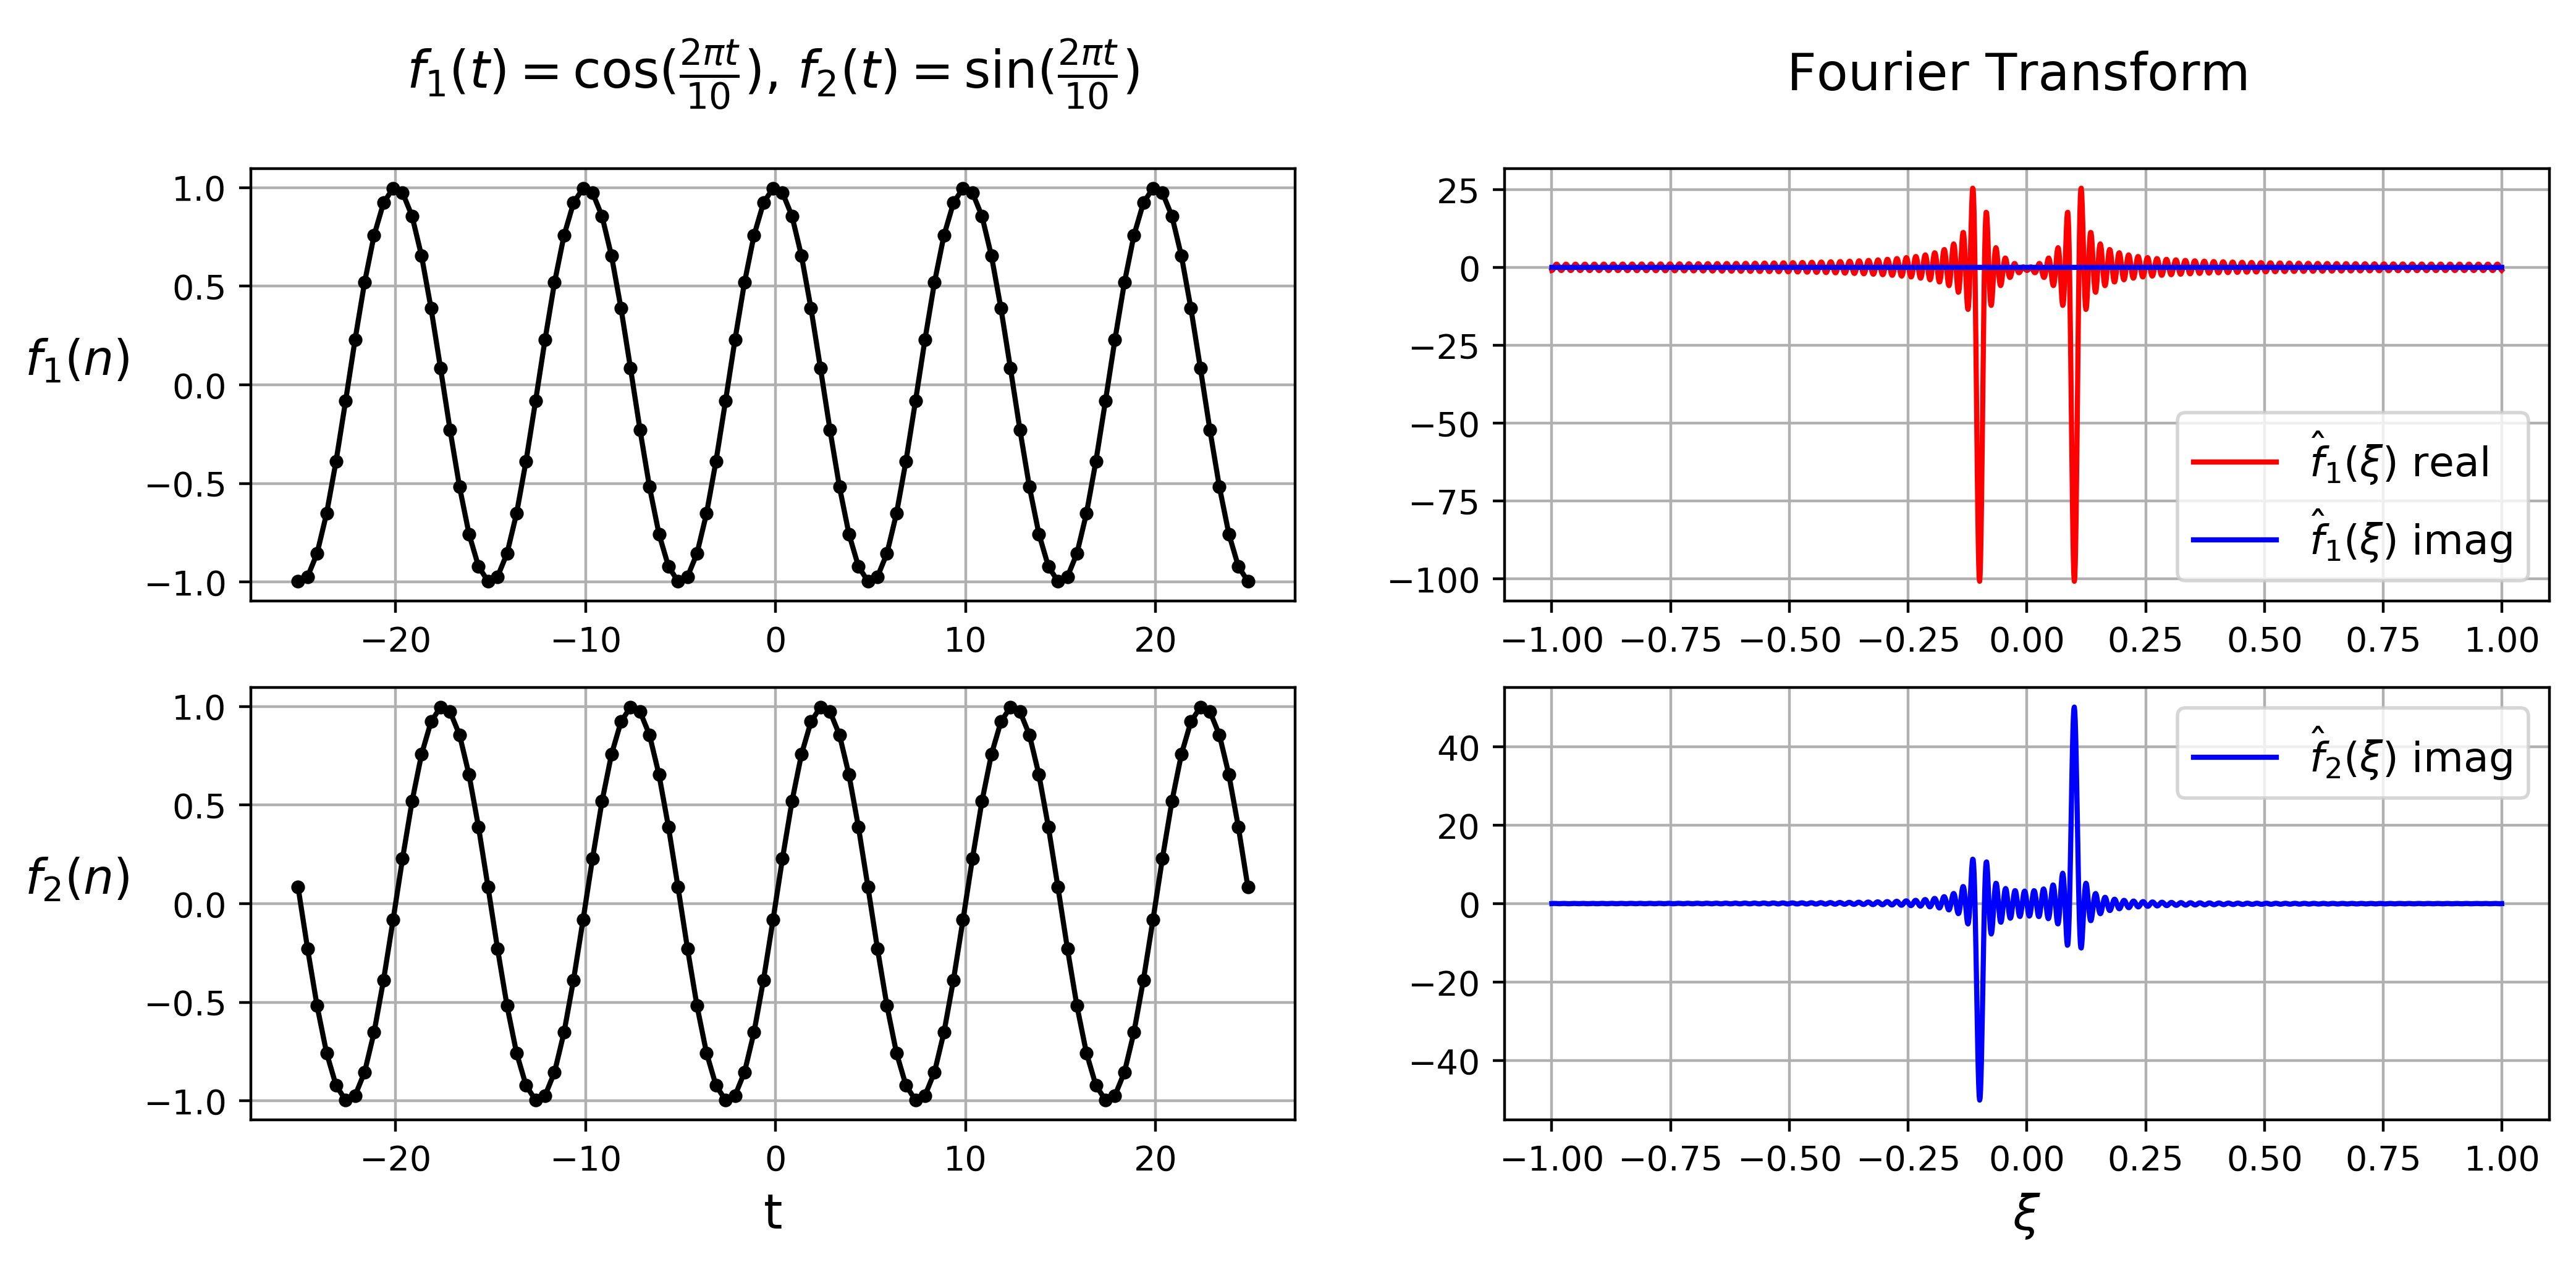
\includegraphics{../scripts/exercicio5/ft_symetries_real_trig.jpg}}	
	\end{center}
	\vspace{-2mm}	% acrescentar o espaçamento vertical apropriado entre a borda inferior da figura e a legenda ou a fonte quando não há legenda (o valor pode ser negativo para subir)
	%\legenda{Figura 1.1: Dez sinais e seus respectivos histogramas para  asérie com $N$ = 64 do grupo noise.}	% legenda - para deixar sem legenda usar comando \legenda{} (nunca deve-se comentar o comando \legenda)
	\label{ex1_fig1}
	%\FONTE{}	% fonte consultada (elemento obrigatório, mesmo que seja produção do próprio autor)
\end{figure}

\begin{figure}[ht!]
	\legenda{Figura 5.2: Transformada de Fourier de duas funções trigonométricas imaginárias, uma par e outra ímpar. A transformada da primeira é imaginária e par, já da segunda é real e ímpar.}
	\vspace{-1mm}	% acrescentar o espaçamento vertical apropriado entre o título e a borda superior da figura
	\begin{center}
		\resizebox{\textwidth}{!}{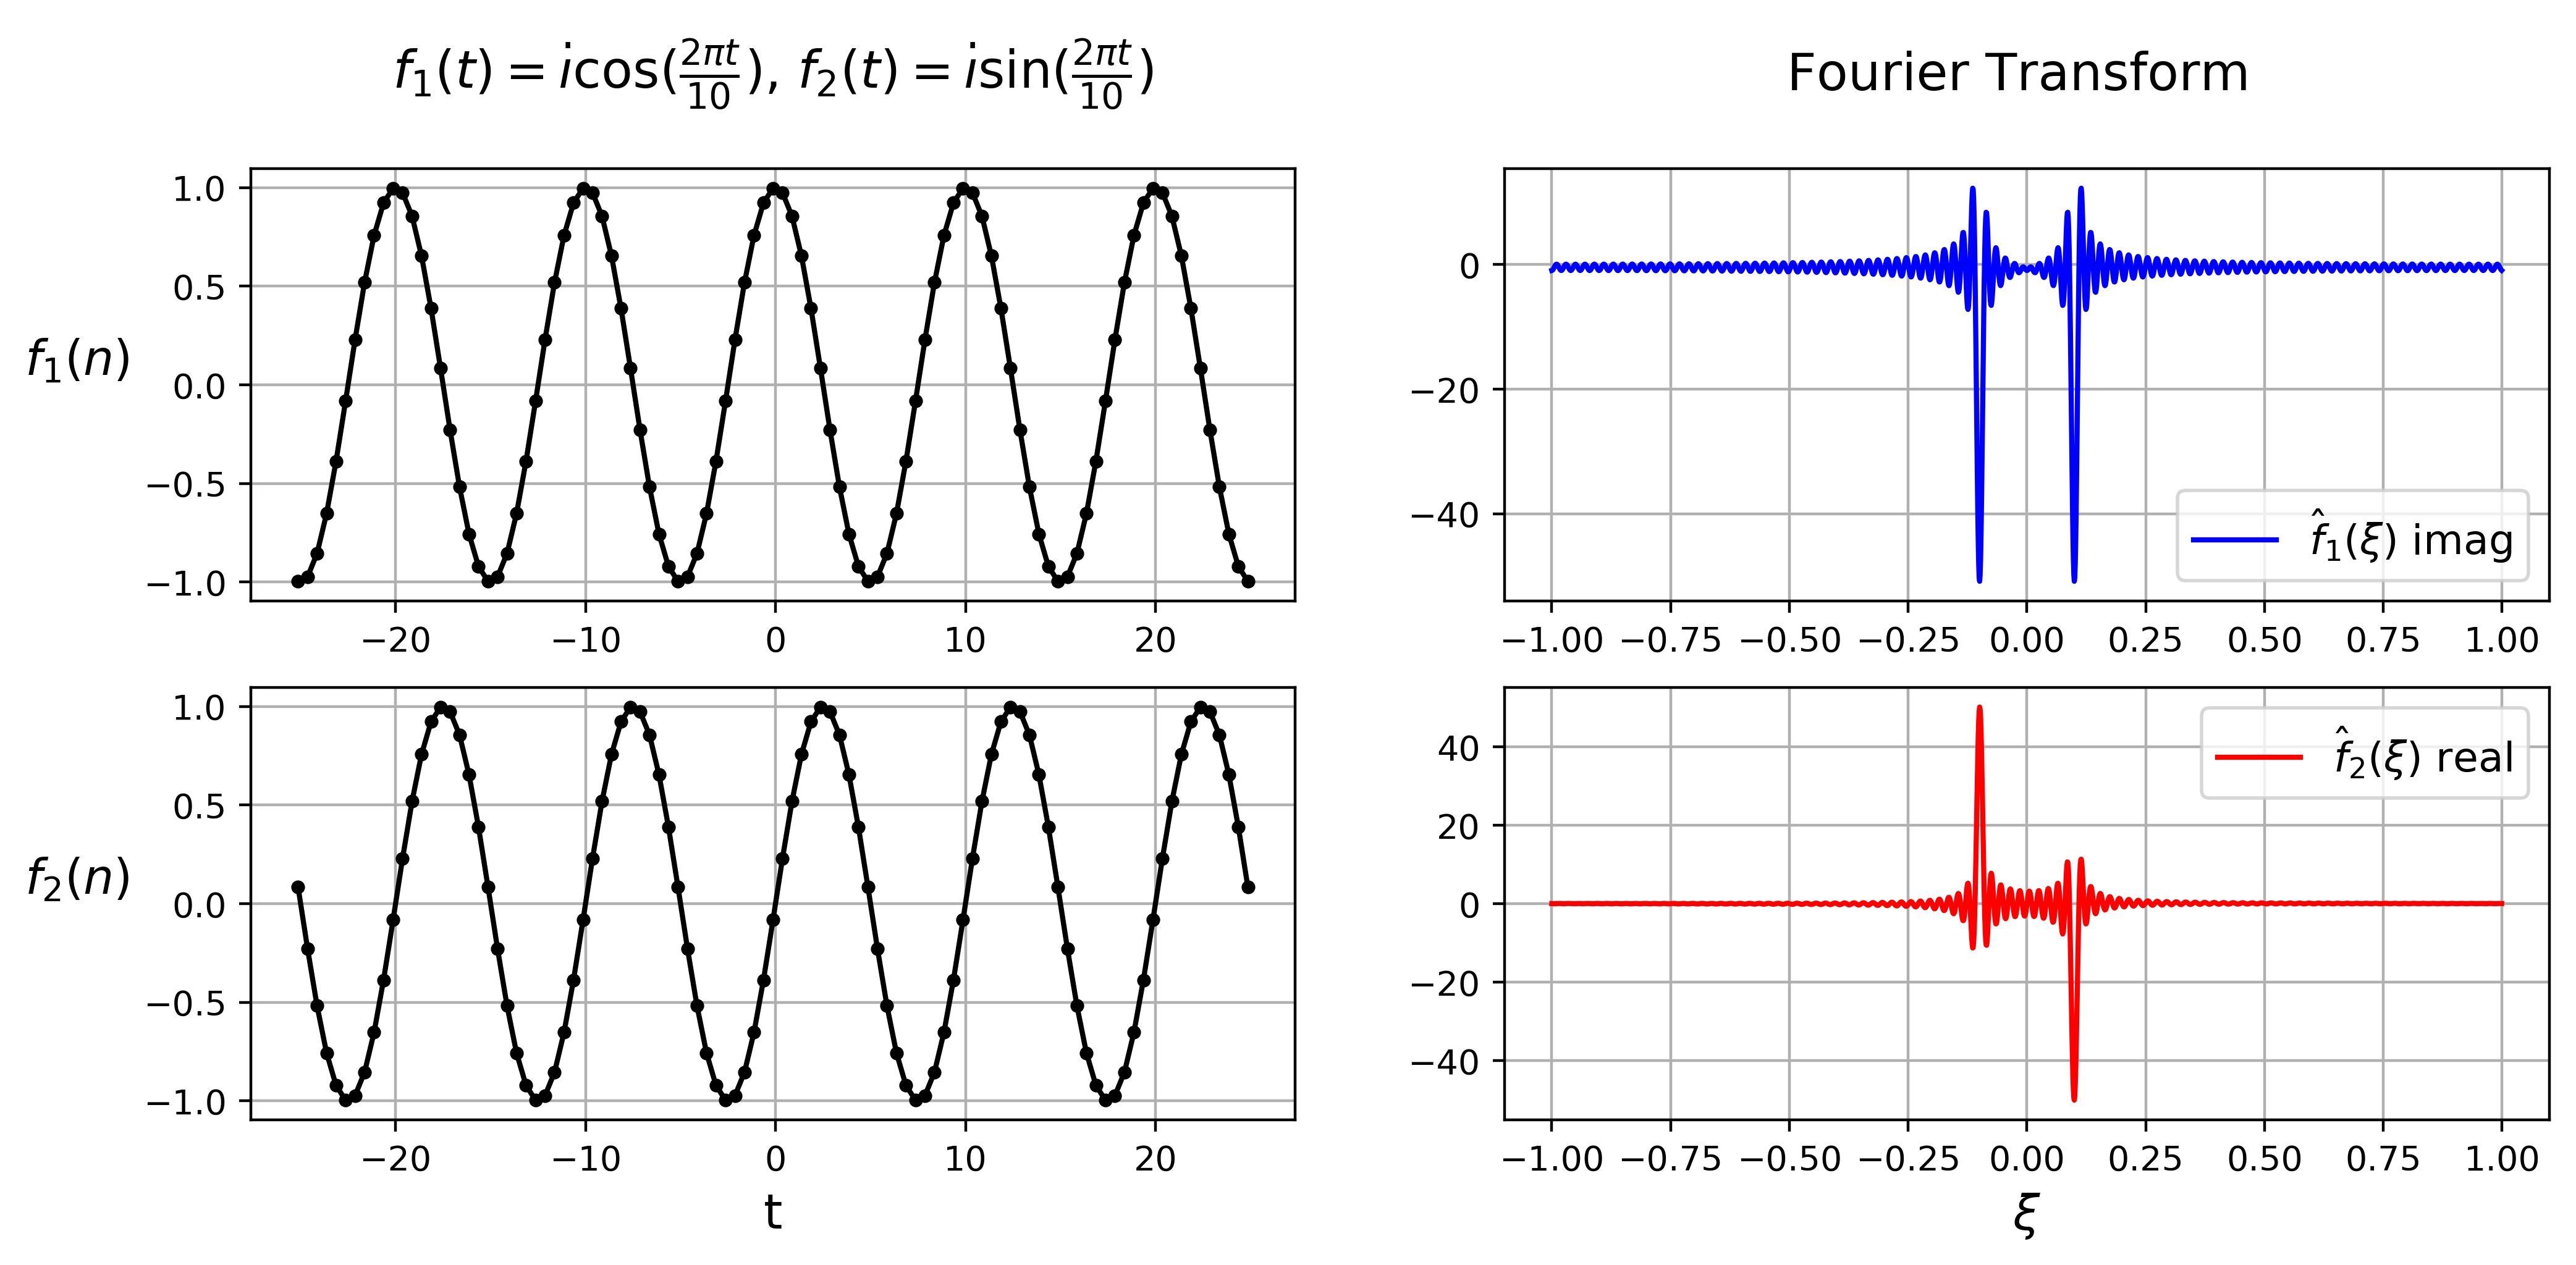
\includegraphics{../scripts/exercicio5/ft_symetries_imag_trig.jpg}}	
	\end{center}
	\vspace{-2mm}	% acrescentar o espaçamento vertical apropriado entre a borda inferior da figura e a legenda ou a fonte quando não há legenda (o valor pode ser negativo para subir)
	%\legenda{Figura 1.1: Dez sinais e seus respectivos histogramas para  asérie com $N$ = 64 do grupo noise.}	% legenda - para deixar sem legenda usar comando \legenda{} (nunca deve-se comentar o comando \legenda)
	\label{ex1_fig1}
	%\FONTE{}	% fonte consultada (elemento obrigatório, mesmo que seja produção do próprio autor)
\end{figure}

%============================ polys

\begin{figure}[ht!]
	\legenda{Figura 5.3: Transformada de Fourier de duas funções polinomiais reais, uma par e outra ímpar. A transformada da primeira é real e par, já da segunda é imaginária e ímpar.}
	\vspace{-1mm}	% acrescentar o espaçamento vertical apropriado entre o título e a borda superior da figura
	\begin{center}
		\resizebox{\textwidth}{!}{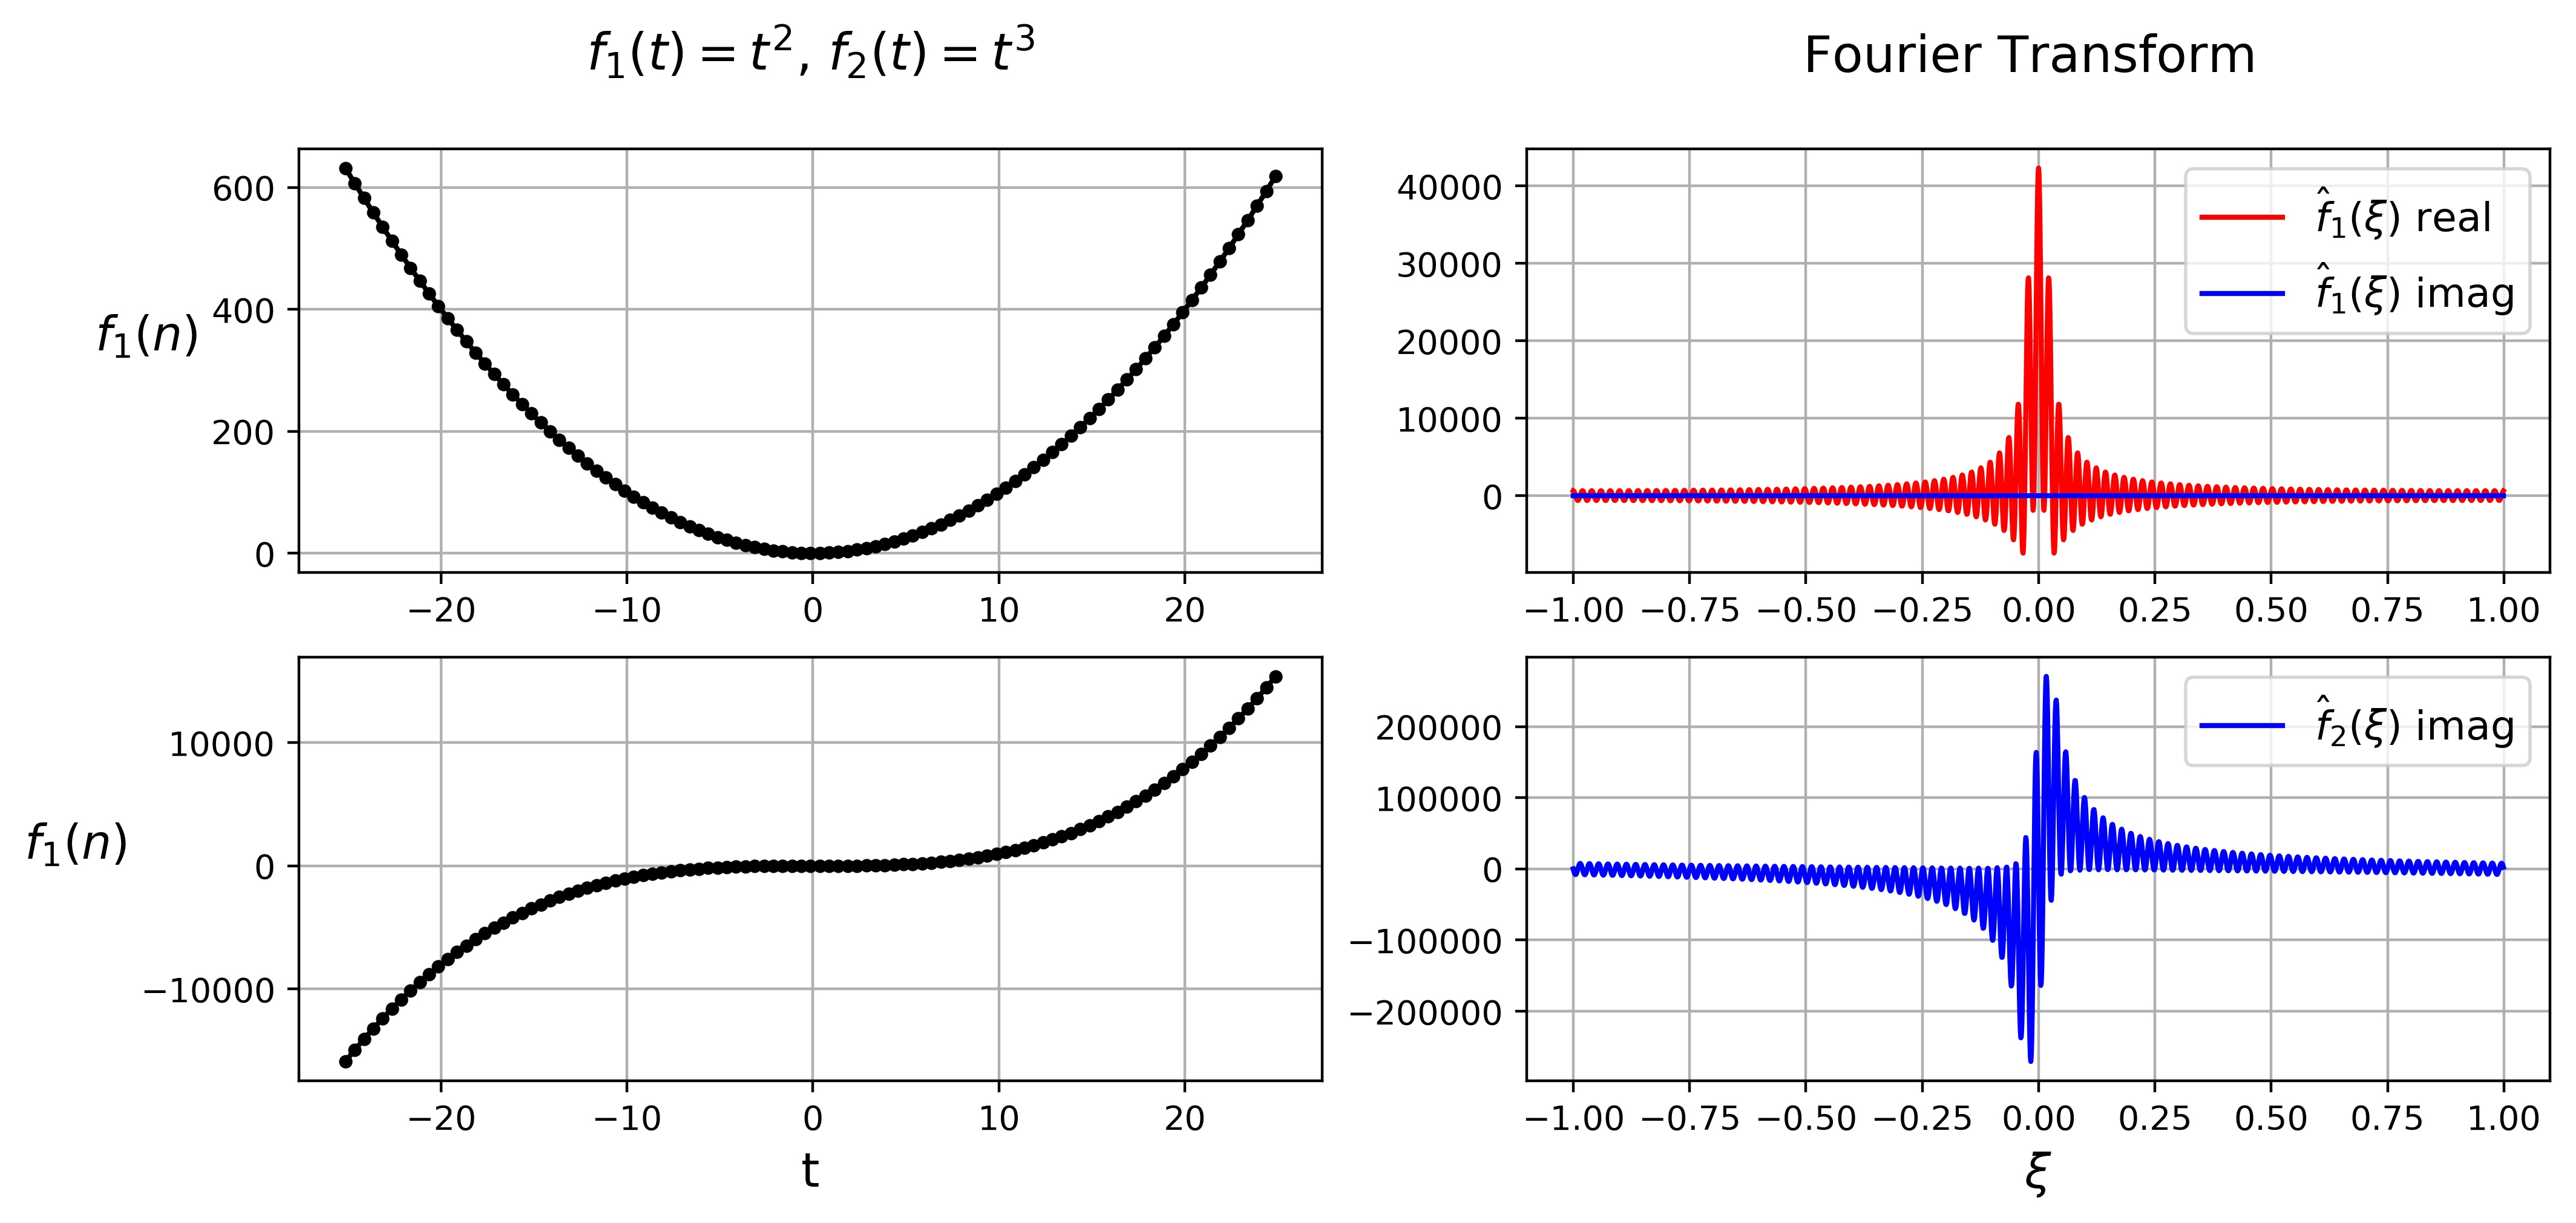
\includegraphics{../scripts/exercicio5/ft_symetries_real_poly.jpg}}	
	\end{center}
	\vspace{-2mm}	% acrescentar o espaçamento vertical apropriado entre a borda inferior da figura e a legenda ou a fonte quando não há legenda (o valor pode ser negativo para subir)
	%\legenda{Figura 1.1: Dez sinais e seus respectivos histogramas para  asérie com $N$ = 64 do grupo noise.}	% legenda - para deixar sem legenda usar comando \legenda{} (nunca deve-se comentar o comando \legenda)
	\label{ex1_fig1}
	%\FONTE{}	% fonte consultada (elemento obrigatório, mesmo que seja produção do próprio autor)
\end{figure}

\begin{figure}[ht!]
	\legenda{Figura 5.4: Transformada de Fourier de duas funções polinomiais imaginárias, uma par e outra ímpar. A transformada da primeira é imaginária e par, já da segunda é real e ímpar.}
	\vspace{-1mm}	% acrescentar o espaçamento vertical apropriado entre o título e a borda superior da figura
	\begin{center}
		\resizebox{\textwidth}{!}{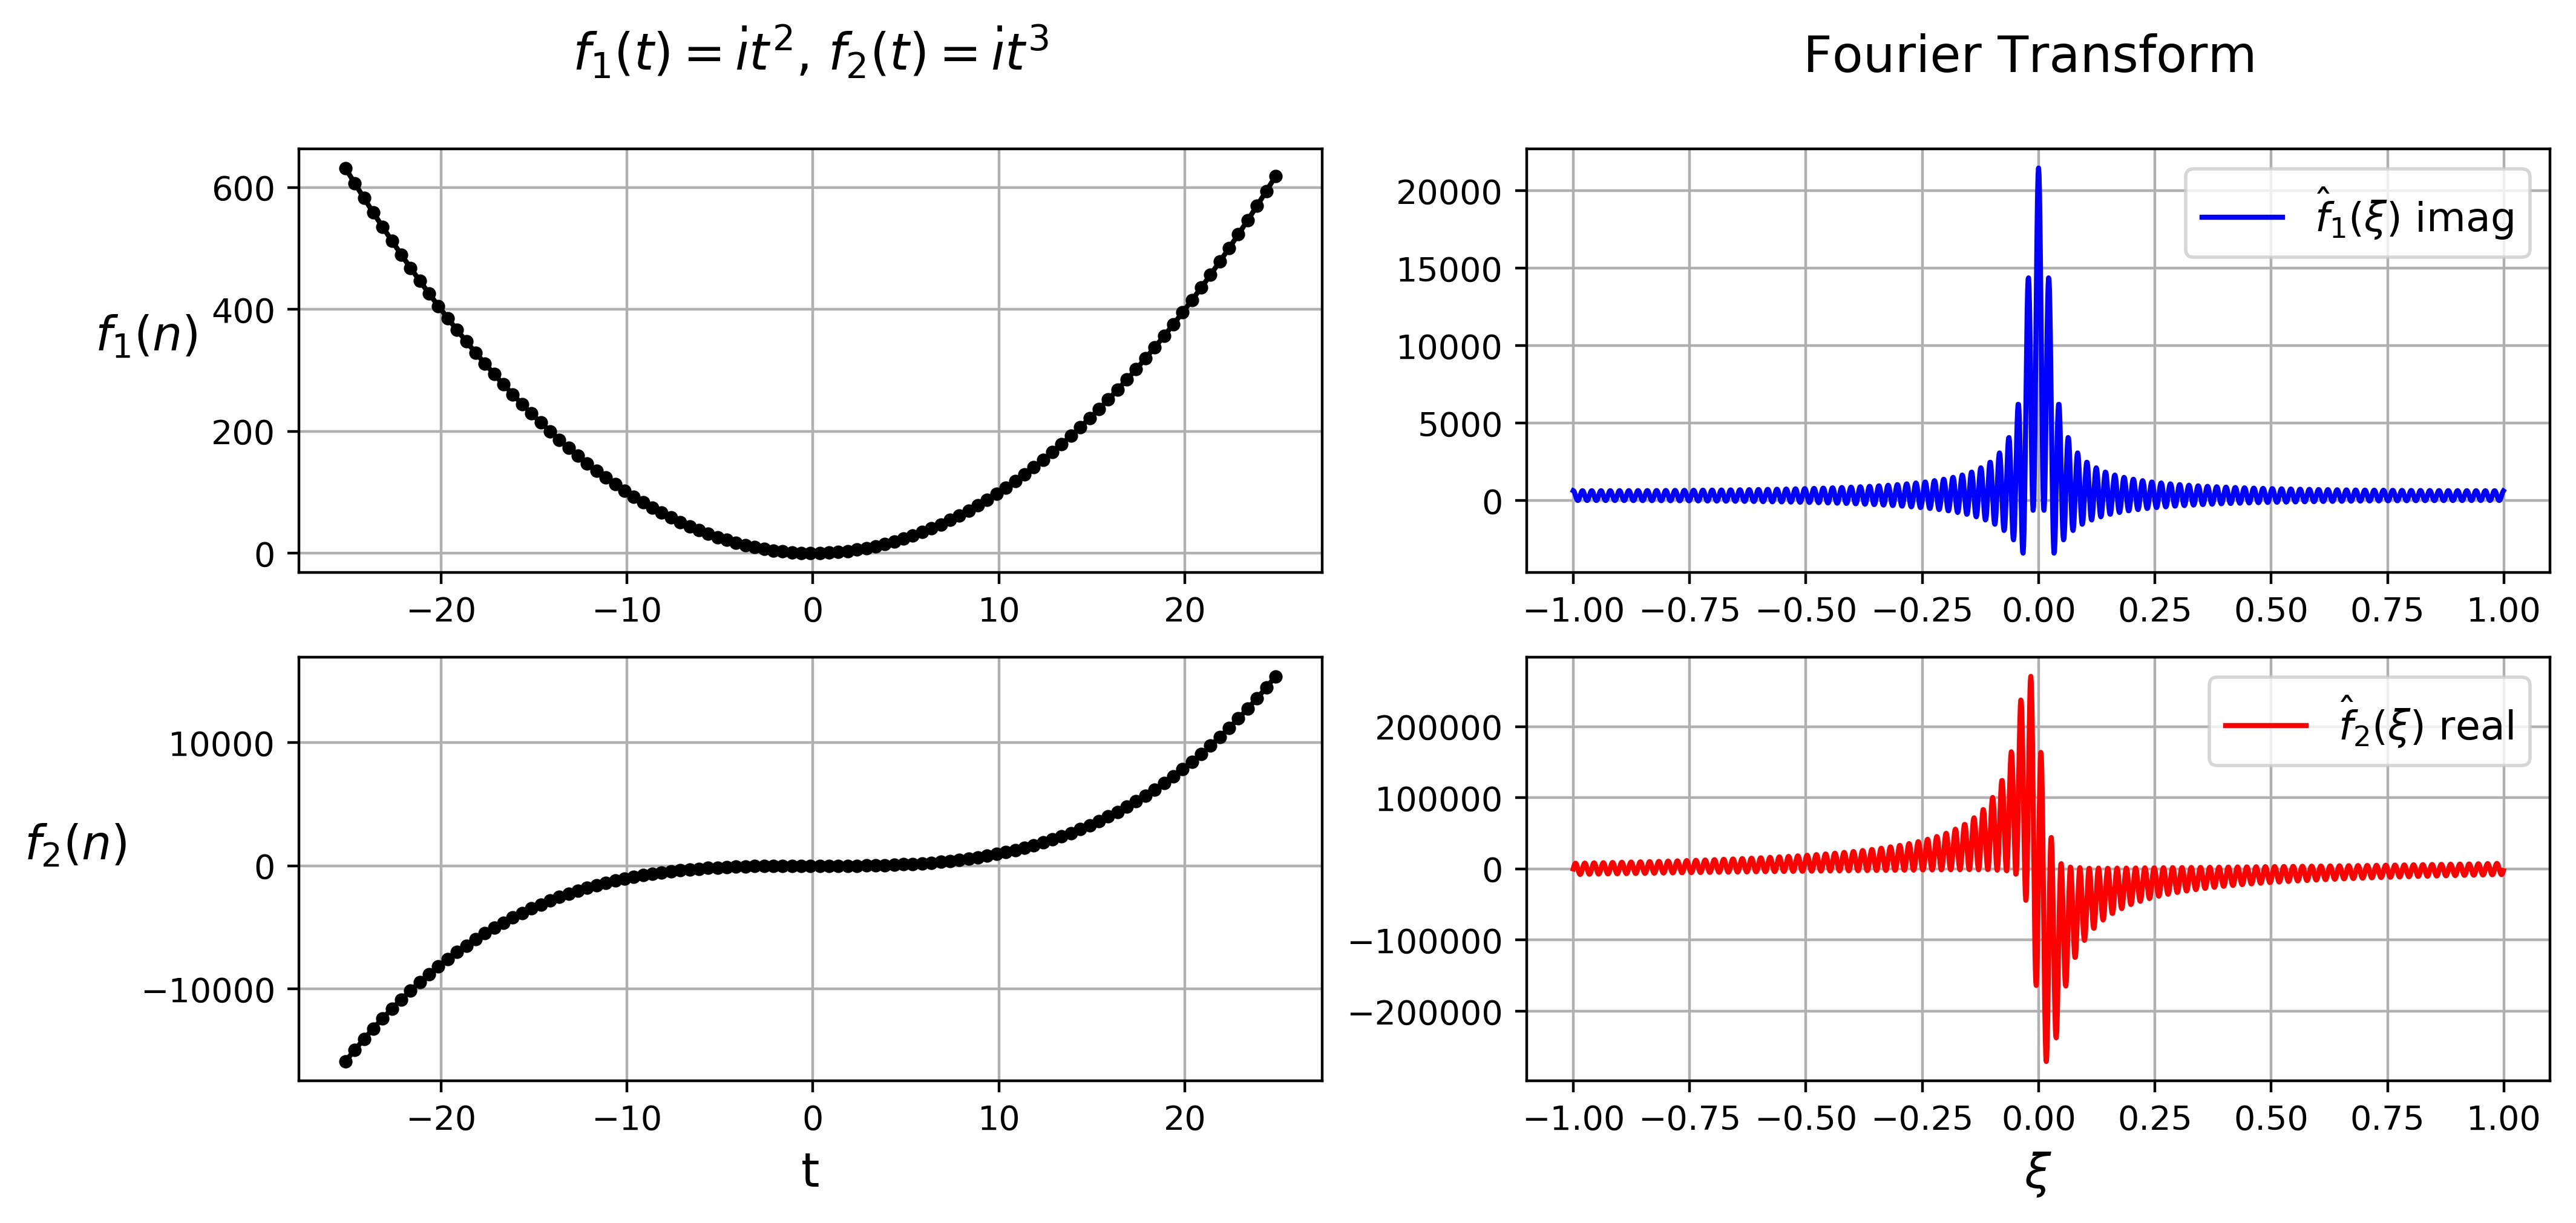
\includegraphics{../scripts/exercicio5/ft_symetries_imag_poly.jpg}}	
	\end{center}
	\vspace{-2mm}	% acrescentar o espaçamento vertical apropriado entre a borda inferior da figura e a legenda ou a fonte quando não há legenda (o valor pode ser negativo para subir)
	%\legenda{Figura 1.1: Dez sinais e seus respectivos histogramas para  asérie com $N$ = 64 do grupo noise.}	% legenda - para deixar sem legenda usar comando \legenda{} (nunca deve-se comentar o comando \legenda)
	\label{ex1_fig1}
	%\FONTE{}	% fonte consultada (elemento obrigatório, mesmo que seja produção do próprio autor)
\end{figure}
% EXEMPLO PARA ADICIONAR FIGURA
%\begin{figure}[ht!]
	%\caption{Série e histogramas.}
%	\vspace{0mm}	% acrescentar o espaçamento vertical apropriado entre o título e a borda superior da figura
%	\begin{center}
%		\resizebox{15cm}{!}{\includegraphics{Figuras/ex1/Exercicio1_n_64.jpg}}		
%	\end{center}
%	\vspace{-2mm}	% acrescentar o espaçamento vertical apropriado entre a borda inferior da figura e a legenda ou a fonte quando não há legenda (o valor pode ser negativo para subir)
%	\legenda{Figura 1.1: Dez sinais e seus respectivos histogramas para  asérie com $N$ = 64 do grupo noise.}	% legenda - para deixar sem legenda usar comando \legenda{} (nunca deve-se comentar o comando \legenda)
%	\label{ex1_fig1}
%	%\FONTE{}	% fonte consultada (elemento obrigatório, mesmo que seja produção do próprio autor)
%\end{figure}
 %% 1o capítulo, começo do texto

\clearpage
%%%%%%%%%%%%%%%%%%%%%%%%%%%%%%%%%%%%%%%%%%%%%%%%%%%%%%%%%%%%%%%%%%%%%%%%%%%%%%%

\section*{\large Exercício 6}
\addcontentsline{toc}{chapter}{\protect\numberline{}\large Exercício 6}%

\textit{In prep.}

%\textbf{Resolução:}

%\begin{equation*}
%F_{8} =
%\begin{bmatrix}
%a & b & c & d & a & b & c & d \\
%d & e & f & d & a & b & c & d \\
%g & h & i & d & a & b & c & d \\
%a & b & c & d & a & b & c & d \\
%d & e & f & d & a & b & c & d \\
%g & h & i & d & a & b & c & d \\
%a & b & c & d & a & b & c & d \\
%d & e & f & d & a & b & c & d
%\end{bmatrix}
%\end{equation*}

% EXEMPLO PARA ADICIONAR FIGURA
%\begin{figure}[ht!]
	%\caption{Série e histogramas.}
%	\vspace{0mm}	% acrescentar o espaçamento vertical apropriado entre o título e a borda superior da figura
%	\begin{center}
%		\resizebox{15cm}{!}{\includegraphics{Figuras/ex1/Exercicio1_n_64.jpg}}
%	\end{center}
%	\vspace{-2mm}	% acrescentar o espaçamento vertical apropriado entre a borda inferior da figura e a legenda ou a fonte quando não há legenda (o valor pode ser negativo para subir)
%	\legenda{Figura 1.1: Dez sinais e seus respectivos histogramas para  asérie com $N$ = 64 do grupo noise.}	% legenda - para deixar sem legenda usar comando \legenda{} (nunca deve-se comentar o comando \legenda)
%	\label{ex1_fig1}
%	%\FONTE{}	% fonte consultada (elemento obrigatório, mesmo que seja produção do próprio autor)
%\end{figure}
 %% 2o capítulo

\clearpage
%%%%%%%%%%%%%%%%%%%%%%%%%%%%%%%%%%%%%%%%%%%%%%%%%%%%%%%%%%%%%%%%%%%%%%%%%%%%%%%

\section*{\large Exercício 7}
\addcontentsline{toc}{chapter}{\protect\numberline{}\large Exercício 7}%

Mostrarei, por indução, a complexidade $\mathcal{O}(n\log_{2}{}n)$ de um algoritmo.

\textbf{Resolução:}

O algoritmo FFT funciona dividindo a soma discreta da DFT de um input de tamanho $n=2^{k}$ em duas somas: uma em $n/2$ termos pares e outra em $n/2$ termos ímpares. Esse procedimento pode ser implementado recursivamente, de modo que a cada passo de divisão pela metade teremos de computar $n$ termos através de somas distintas. 

Um algoritmo com essa característica, que precisa realizar $n$ operações antes, durante e após dividi-las em duas metades, pode ser expresso pela seguinte equação de recorrência ($T_{n}$ denota o valor de uma função $T(n)$ de complexidade de tempo em função do tamanho do input $n$)

\begin{equation*}
 \left\{ \begin{array}{rl} 
T_{n} = 2 T_{\frac{n}{2}} + n,  & n \geq 2  \\
T_{1} = 0.  & 
\end{array}\right.
\end{equation*}

Reescrevendo $T_{n}$:

\begin{align*}
T_{n} = T_{2^{k}} &= 2 T_{2^{k-1}} + 2^{k} \\[10pt]
 \frac{T_{2^{k}}}{2^{k}} &= \frac{2 T_{2^{k-1}} + 2^{k}}{2^{k}} = \frac{2 T_{2^{k-1}}}{2^{k}} + \frac{2^{k}}{2^{k}} \\[10pt]
 \frac{T_{2^{k}}}{2^{k}} &= \frac{T_{2^{k-1}}}{2^{k-1}} + 1 \\[10pt]
 \frac{T_{2^{k}}}{2^{k}} &= \frac{T_{2^{k-2}}}{2^{k-2}} + 1 + 1 \\
 &\vdots \\
 \frac{T_{2^{k}}}{2^{k}} &= \frac{T_{2^{0}}}{2^{0}} + \ldots + 1 + 1 \\[10pt]
 \frac{T_{2^{k}}}{2^{k}} &= 0 + \ldots + 1 + 1 \\[10pt]
 \frac{T_{2^{k}}}{2^{k}} &= k.
\end{align*}

Lembrando que $n=2^{k}$, temos que $k=\log_{2}n$, e a última relação pode ser reescrita:

\begin{align*}
 \frac{T_{2^{k}}}{2^{k}} = \frac{T_{n}}{n} &= \log_{2} n \\
 T_{n} &= n \log_{2} n \tag*{(Q.E.D.)}
\end{align*}

% EXEMPLO PARA ADICIONAR FIGURA
%\begin{figure}[ht!]
	%\caption{Série e histogramas.}
%	\vspace{0mm}	% acrescentar o espaçamento vertical apropriado entre o título e a borda superior da figura
%	\begin{center}
%		\resizebox{15cm}{!}{\includegraphics{Figuras/ex1/Exercicio1_n_64.jpg}}		
%	\end{center}
%	\vspace{-2mm}	% acrescentar o espaçamento vertical apropriado entre a borda inferior da figura e a legenda ou a fonte quando não há legenda (o valor pode ser negativo para subir)
%	\legenda{Figura 1.1: Dez sinais e seus respectivos histogramas para  asérie com $N$ = 64 do grupo noise.}	% legenda - para deixar sem legenda usar comando \legenda{} (nunca deve-se comentar o comando \legenda)
%	\label{ex1_fig1}
%	%\FONTE{}	% fonte consultada (elemento obrigatório, mesmo que seja produção do próprio autor)
%\end{figure}
 %% 3o capítulo

\clearpage
%%%%%%%%%%%%%%%%%%%%%%%%%%%%%%%%%%%%%%%%%%%%%%%%%%%%%%%%%%%%%%%%%%%%%%%%%%%%%%%

\section*{\large Exercício 8}
\addcontentsline{toc}{chapter}{\protect\numberline{}\large Exercício 8}%

\textit{In prep.}

% EXEMPLO PARA ADICIONAR FIGURA
%\begin{figure}[ht!]
	%\caption{Série e histogramas.}
%	\vspace{0mm}	% acrescentar o espaçamento vertical apropriado entre o título e a borda superior da figura
%	\begin{center}
%		\resizebox{15cm}{!}{\includegraphics{Figuras/ex1/Exercicio1_n_64.jpg}}		
%	\end{center}
%	\vspace{-2mm}	% acrescentar o espaçamento vertical apropriado entre a borda inferior da figura e a legenda ou a fonte quando não há legenda (o valor pode ser negativo para subir)
%	\legenda{Figura 1.1: Dez sinais e seus respectivos histogramas para  asérie com $N$ = 64 do grupo noise.}	% legenda - para deixar sem legenda usar comando \legenda{} (nunca deve-se comentar o comando \legenda)
%	\label{ex1_fig1}
%	%\FONTE{}	% fonte consultada (elemento obrigatório, mesmo que seja produção do próprio autor)
%\end{figure}
 %% 4o capítulo

\clearpage
%%%%%%%%%%%%%%%%%%%%%%%%%%%%%%%%%%%%%%%%%%%%%%%%%%%%%%%%%%%%%%%%%%%%%%%%%%%%%%%

\section*{\large Exercício 9}
\addcontentsline{toc}{chapter}{\protect\numberline{}\large Exercício 9}%

\textit{In prep.}

% EXEMPLO PARA ADICIONAR FIGURA
%\begin{figure}[ht!]
	%\caption{Série e histogramas.}
%	\vspace{0mm}	% acrescentar o espaçamento vertical apropriado entre o título e a borda superior da figura
%	\begin{center}
%		\resizebox{15cm}{!}{\includegraphics{Figuras/ex1/Exercicio1_n_64.jpg}}		
%	\end{center}
%	\vspace{-2mm}	% acrescentar o espaçamento vertical apropriado entre a borda inferior da figura e a legenda ou a fonte quando não há legenda (o valor pode ser negativo para subir)
%	\legenda{Figura 1.1: Dez sinais e seus respectivos histogramas para  asérie com $N$ = 64 do grupo noise.}	% legenda - para deixar sem legenda usar comando \legenda{} (nunca deve-se comentar o comando \legenda)
%	\label{ex1_fig1}
%	%\FONTE{}	% fonte consultada (elemento obrigatório, mesmo que seja produção do próprio autor)
%\end{figure}
 %% 3o capítulo

\clearpage
%%%%%%%%%%%%%%%%%%%%%%%%%%%%%%%%%%%%%%%%%%%%%%%%%%%%%%%%%%%%%%%%%%%%%%%%%%%%%%%

\section*{\large Exercício 10}
\addcontentsline{toc}{chapter}{\protect\numberline{}\large Exercício 10}%

\textit{In prep.}

% EXEMPLO PARA ADICIONAR FIGURA
%\begin{figure}[ht!]
	%\caption{Série e histogramas.}
%	\vspace{0mm}	% acrescentar o espaçamento vertical apropriado entre o título e a borda superior da figura
%	\begin{center}
%		\resizebox{15cm}{!}{\includegraphics{Figuras/ex1/Exercicio1_n_64.jpg}}		
%	\end{center}
%	\vspace{-2mm}	% acrescentar o espaçamento vertical apropriado entre a borda inferior da figura e a legenda ou a fonte quando não há legenda (o valor pode ser negativo para subir)
%	\legenda{Figura 1.1: Dez sinais e seus respectivos histogramas para  asérie com $N$ = 64 do grupo noise.}	% legenda - para deixar sem legenda usar comando \legenda{} (nunca deve-se comentar o comando \legenda)
%	\label{ex1_fig1}
%	%\FONTE{}	% fonte consultada (elemento obrigatório, mesmo que seja produção do próprio autor)
%\end{figure}
 %% 4o capítulo


%% insira quantos capítulos desejar com o seguinte comando:
%\include{_pasta_do_arquivo_/_meu_arquivo_} %%sem a extensão
%% note que deverá haver um arquivo _meu_arquivo_.tex (com extensão) no diretório _pasta_do_arquivo_

%\include{./docs/conclusao}

%% Bibliografia %% não alterar %% obrigatório %testebib
\bibliography{./bib/referencia} %% aponte para seu arquivo de bibliografia no formato bibtex (p.ex: referencia.bib)


%\include{./docs/glossario} %% insira os termos do glossário no arquivo glossario.tex %% opcional

%\inicioApendice %% opcional, comente esta linha e a seguintes se não houver apendice(s)
%\include{./docs/apendice1} %% insira apendices tal qual capítulos acima


%\inicioAnexo
%\include{./docs/anexo}
%\include{./docs/anexo1}
%\include{./docs/anexo2}

%\inicioIndice
%\include{./docs/contracapa}
\end{document}